\chapter{Approach}

\begin{figure}[H]
    \centering
    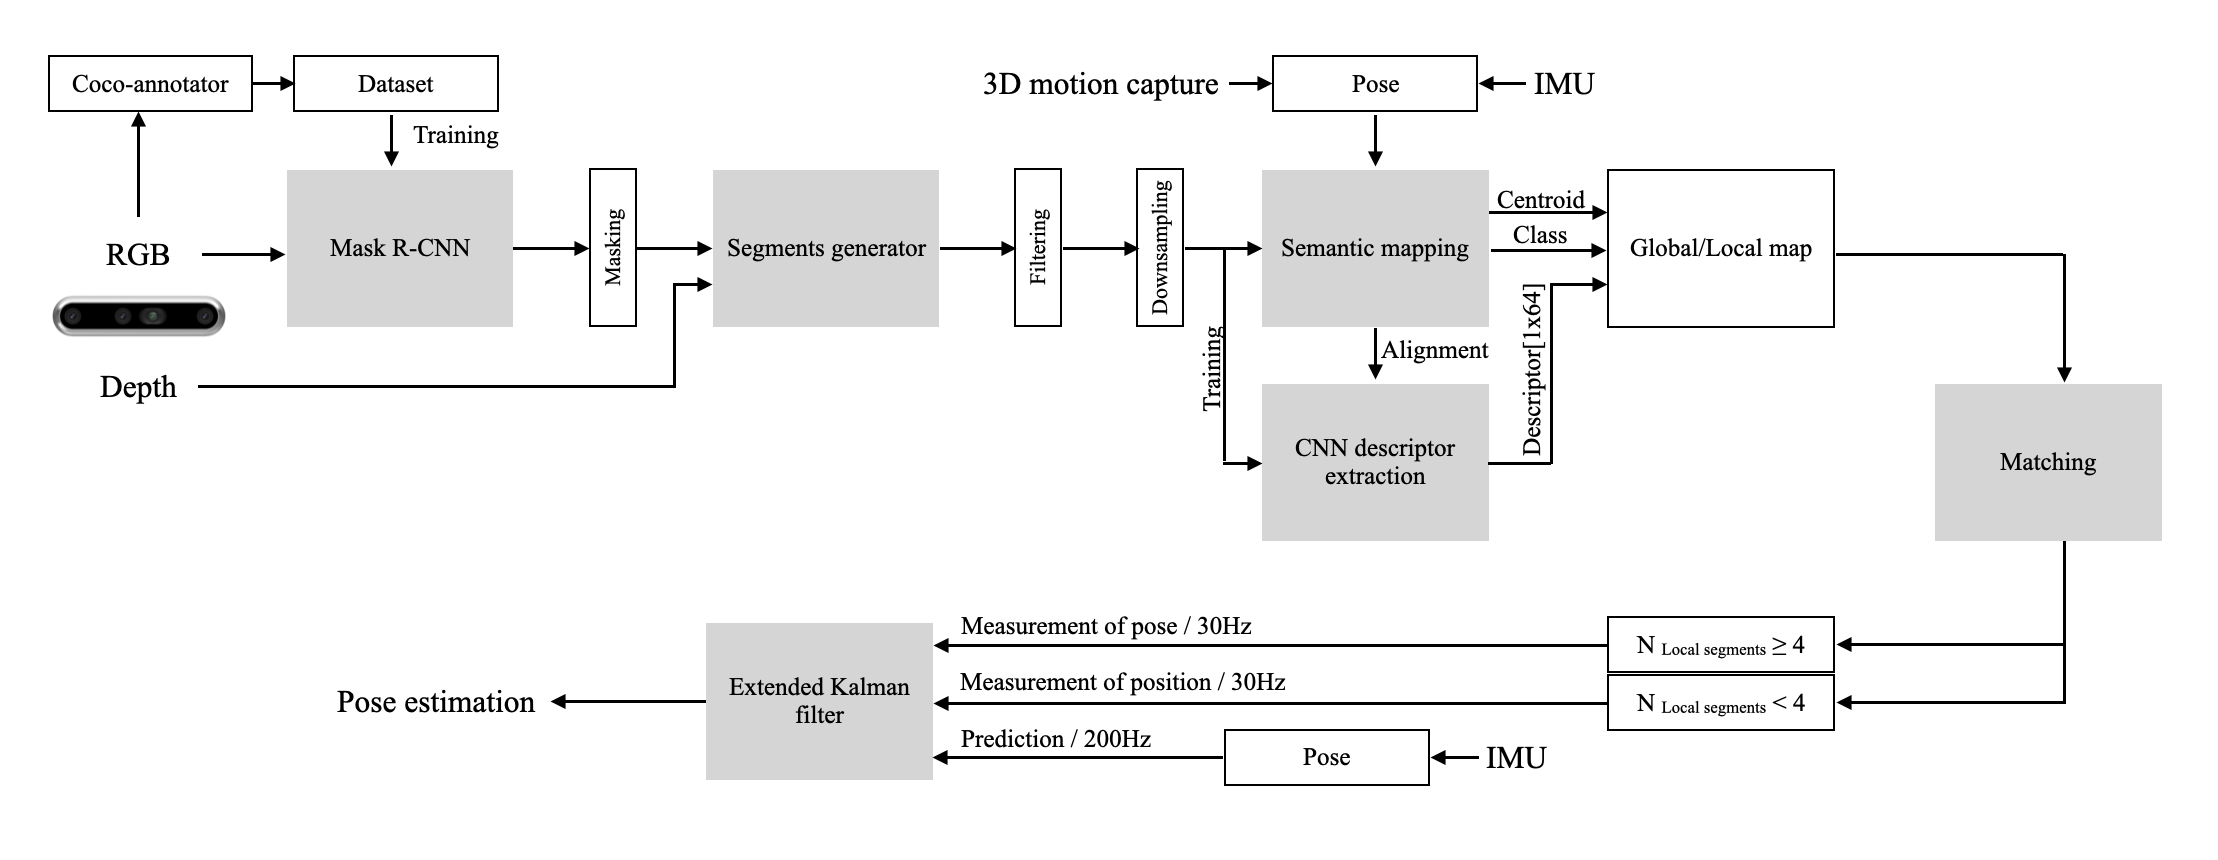
\includegraphics[width=1.0\textwidth]{Pictures/diagram_whole.png}
    \caption{\textbf{Segment-Based Mapping and Localization Pipeline Overview.} This pipeline starts with 2D segmentation using COCO Annotator\cite{cocoannotator} for training a Mask R-CNN model. Segments from point clouds, merged with depth and instance masks, are positioned using motion capture or IMU data. These segments train a \acrshort{cnn} to produce segment descriptors, which then are used to build global and local maps. Matching between maps at 30Hz aids in pose estimation, supplementing the main pose prediction from IMU data at 200Hz in an \acrshort{ekf}. The process enables real-time pose estimation and trajectory plotting.} 
    \label{fig:big_pic}
\end{figure}

\begin{figure}[H]
    \centering
    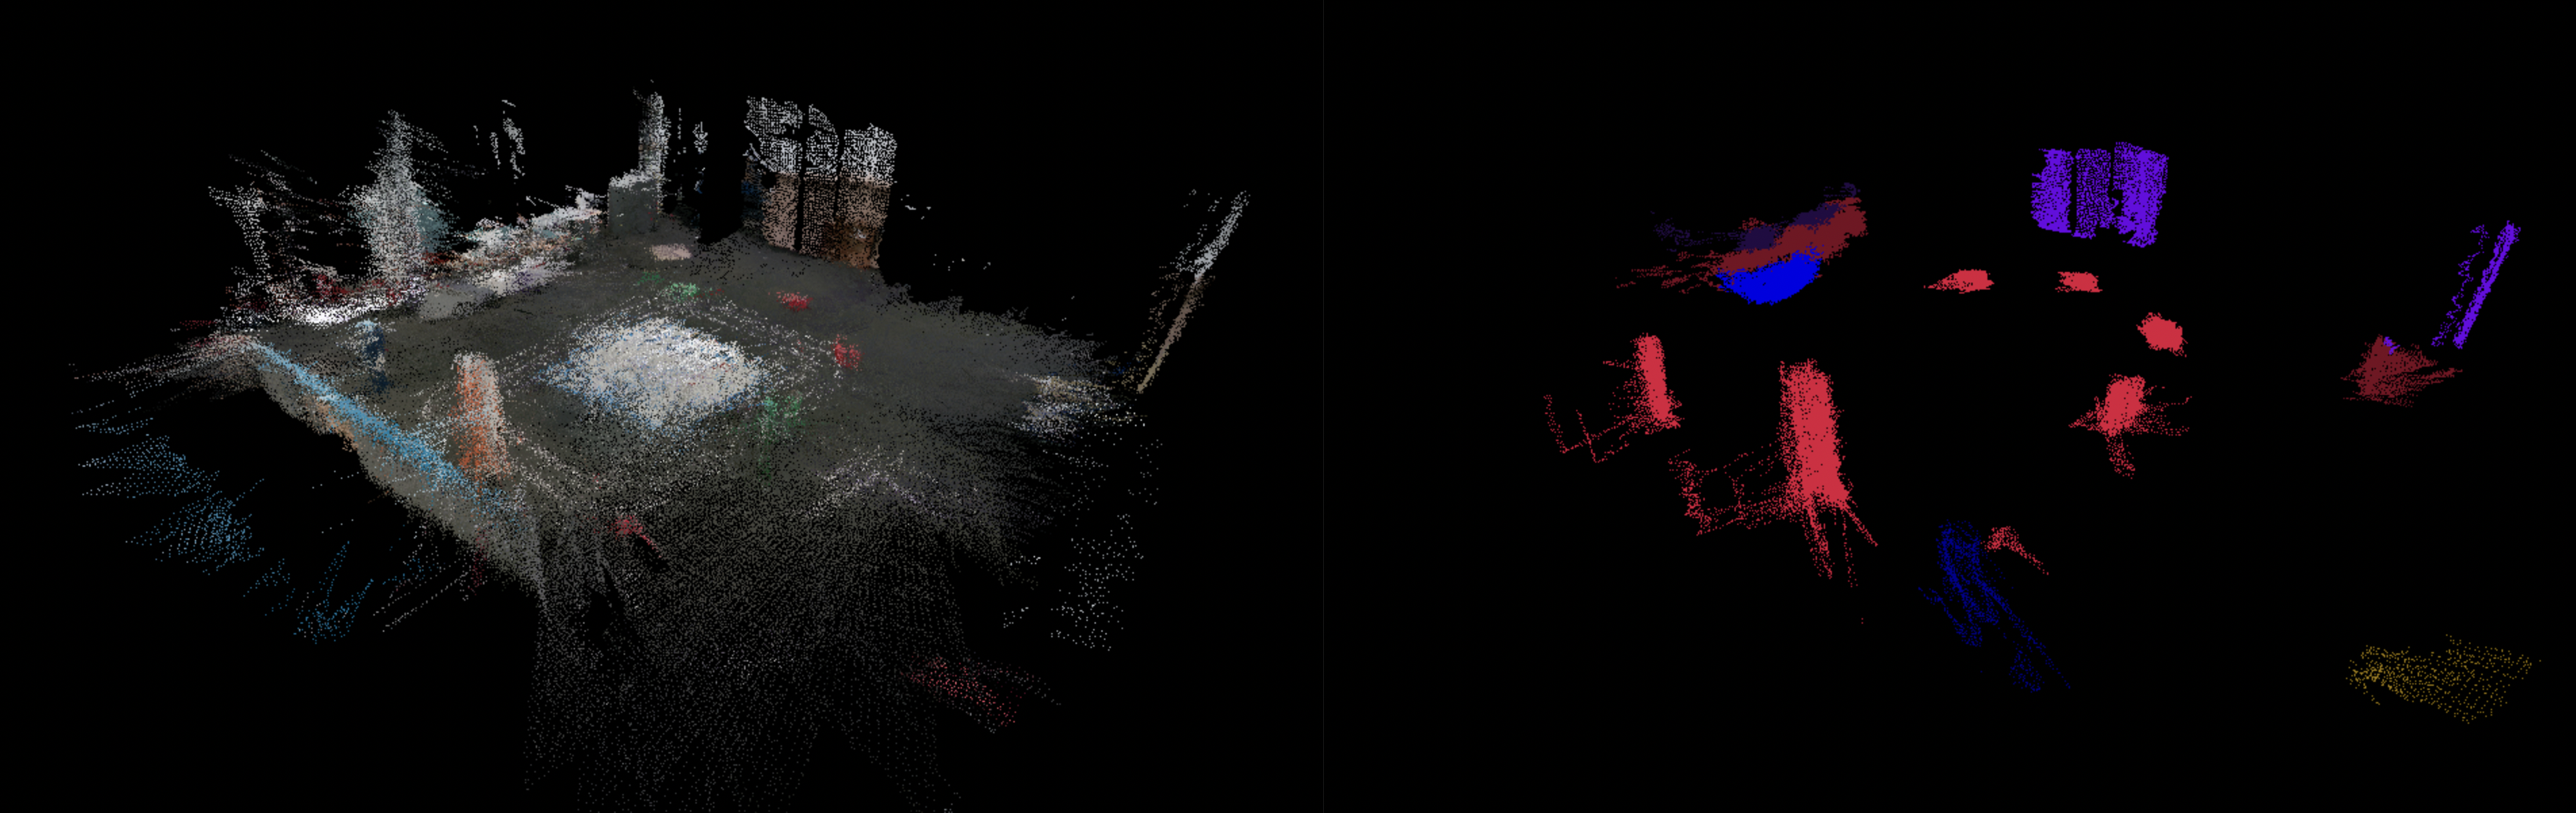
\includegraphics[width=1.0\textwidth]{Pictures/global_map_show.png}
    \caption{\textbf{Semantic Mapping from RGB-D Data.} This figure presents a semantic map covering an area of 10m x 10m, derived from data collected in \acrfull{asta} at \acrfull{dtu}, a large indoor infrastructure. The left image is created from the original RGB-D point cloud data, combined with global positioning obtained from the motion capture system in \acrshort{asta}. The right image is the result of augmenting semantic segments extracted using the methodology outlined in Fig.\ref{fig:seg_vis}. Additionally, noise reduction techniques have been applied to enhance the clarity and accuracy of the semantic map.}
    \label{fig:global map}
\end{figure}
\section{Environment of Data Caption}

Datasets are crucial for training and testing deep learning models, significantly impacting the performance of \acrshort{uavs} navigation systems. This thesis focuses on the importance of image datasets for training 2D instance segmentation models and the role of segments or point clouds for training 3D \acrshort{cnn} descriptor extraction models. These are vital for achieving accurate matching in a pre-existing map. Additionally, \acrshort{imu} data and accurate position ground truth are essential for evaluating the model's performance in localization tasks, especially when \acrshort{gnss} signals are unavailable and IMU data might introduce trajectory shift errors.

A notable challenge is that most existing 3D datasets are associated with LiDAR sensors, which have characteristics differing from 3D point clouds generated by RGB-D sensors. This disparity can affect final testing outcomes. Furthermore, most RGB-D datasets are based on indoor scenarios, which are not directly applicable to UAVs that require testing in medium or large-scale outdoor environments.

Given these challenges, creating a customized dataset for this thesis is both necessary and beneficial. Before data collection, it is essential to define the categories of objects to be included. Utilizing the resources available at \acrshort{asta} test facility, seven categories have been identified: Box, Building, Computer, Table, Chair, People, and Other. The 'People' category is specifically designed to detect dynamic elements, which are not considered valid instances for localization and are filtered out during segment generation. The instances from these categories are distributed over an area measuring 10m x 10m, as illustrated in Fig. \ref{fig:setting of enviroment}.
\begin{figure}[H]
    \centering
    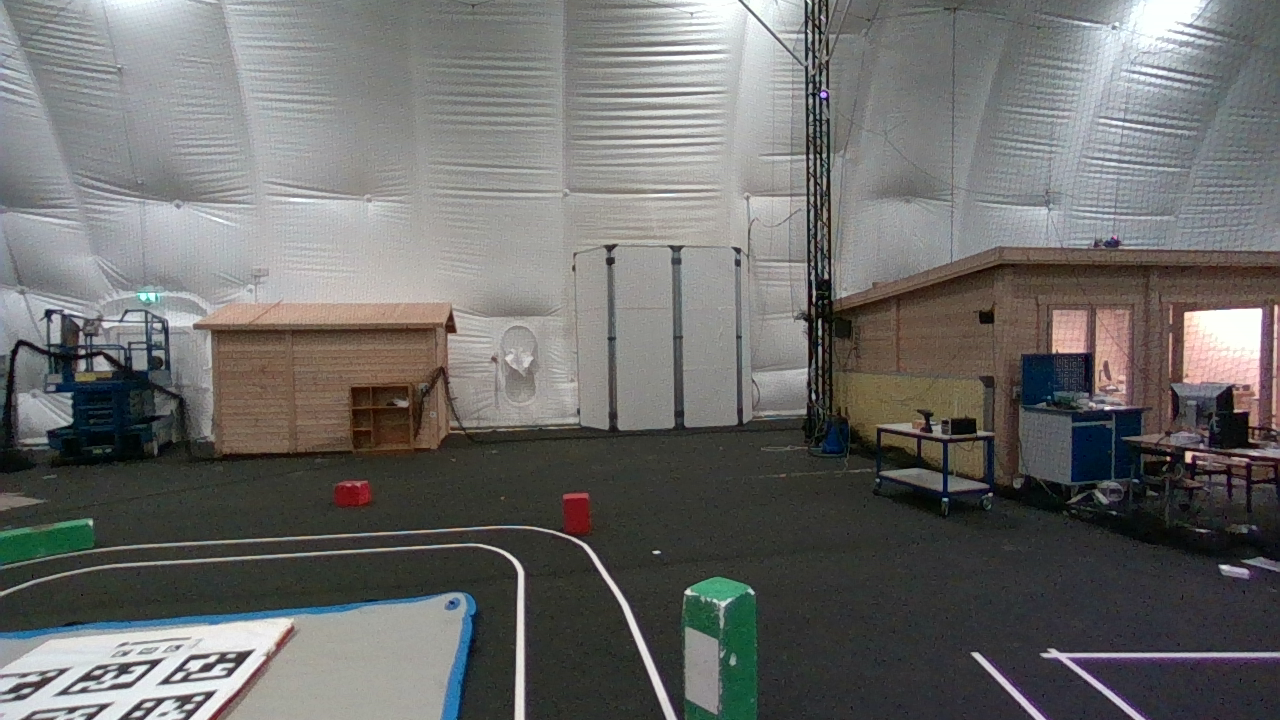
\includegraphics[width=.5\textwidth]{Pictures/rgb_1701886036.74969.png}\hfill
    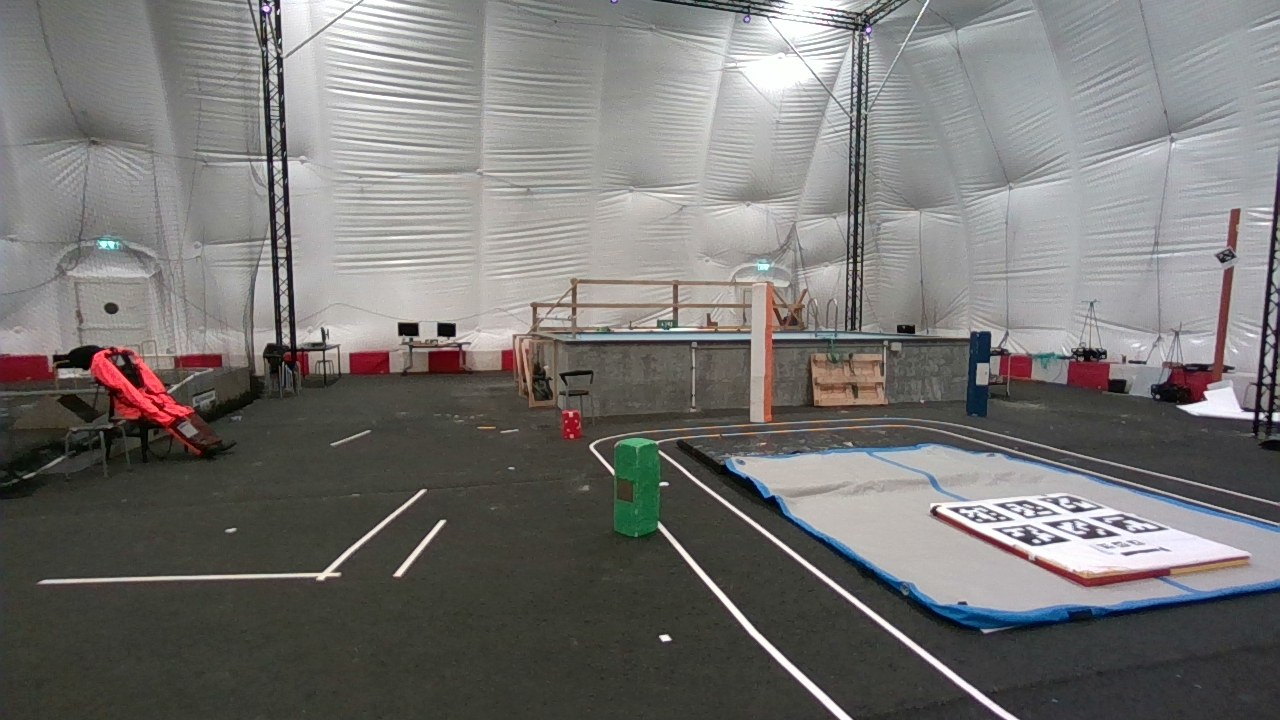
\includegraphics[width=.5\textwidth]{Pictures/rgb_1701886141.9452503.png}\hfill
    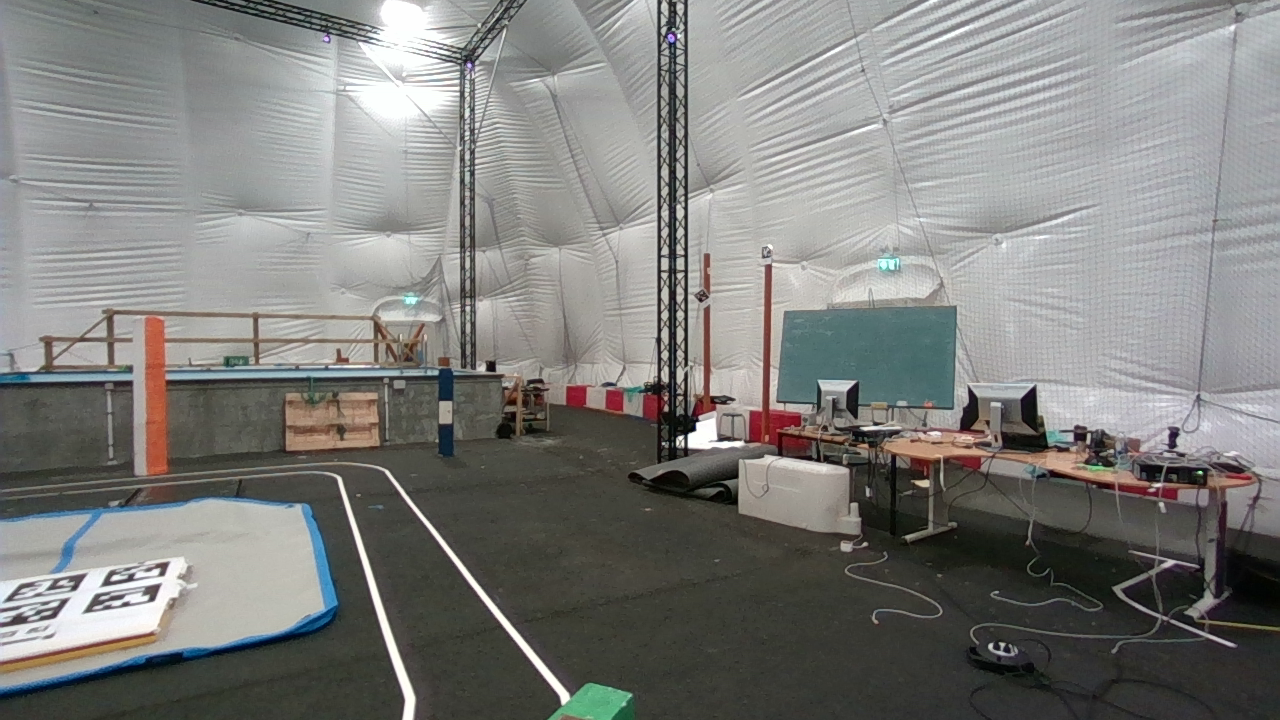
\includegraphics[width=.5\textwidth]{Pictures/rgb_1701886166.3457768.png}\hfill
    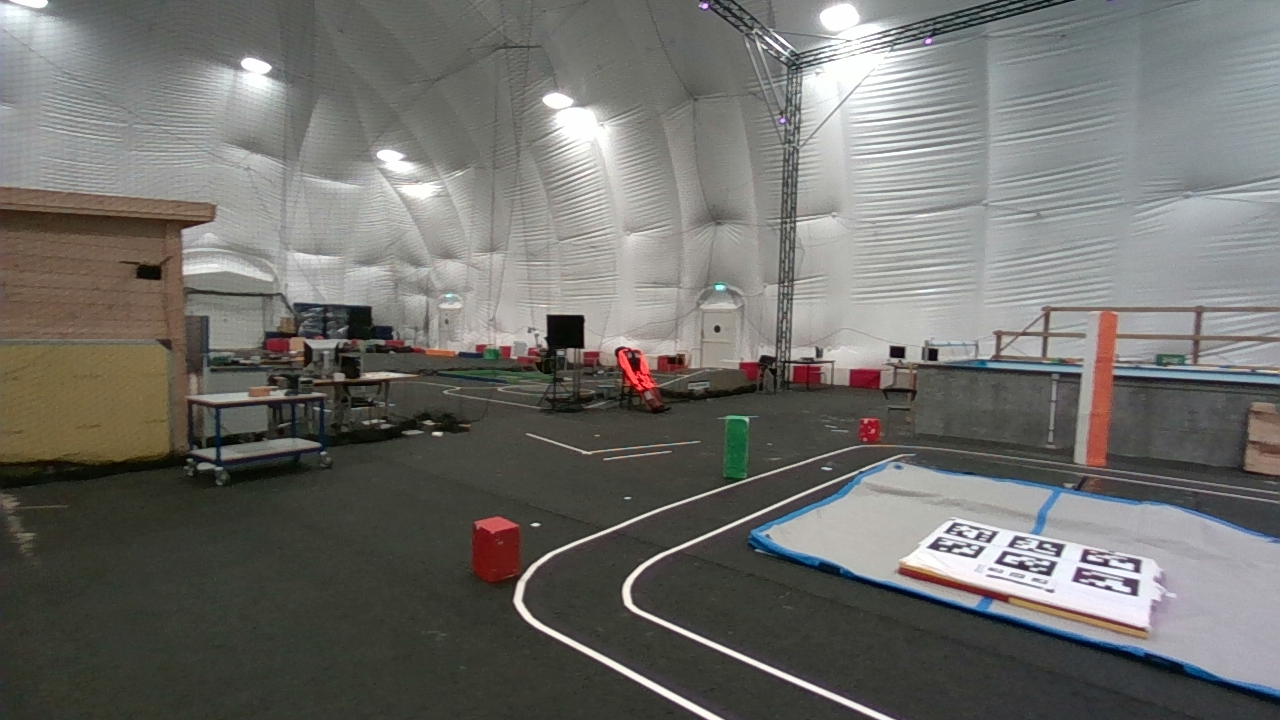
\includegraphics[width=.5\textwidth]{Pictures/rgb_1701886179.3437464.png}
    \caption{Setting of the Environment.}
    \label{fig:setting of enviroment}
\end{figure}

\section{Methods and Tools Used for Data Capture}

For data collection, the drone Holybro X500 V2, equipped with the Holybro Pixhawk 4 Autopilot Flight Controller, LattePanda 3 Delta, and Intel RealSense Depth Camera D455, is utilized.
\newline
\subsection{Ground Truth}
The 3D motion capture system at \acrshort{asta}, covering a 16m x 12m area with a camera height of 8m, provides the drone's pose in the world frame (Fig. \ref{fig:optitrack}). This system, featuring 16 Prime 17W cameras, boasts an accuracy of <5mm and repeatability of <1mm. To enable system detection of the drone, five reflective markers are attached, avoiding symmetrical placements. The drone, adorned with markers (Fig. \ref{fig:rfball}), is maneuvered in the space, allowing marker detection and selection as a rigid body in the Motive software. The data streaming pipeline from the motion capture system is pre-configured. Users must connect to the 'asta\_optitrack\_5G' local network and run the ROS client to initiate data streaming.

To remotely operate the Ubuntu 20.04 system running on the microcomputer Lattepanda aboard the drone, an OpenSSH server is employed. ROS Noetic is used to launch the ROS client in the VRPN workspace. The 'rosbag' command records topics containing information about the drone's pose and timestamps in the world frame at a rate of 100Hz. For clarity, this thesis will refer to this as the 'drone frame' to distinguish it from the IMU frame and RGB-D camera frame.


\subsection{Image Query}

RGB-D data is captured using the Python wrapper for the Intel RealSense camera, the 'pyrealsense2' package\cite{intelrealsense_librealsense_python}. Camera parameters are saved as a '.json' file. RGB and depth images are captured at a resolution of 640x480, with a frequency of 5Hz for training and mapping data, and 30Hz for real-world testing and evaluation. All imagery is stored on the microcomputer onboard the drone.
\newline
\subsection{IMU Data}

MAVLink is employed to establish communication between the drone and QGroundControl on the microcomputer. Flight logs, reflecting PX4 firmware 1.3 behavior, including IMU messages, are saved in '.ulg' files. For efficient data processing, these IMU data are converted into CSV files using the Python package 'pyulog'\cite{px4_pyulog}.

\section{Annotation and Split of Dataset}

\begin{figure}[H]
    \centering
    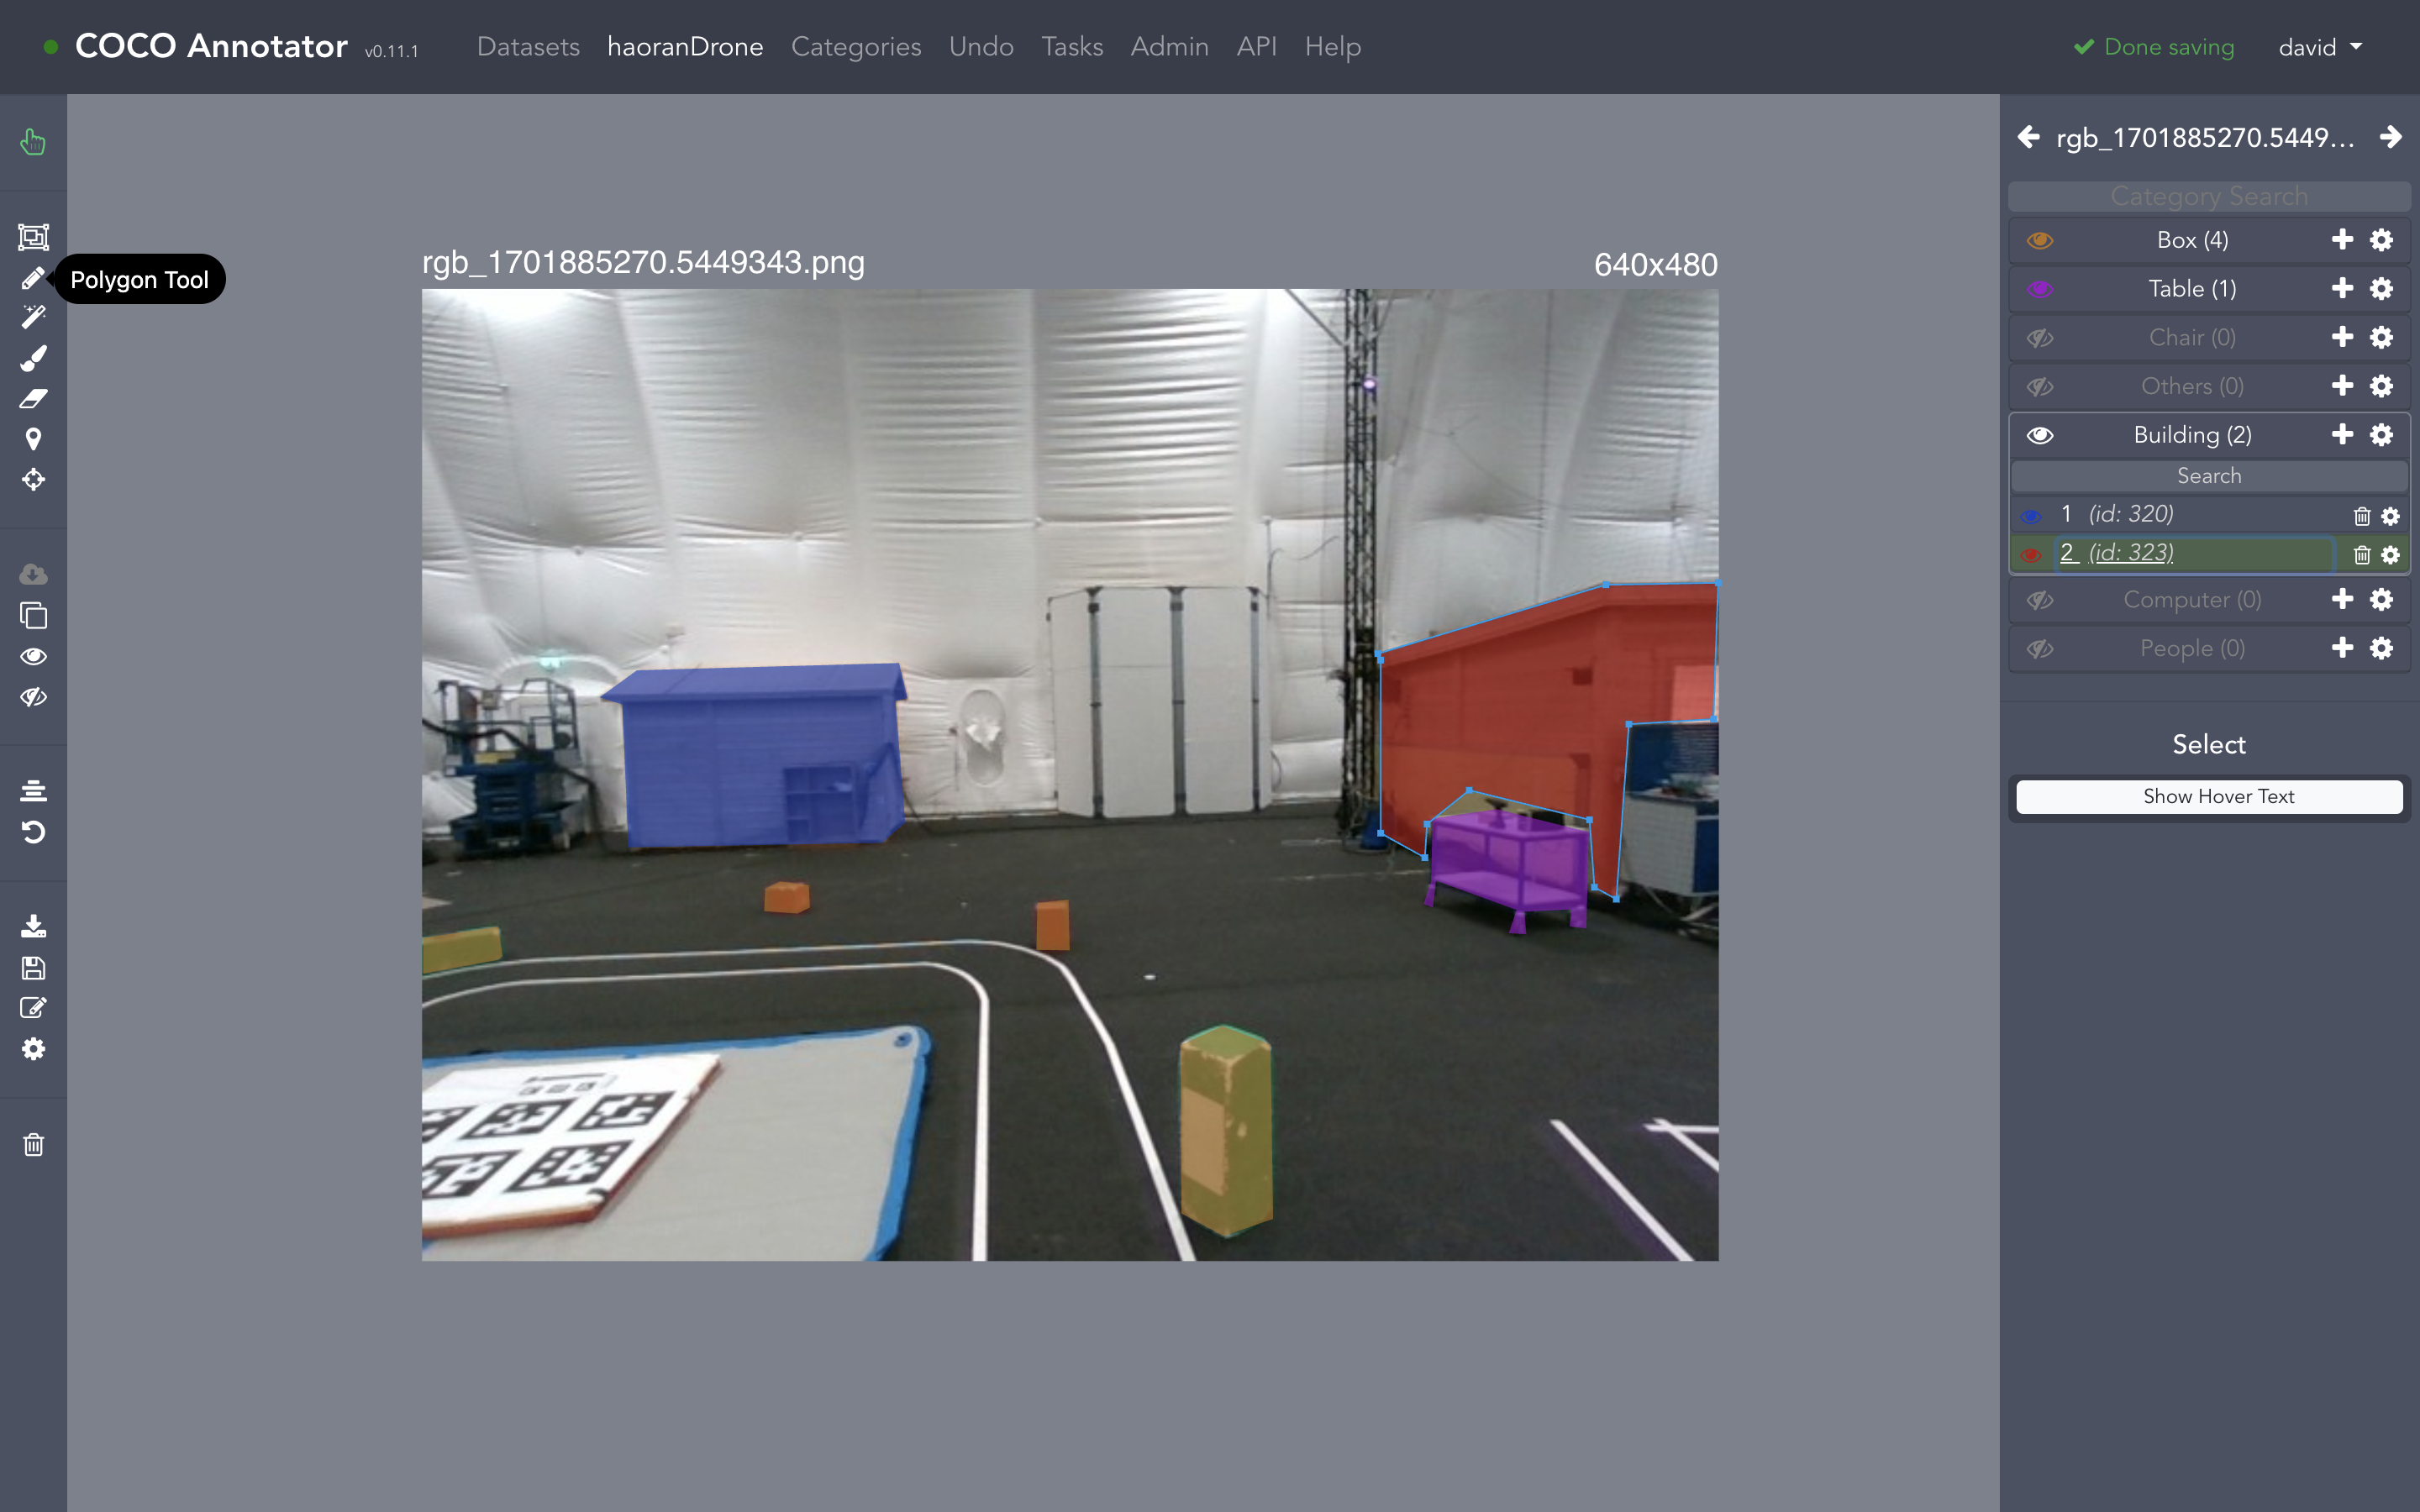
\includegraphics[width=.8\textwidth]{Pictures/cocoannotator/polygon.png}
    \caption{Illustration of Instance Segmentation Labeling.}
    \label{fig:polygon}
\end{figure}
\begin{figure}[H]
    \centering
    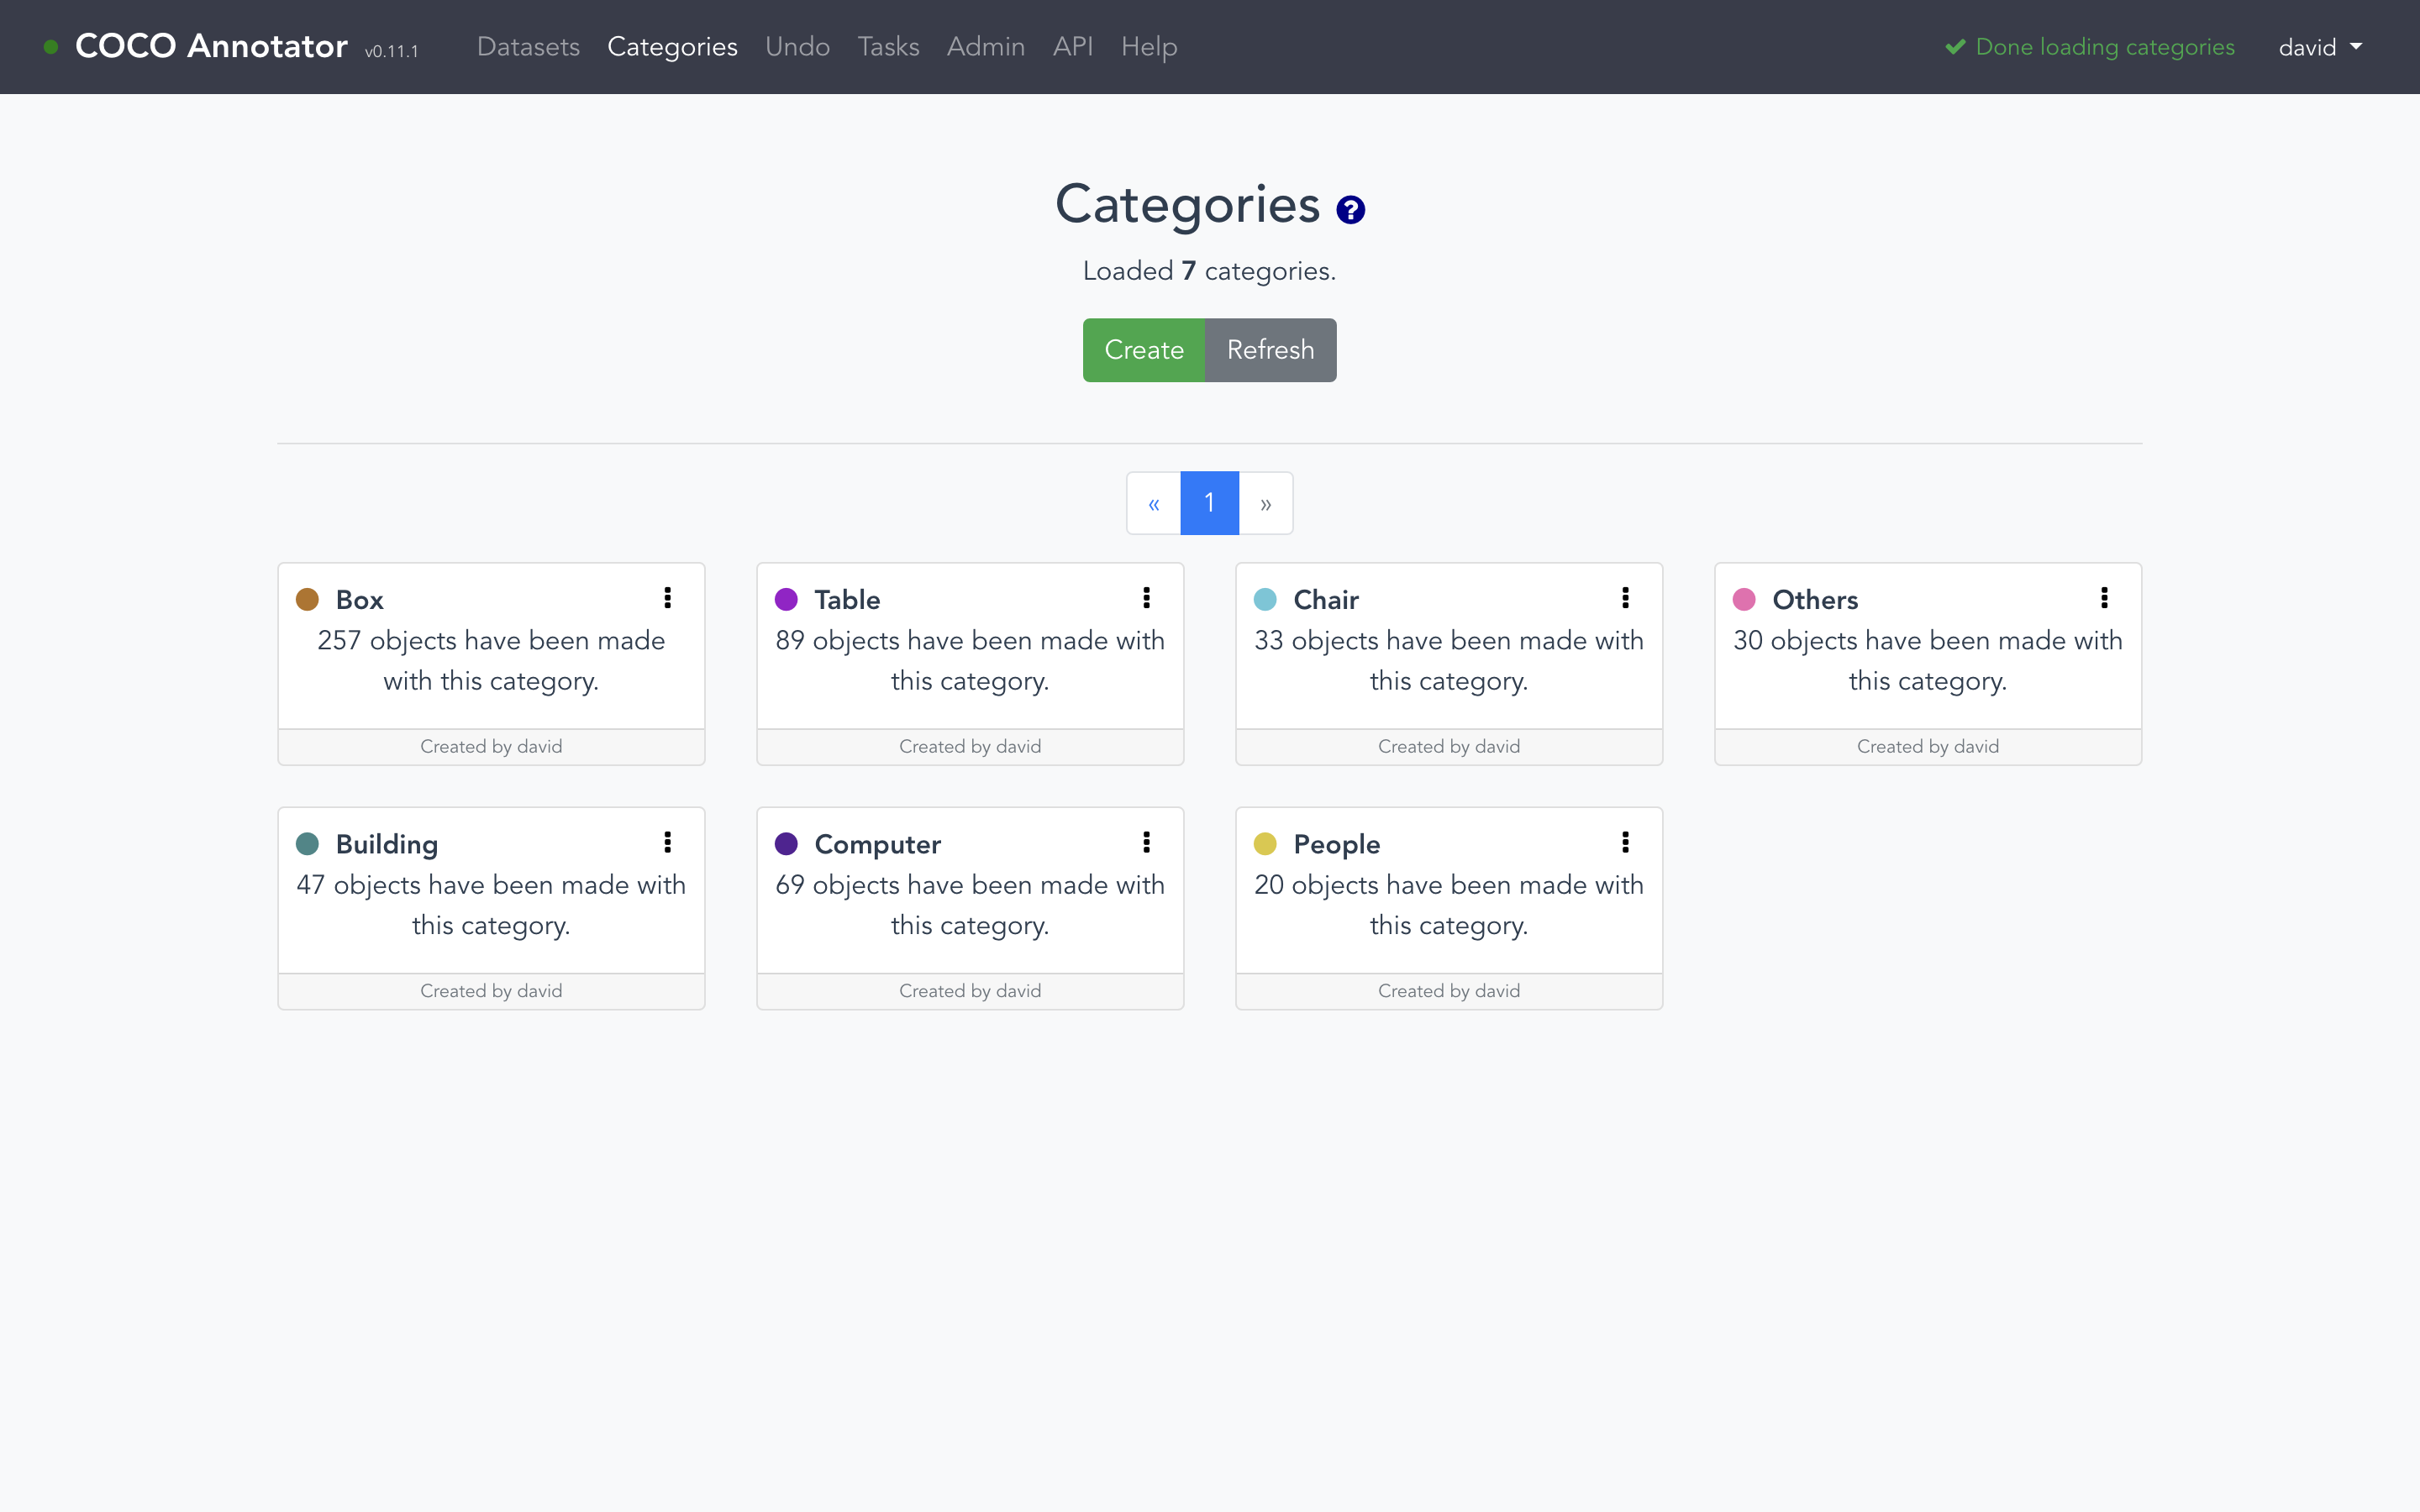
\includegraphics[width=.8\textwidth]{Pictures/cocoannotator/categories.png}
    \caption{Distribution of Categories in the Dataset.}
    \label{fig:datasetinfo}
\end{figure}

The preparation of a dataset is a key step in training a model to achieve optimal performance. For this project, a customized dataset comprising seven categories was developed. Initially, the dataset included raw images without segmentation labels. To facilitate customized annotation and meet training objectives, the COCO Annotator tool was employed for manual segmentation of raw RGB images in the COCO format. Figure \ref{fig:polygon} illustrates the process of creating polygons for segmentation. These polygons were drawn around objects falling within the seven predefined categories, allowing for the generation of annotations in the COCO format.

Subsequently, the dataset was enriched with these annotations, resulting in a total of 128 labeled images encompassing 545 labeled objects, as depicted in Figure \ref{fig:datasetinfo}. This annotated dataset forms the foundation for training the deep learning models for instance segmentation, ensuring that the models are tailored to the specific requirements of the project.

\section{2D Instance Segmentation}
This section introduces the 2D instance segmentation method, including model setup, GPU setup, and model evaluation.

\subsection{Mask R-CNN Settings}
The training configuration adopts a 1x schedule, a standard yet effective training strategy in mmdetection, which balances training time and model performance. The optimizer used is SGD (Stochastic Gradient Descent) with a learning rate of 0.02 and a weight decay of 0.0005, parameters chosen to optimize the learning process with small dataset. The model initializes with pre-trained weights from a Mask R-CNN model trained on the COCO dataset, which provides a solid foundation for learning the specific features of my custom dataset. It's notable that the structure of the pre-trained model is different from mine, but it still is meaningful to load only the same parts.

My dataset, annotated in the COCO format, includes a variety of classes like 'Box', 'Table', 'Chair', 'Others', 'Building', 'Computer', and 'People'. This diverse range of classes indicates a comprehensive approach to object detection and segmentation, allowing the model to learn and differentiate between all defined object types.

For the Region Proposal Network (RPN) and Region of Interest (ROI) heads, the default configuration have configured specific parameters such as anchor generation ratios and scales, bbox coding, and ROI extraction strategies. These settings are crucial for determining how the model proposes candidate object regions and how it processes these regions for accurate classification and segmentation.

The model employs predefined loss functions for bounding box prediction (L1Loss) and mask prediction (CrossEntropyLoss), ensuring precise segmentation of objects. Additionally, the classifier is configured to differentiate among 7 distinct classes, aligning with the diverse nature of the dataset.

Data augmentation and preprocessing are integral parts of the training pipeline. The model employs strategies like random resizing and flipping, enhancing the robustness of the model by exposing it to varied representations of input data.

For evaluation, the model's performance is assessed using standard COCO metrics for both bounding box accuracy and segmentation quality. This approach ensures a comprehensive evaluation of the model's effectiveness in both detecting objects and accurately segmenting them.

Regarding the settings for the training environment, such as CUDA settings for GPU acceleration and distributed training configurations, are essential for efficient training, especially when dealing with complex datasets. The model also incorporates visualization and logging mechanisms, facilitating effective monitoring and debugging during the training process. All outputs and intermediate results are organized and stored in a specified working directory, ensuring a structured approach to model development and evaluation.
\subsection{High Performance Computing (HPC) Settings}

For the instance segmentation task, This thesis utilized the HPC environment to train a Mask R-CNN model. A script was written to submit a job to the HPC facilities at DTU, using the LSF Resource Manager/Scheduler for job management. This script specifies various parameters for job execution, including queue type, job name, number of cores, GPU usage, memory requirements, and walltime limit.

In DTU's HPC environment, job scripts are essential for running applications in batch mode, minimizing human intervention. The script begins with the standard shebang line \texttt{\#!/bin/sh}, followed by \texttt{\#BSUB} commands as instructions to the LSF system. For example, \texttt{-q gpuv100} defines the queue type, \texttt{-J seg\_torchrun\_new\_config} sets the job name, and \texttt{-n 4} requests four cores.

A single GPU is allocated exclusively with \texttt{-gpu "num=1:mode=exclusive\_process"}. Memory requirements are specified as \texttt{-R "rusage[mem=3GB]"}, allocating 3GB of memory per core. The job's maximum duration is set with \texttt{-W 24:00}, limiting it to 24 hours.

The script then sets up the environment and executes commands. The line \texttt{conda activate forpred} activates a Python environment with necessary dependencies. Finally, \texttt{torchrun} initiates the Mask R-CNN model training.

\subsection{HPC Running Summary}
After completing the HPC job script, the resource usage report was sent by email. It shows the CPU usage was 52244.18 seconds, indicating that the 24-hour time wall was not exceeded. Maximum memory usage peaked at 7599 MB and averaged 6132.80 MB, while total memory requests were 12288.00 MB, suggesting that the task was within the memory allocation.

\subsection{Model Evaluation}

Model was evaluated by introducing mask loss, accuracy, and learning rate in this section.

\begin{figure}[H]
    \centering
    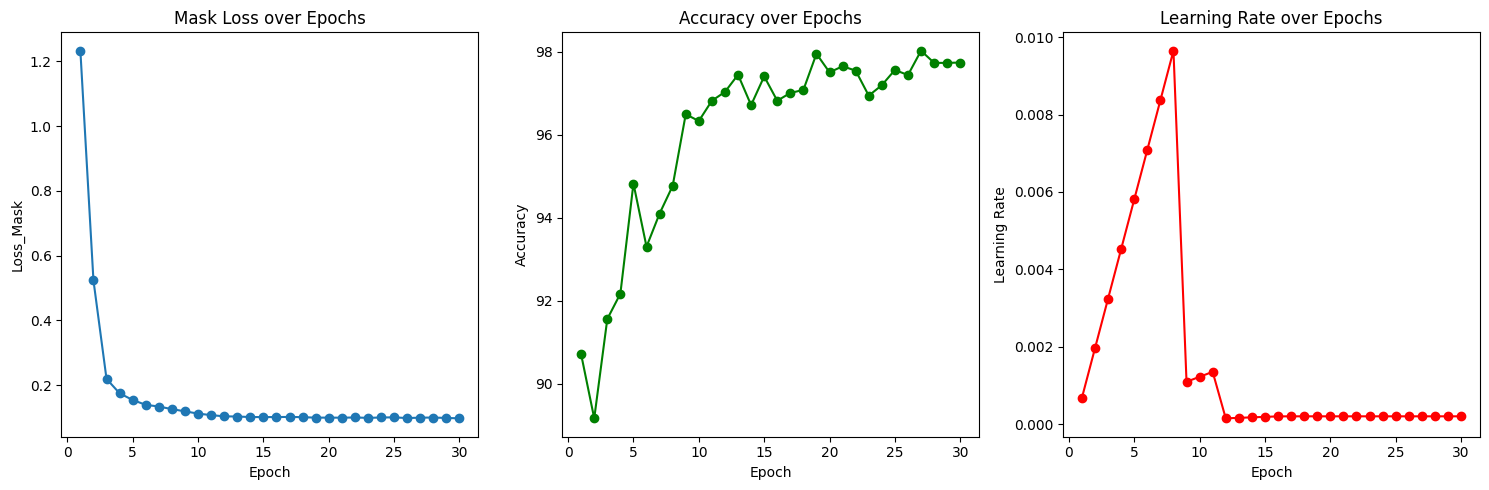
\includegraphics[width=.9\textwidth]{Pictures/maskrcnn/mask_loss_30.png}
    \caption{Mask Loss, Accuracy and Learning Rate over Epochs.}
    \label{fig:acc_train}
\end{figure}

From the Fig. \ref{fig:acc_train}, it's evident that the mask loss decreases over epochs, which suggests that the model is learning and improving its ability to segment the objects accurately.

The accuracy plot shows fluctuations, which is common in training as the model learns from different batches of data. However, the overall trend should ideally be upwards. The sharp dip seen around epoch 6 could be due to several reasons such as a bad batch of data, a need for regularization, or it could just be a random fluctuation.

A learning rate schedule where the learning rate increases initially and then decreases is a strategy to help the model converge faster while allowing fine adjustments as it gets closer to the minimum.

\begin{figure}[H]
    \centering
    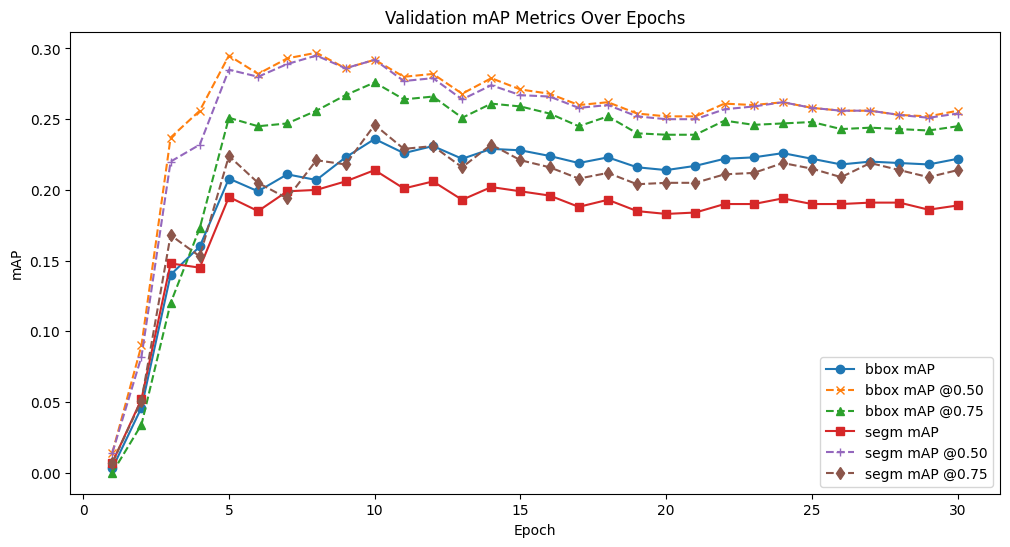
\includegraphics[width=.9\textwidth]{Pictures/maskrcnn/mAP_30.png}
    \caption{BBox and segm mAP over Epochs.}
    \label{fig:mAP}
\end{figure}
Fig.\ref{fig:mAP} shows the model's performance in terms of mAP metrics across validation epochs. The analysis of this plot reveals several insights:

\textbf{General Trend:} There is an upward trend in both bounding box (bbox) and segmentation (segm) mAP values across epochs, suggesting that the model is learning and improving its predictive accuracy over time.

\textbf{Fluctuations:} Some fluctuations in mAP values are observed, which is normal in the training process. These could be due to the model learning new patterns, overfitting on certain data points, or adjustments in the learning rate. Despite these fluctuations, the general trend should be upward.

\textbf{IoU Thresholds:} The mAP values at IoU=0.50 are consistently higher than at IoU=0.75. This is expected as a lower IoU threshold is less stringent. The improvement in mAP at IoU=0.75 suggests that the model is becoming more precise in its predictions.

\textbf{Comparison Between bbox and segm mAP:} Both bbox and segm mAP are crucial for evaluating the model's performance. Typically, bbox mAP is higher than segm mAP as segmentation is a more complex task. If the segm mAP is close to the bbox mAP, it indicates effective segmentation capability.

\textbf{Late Epochs Performance:} Towards the later epochs, a plateau or a slight decrease in certain mAP metrics is observed. This could indicate overfitting or that the model is reaching its performance limit with the current architecture and hyperparameters.

\textbf{Segmentation Performance:} The segm mAP shows significant improvement, which is noteworthy given the complexity of segmentation tasks. Comparable performance in both bbox and segm mAP suggests proficiency in detection and segmentation.

\begin{figure}[H]
    \centering
    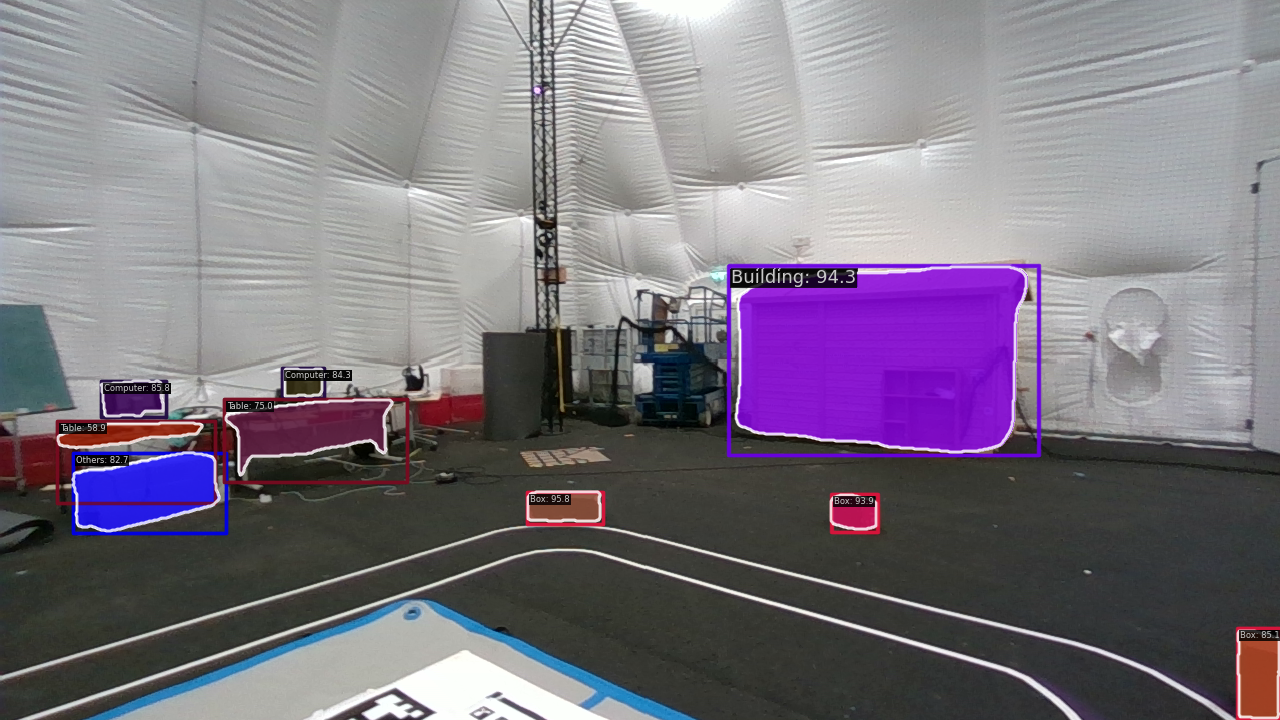
\includegraphics[width=.8\textwidth]{Pictures/maskrcnn/rgb_1701886047.947666.png}
    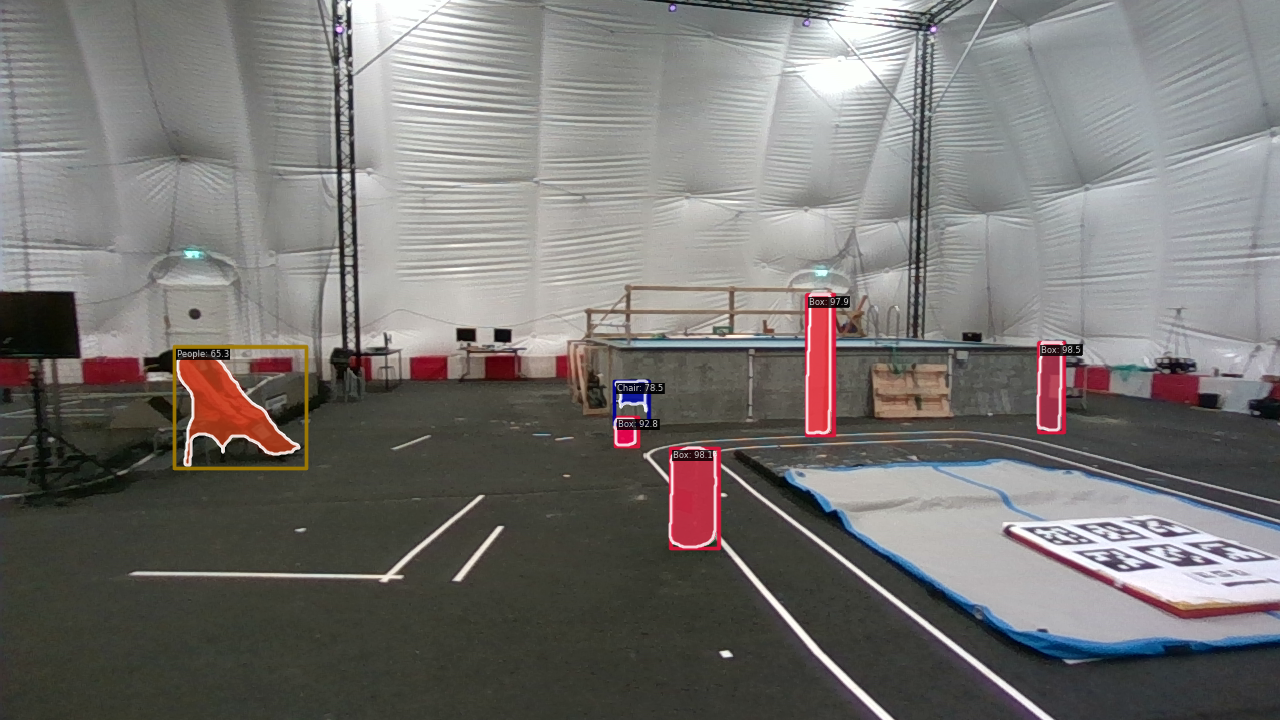
\includegraphics[width=.8\textwidth]{Pictures/maskrcnn/rgb_1701886140.9438705.png}
    \caption{Visualization of Mask R-CNN Instance Segmentation.}
    \label{fig:seg_pred}
\end{figure}

Figure \ref{fig:seg_pred} presents examples of the Mask R-CNN model's instance segmentation. The model effectively segments and classifies objects within a middle-scale environment. Detected instances are enclosed by bounding boxes, and segmentation masks accurately outline object contours. The model confidently classifies various objects, such as people and boxes, and closely adheres to object boundaries. This precision is crucial for applications requiring exact object localization and shape delineation. 

The provided visualizations show that the Mask R-CNN model is not only adept at detecting objects but also excels in accurately segmenting them, an essential aspect for practical applications in diverse environments. The high level of detail in the segmentation masks underscores the model's sophistication and its suitability for complex real-world applications.

\section{Segment Generator}

This section outlines the method used to generate segments in the form of colored point clouds. These segments are derived from instance segmentation and point clouds, which are in turn generated from corresponding depth images and camera parameters. Figure \ref{fig:seg_vis} visualizes this pipeline.

\begin{figure}[H]
    \centering  
    \includegraphics[width=1.0\textwidth]{Pictures/segments_extractor.png}
    \caption{\textbf{Visualization of Segments Extraction Process.} The procedure initiates with RGB-D data acquisition. A trained Mask R-CNN model then performs 2D instance segmentation. For each identified instance, a mask and label are generated, leading to the creation of distinct segments within the camera frame. These segments are subsequently color-coded based on a palette of seven unique labels.}
    \label{fig:seg_vis}
\end{figure}

Employing the best-performing Mask R-CNN model from the HPC, instance segmentation is executed on RGB images, with predictions such as masks, scores, and labels saved in a .json file. Notably, \acrfull{rle}, a form of lossless data compression, is utilized to encode masks for efficient storage. Pycocotools, part of the COCO API\cite{COCOAPI}, is then used to decode these masks from \acrshort{rle} format.

The framework designed for segment extraction leverages the rich data obtained from RGB image instance segmentation to generate colored segments for each identified instance. Figure \ref{fig:seg_pipeline} presents the algorithmic flow of this process.

\begin{figure}[H]
    \centering
    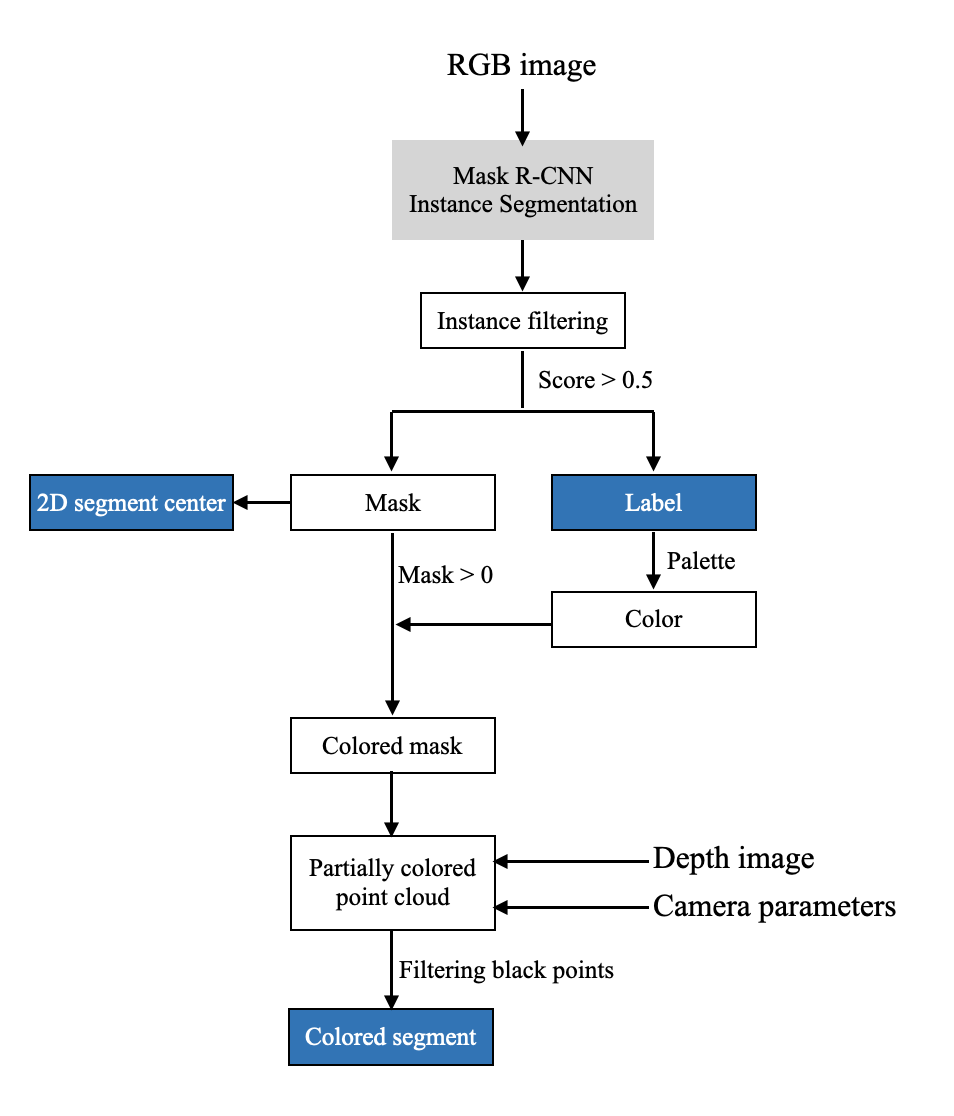
\includegraphics[width=.8\textwidth]{Pictures/Segment_extractor_diagram.png}
    \caption{Algorithmic Flow of Segment Extraction.}
    \label{fig:seg_pipeline}
\end{figure}

The process filters out instances with a confidence score below 0.5, ensuring only those with a high likelihood of accurate label prediction are retained. A dictionary maps each label to a specific color, which is then applied to pixels where the mask is positive. Additionally, the 2D segment center and label are recorded for later use. 

The next step involves combining the colored mask with the depth image and camera parameters, including depth camera intrinsics and scale, to generate a colored point cloud. Points that do not correspond to any segment (i.e., black points) are removed, leaving only the points with the designated color for each segment. This filtered point cloud represents the final output, serving as a colored segment for each individual instance.

This process not only ensures accurate segmentation but also adds a layer of interpretability by color-coding each segment according to its category. The innovative framework effectively utilizes the information from instance segmentation to enrich the point cloud data, providing a more comprehensive and visually intuitive understanding of the scene and the objects within it.

The segments generated through this method are integral for further analysis and applications where precise object localization and characterization are essential. By combining the depth information from the point clouds with the detailed segmentation from the Mask R-CNN model, this approach effectively bridges the gap between 2D image analysis and 3D spatial representation.

\section{Descriptor Extraction}

This module focuses on the extraction of descriptors from segments aligned in the world frame. Utilizing eigenvalues, the process generates descriptors of size [1x64] for matching in a pre-existing map after the training process. The CNN model employed for training is adapted from the SegMap codebase\cite{segmap,segmap2,segmatch2017}, which is documented in the segmappy branch\cite{segmmappy}.

\subsection{Model Setting}

\textbf{SegMap's CNN Model} The original CNN model from the SegMap project was based on TensorFlow 1.x, which necessitated explicit session management and a more complex coding style. Adapting to TensorFlow 2.x entailed significant modifications to simplify the code and ensure compatibility. 

The model begins with an input layer tailored for 3D data, followed by several convolutional layers with ReLU activation for feature extraction. Interspersed with these are max pooling layers, which reduce data dimensionality and enhance feature detection efficiency. Batch normalization and dropout techniques are incorporated to promote training stability and mitigate overfitting. Following a flattening step, the model integrates additional scales data into dense layers for more profound feature analysis. Furthermore, the model incorporates a reconstruction network with deconvolutional layers, characteristic of autoencoder structures. The architecture's optimization uses softmax cross-entropy for classification and reconstruction loss, with the Adam optimizer overseeing the learning process. 

\subsection{Prepocessing of Dataset}
\textbf{Filtering and Downsampling}
Given segments from segment generator and transformed from camera frame to world frame, Open3D, a versatile library used for 3D data processing is used to filter out point cloud segments with number of points fewer than a threshold and then apply a downsampling method to ensure the number of points in each segment falls within a desired range.

In the approach using Open3D, point cloud segments are first evaluated to ensure they contain a sufficient number of points, specifically more than 900. This step is crucial for maintaining a level of detail adequate for further processing. Segments that don't meet this threshold are excluded from the analysis. 

For those segments that do qualify, a voxel-based downsampling method is applied. This technique consolidates points within cubic voxels of a predetermined size (0.05 in this case), effectively reducing the point cloud's density. This downsampling not only enhances computational efficiency by decreasing the number of points but also helps in mitigating noise, thereby refining the quality of the data. 

While the goal is to retain point counts in the range of 100 to 5000, this specific range control isn't directly addressed in the snippet. However, it can be managed by adjusting the voxel size parameter, which influences the resultant point density post-downsampling. Such adjustments ensure that the final point cloud segments are neither too sparse nor excessively dense, making them suitable for accurate and efficient 3D analysis.

\textbf{Saving of All segments, positions, timestamps, labels and 2D centers} A structured approach is designed to save various types of information related to point cloud segments into CSV files. This is achieved through the \texttt{save\_all\_info} function, which orchestrates the recording of point cloud data, timestamps, segments' center positions in world frame, labels, and 2D centers, each into separate CSV files.

Within \texttt{save\_all\_info}, specific sub-functions are dedicated to handling distinct data types. The \texttt{write\_to\_segments} function stores the spatial coordinates of each point in the point cloud along with associated image and segment identifiers. Timestamps are logged through the \texttt{write\_to\_timestamps} function, linking each time point to the corresponding image and segment. The \texttt{write\_to\_positions} function captures the 3D center positions of segments in the world frame. Additionally, segment labels are stored using the \texttt{write\_to\_labels} function, facilitating future matching algorithms. These segments' center positions are crucial as they provide the real-world spatial context of the point cloud data.

Additionally, the code includes functionality to record the 2D centers of these segments in image coordinates. This data, representing the segments' locations in pixel coordinates, is critical for image-based analysis and calculations.

Storing both the 3D positions in the world frame and the 2D pixel coordinates in the image is a strategic step in preparing for the Perspective-n-Point (PnP) problem. The combination of these two types of data enables the accurate calculation of the drone's pose by correlating points in the image frame with their counterparts in the world frame, a key aspect of spatial orientation and navigation tasks in drone operations.

By ensuring that each piece of information – from spatial coordinates to temporal and categorical data – is meticulously recorded and organized, the \texttt{save\_all\_info} function sets the stage for advanced processing and analysis, including dataset preparation for CNN model and the crucial task of computing the drone's pose using PnP algorithms in the subsequent part of this thesis.


\subsection{HPC Settings}
This section elaborate on the utilization of \acrshort{hpc} for training a CNN model, following the earlier application for Mask R-CNN model training. 

\textit{Job Submission Script:}
My script, tailored for DTU's HPC facility, orchestrates a training job leveraging the LSF Resource Manager/Scheduler. It commences with a shebang \texttt{\#!/bin/sh} and employs \texttt{\#BSUB} directives to delineate job specifications. These include queue assignment \texttt{\#BSUB -q gpuv100} for GPU usage, job naming \texttt{\#BSUB -J train\_cnn}, core allocation \texttt{\#BSUB -n 4} for four cores, and exclusive GPU access. Memory requirements are explicitly stated, requesting 4GB per core and specifying host and GPU characteristics to optimize performance. A walltime limit of 18 hours is set, alongside notification and output file configurations.

The script's latter part focuses on the environment setup, activating a Conda environment and loading modules like CUDA, cuDNN, and TensorRT, essential for GPU-accelerated computation in neural networks. The execution of the training script 

\textit{Integration of CUDA for TensorFlow 2.x:} The HPC environment's configuration for TensorFlow 2.x involves specific CUDA settings. As per DTU HPC's guidelines\cite{dtu_hpc_cuda}, configuring TensorFlow to leverage CUDA enables efficient GPU usage, vital for accelerating deep learning computations. This setup ensures TensorFlow's compatibility with the available GPU resources, maximizing computational efficiency and significantly reducing training time for the CNN model.
\subsection{HPC Running Summary}
The job log reflects successful execution, indicating start and completion times. The resource summary reveals a CPU time usage of  20799.21 seconds and memory consumption peaking at 2847 MB, against a larger requested quota. The job's runtime and turnaround time fit well within the allocated limits.

\subsection{Model Evaluation}
CNN model was evaluated by reconstruction loss and training accuracy.
\begin{figure}[H]
    \centering
    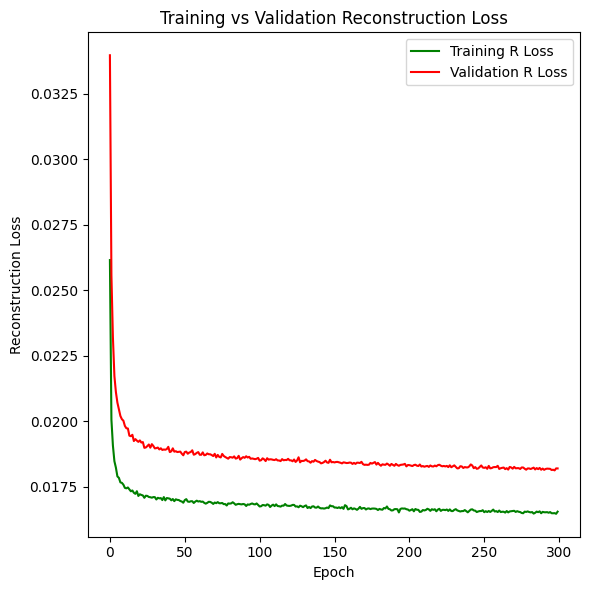
\includegraphics[width=.6\linewidth]{Pictures/R_loss.png}
    \caption{Training vs Validation Reconstruction Loss}
    \label{fig:cnn_plot}
\end{figure}

For a deep learning model to be robust and to mitigate the risk of overfitting, training it on a large and diverse dataset is crucial. In this thesis, the dataset for training is augmented with a substantial dataset derived from the KITTI odometry dataset\cite{Geiger2012CVPR}, which has been manually annotated by SegMap researchers\cite{segmap}. This approach ensures a rich and varied training environment for the model.

The effectiveness of the training process is evident from the significant decrease in reconstruction loss observed in both the training and validation phases, as shown in Figure \ref{fig:cnn_plot}. This reduction in loss indicates that the model is learning effectively from the data and improving its ability to reconstruct the input. Notably, the training accuracy achieved is approximately 50\%. While this might appear modest, it is significant in the context of the complex tasks the model is performing. This level of accuracy, in conjunction with the observed loss reduction, suggests that the model is training effectively and achieving a good balance between learning from the training data and generalizing to new, unseen data.

It's important to note that training accuracy alone is not the sole indicator of a model's effectiveness. The decrease in reconstruction loss is a strong indicator that the model is capturing the underlying patterns in the data, which is critical for tasks such as descriptor extraction and instance segmentation. These results suggest that the model is well-suited for these tasks and has the potential to perform effectively in practical applications.

\section{Global/Local Map Generator}
This section will explain the process of creating a comprehensive 3D map by transforming point cloud data from the camera frame to the world frame. This transformation is integral to the generation of both global and local maps, each with its unique methodology and data integration process.

\textbf{Global Map Generation:} The transformation from the drone to the world frame is precisely determined by the motion capture system. This high level of accuracy allows for the effective alignment of each segmented point cloud in camera frame with its corresponding pose in the world frame. 

These segments are initially identified in the camera frame, utilizing a 2D instance segmentation model. This model not only detects the segments but also provides critical data such as the 2D image pixel center and the associated label for each segment. Additionally, a high-dimensional descriptor generated from a \acrshort{cnn} model enriches the segment data, contributing to a more detailed and informative global map.

The following plots in Fig. \ref{fig:gt_2d} and Fig. \ref{fig:gt_3d} shows trajectories when capturing the data at ASTA. Notably, the second columns of both 3D and 2D show trajectories that used for generation of global map.

\begin{figure}[H]
    \centering
    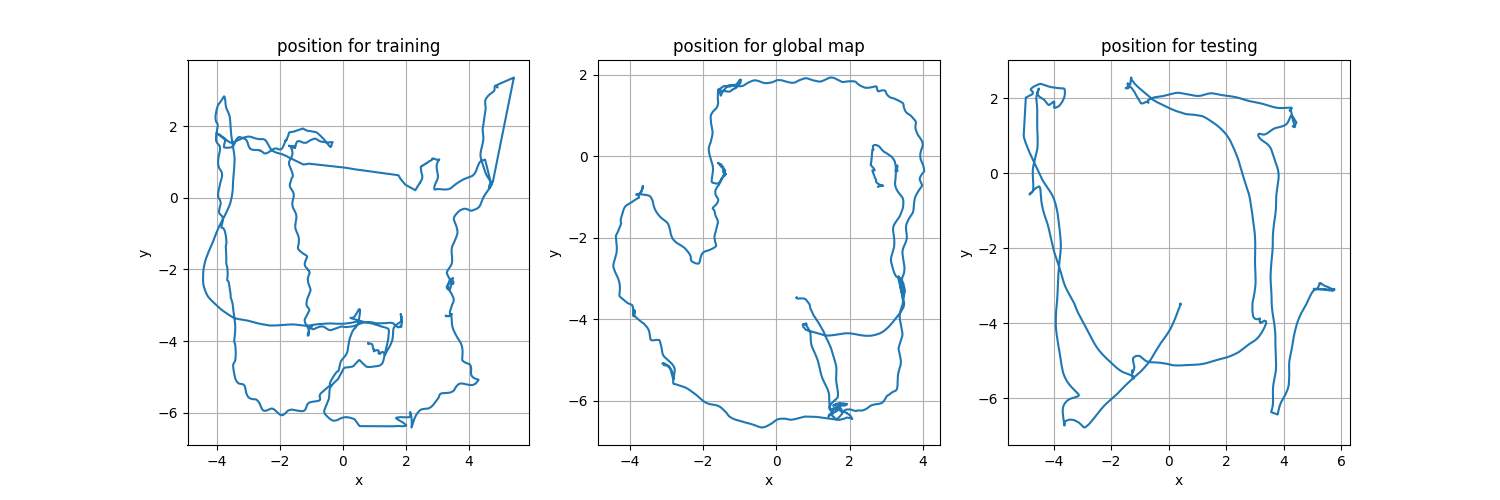
\includegraphics[width=1\linewidth]{Pictures/mapping/3gt.png}
    \caption{2D Trajectories of Data Capture}
    \label{fig:gt_2d}
\end{figure}

\begin{figure}[H]
    \centering
    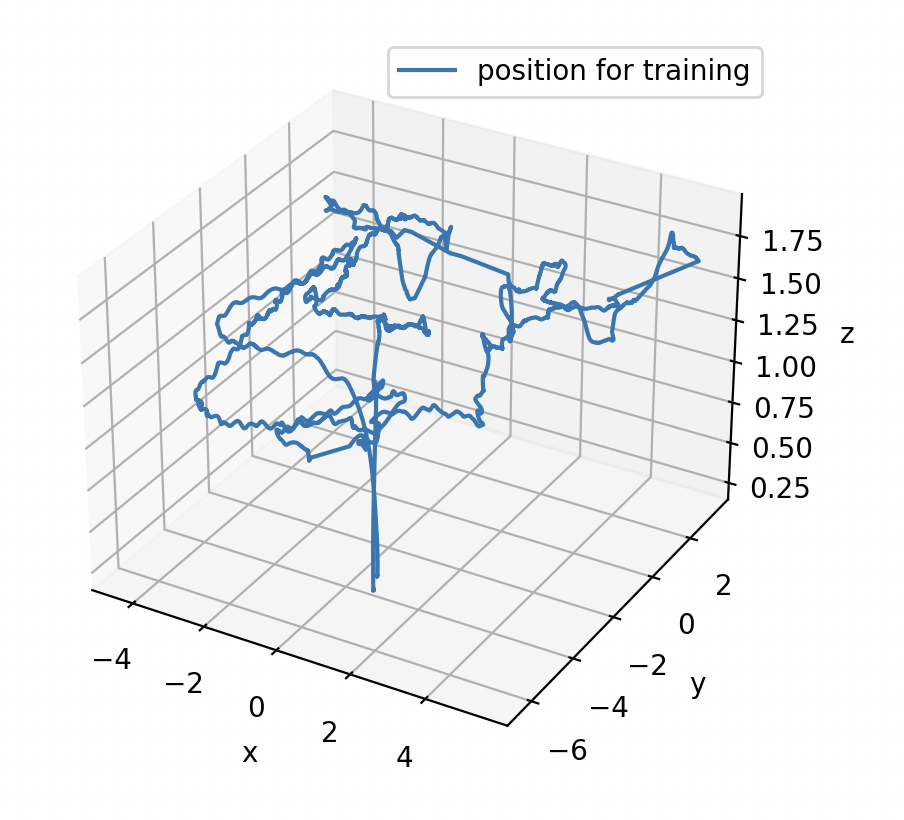
\includegraphics[width=.3\linewidth]{Pictures/mapping/gt_train.png}\hfill
    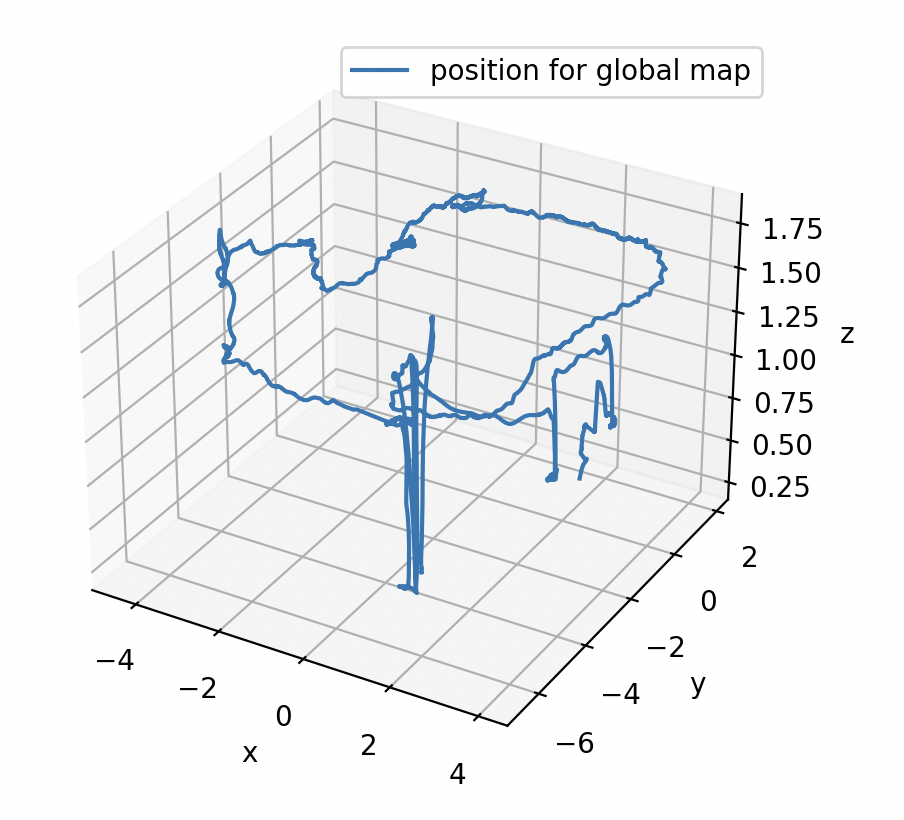
\includegraphics[width=.3\linewidth]{Pictures/mapping/gt_global.png}\hfill
    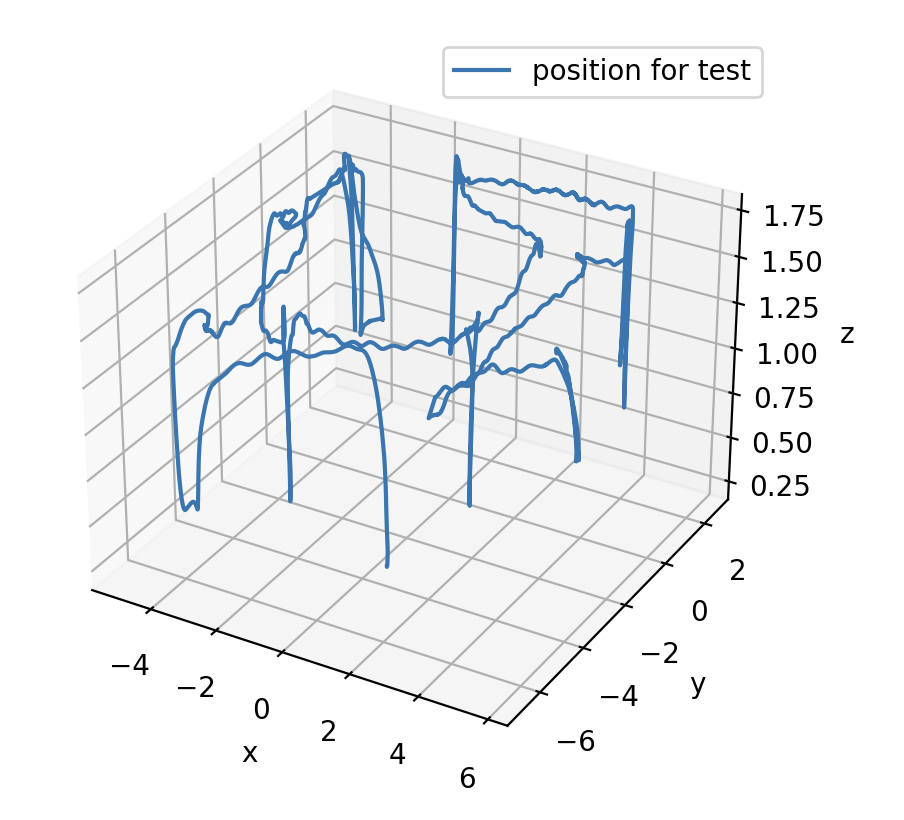
\includegraphics[width=.3\linewidth]{Pictures/mapping/gt_test.png}
    \caption{3D Trajectories of Data Capture}
    \label{fig:gt_3d}
\end{figure}


\begin{figure}[H]
    \centering
    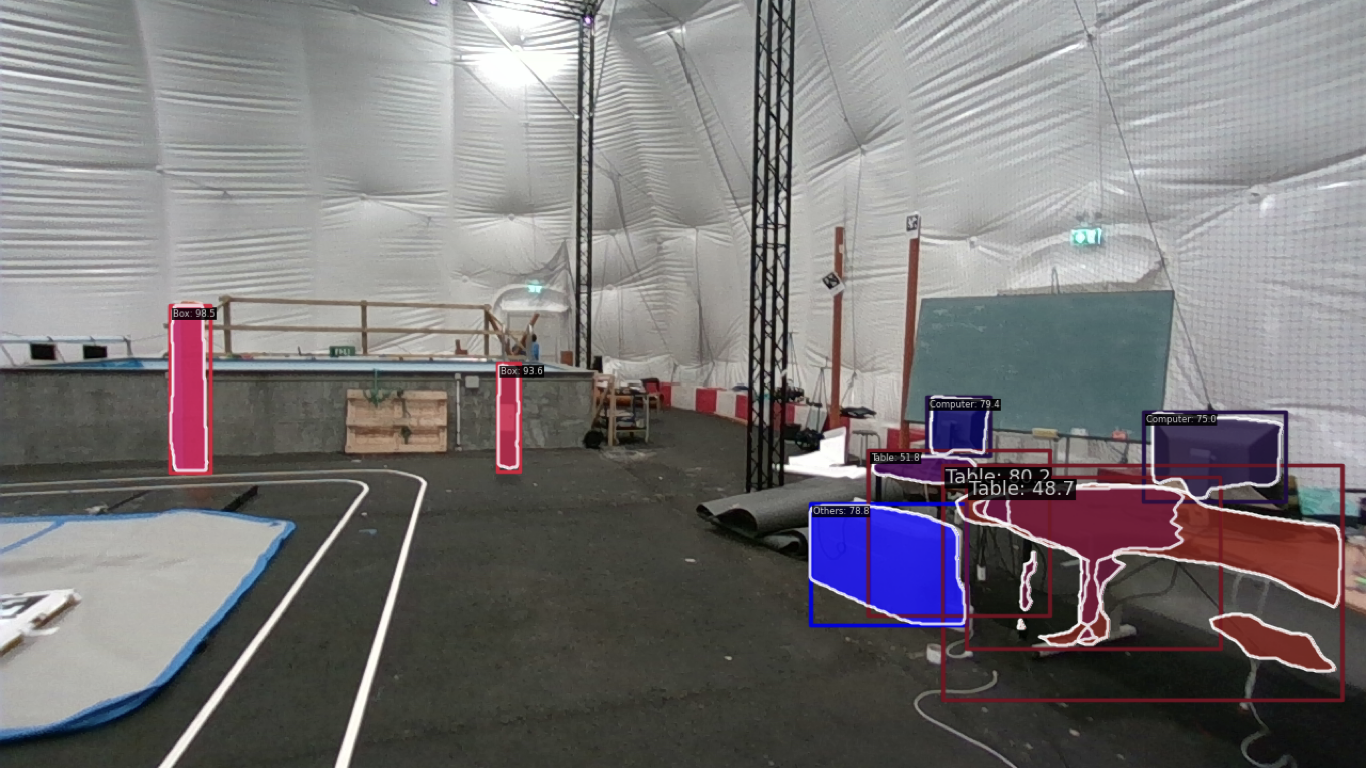
\includegraphics[width=.5\linewidth]{Pictures/mapping/vis_rgb.png}\hfill
    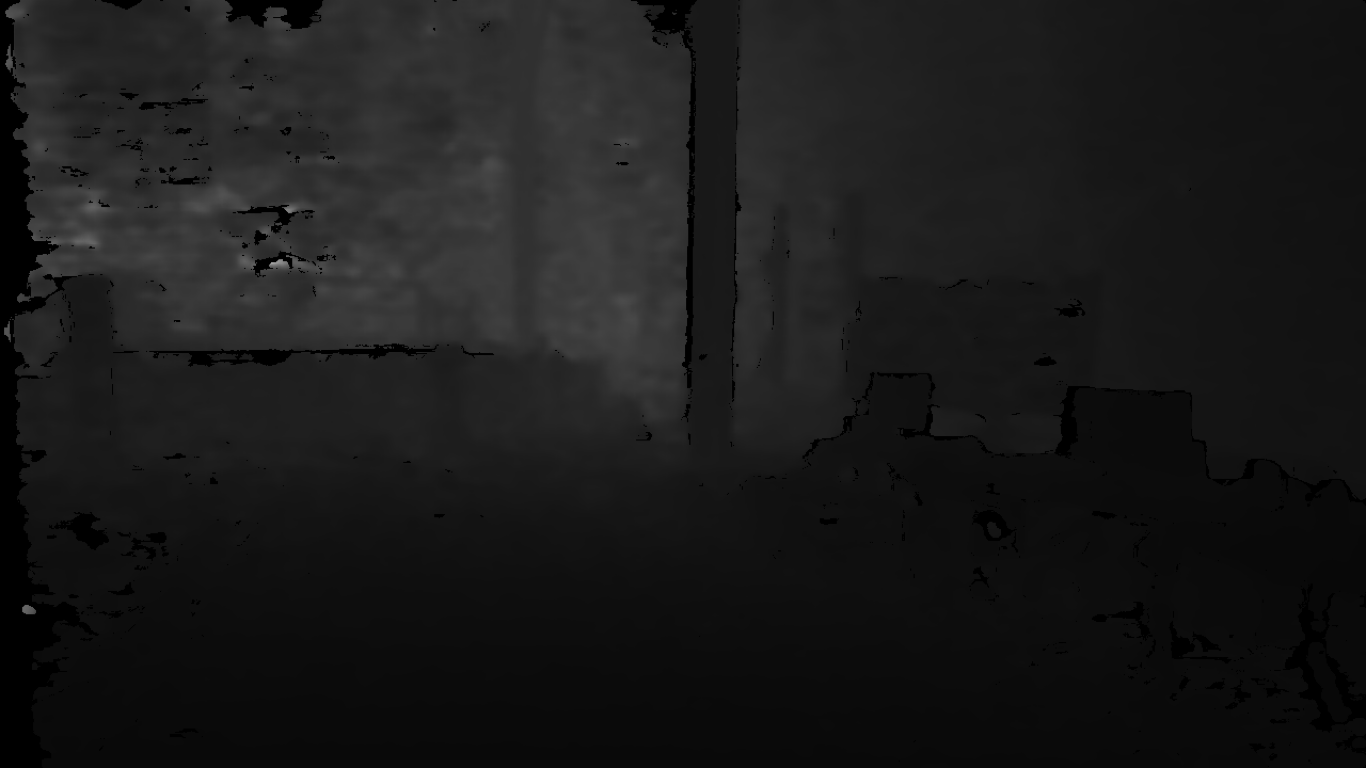
\includegraphics[width=.5\linewidth]{Pictures/mapping/vis_depth.png}
    \caption{2D segmentation and Depth image}
    \label{fig:eg1}
\end{figure}
\textbf{Local Map Generation:}
In contrast, the local map generation follows a different protocol. Each segment in the camera frame is first transformed into the drone frame. The drone's pose, estimated by the IMU, is then used to calculate the transformation matrix from the drone frame to the world frame. This step is crucial for estimating the 3D centroid of each segment in the world frame. The local map segments, like the global map, retain information about their 2D image pixel center and label, which is vital for subsequent matching processes and the integration of local map data into the global map framework.

\textbf{Estimating the Transformation Matrix with IMU Data:}
IMU data plays a pivotal role in estimating the drone's current pose in the world frame, particularly for the local map. The IMU's sensors, including accelerometers and gyroscopes, provide raw data on the drone's linear acceleration and angular velocity. By integrating this data over time, an estimation of the drone's velocity, orientation, and position relative to its initial state is achieved. This transformation matrix provided by the IMU data is instrumental in estimating the pose of segments in the world frame.

\textbf{Limitations in Local Map Realization:}
Although the ideal scenario for local map generation would involve detecting segments across a wide range of distances, as illustrated in Figures \ref{fig:map1}, the current setup using a single RGB-D camera faces limitations. Specifically, the camera's range restricts detection to nearer segments, typically in darker shades of blue or red, as shown in Figure \ref{fig:pc_real}. This limitation highlights the need for equipment capable of longer-range perception for more comprehensive local mapping.

\begin{figure}[H]
    \centering
    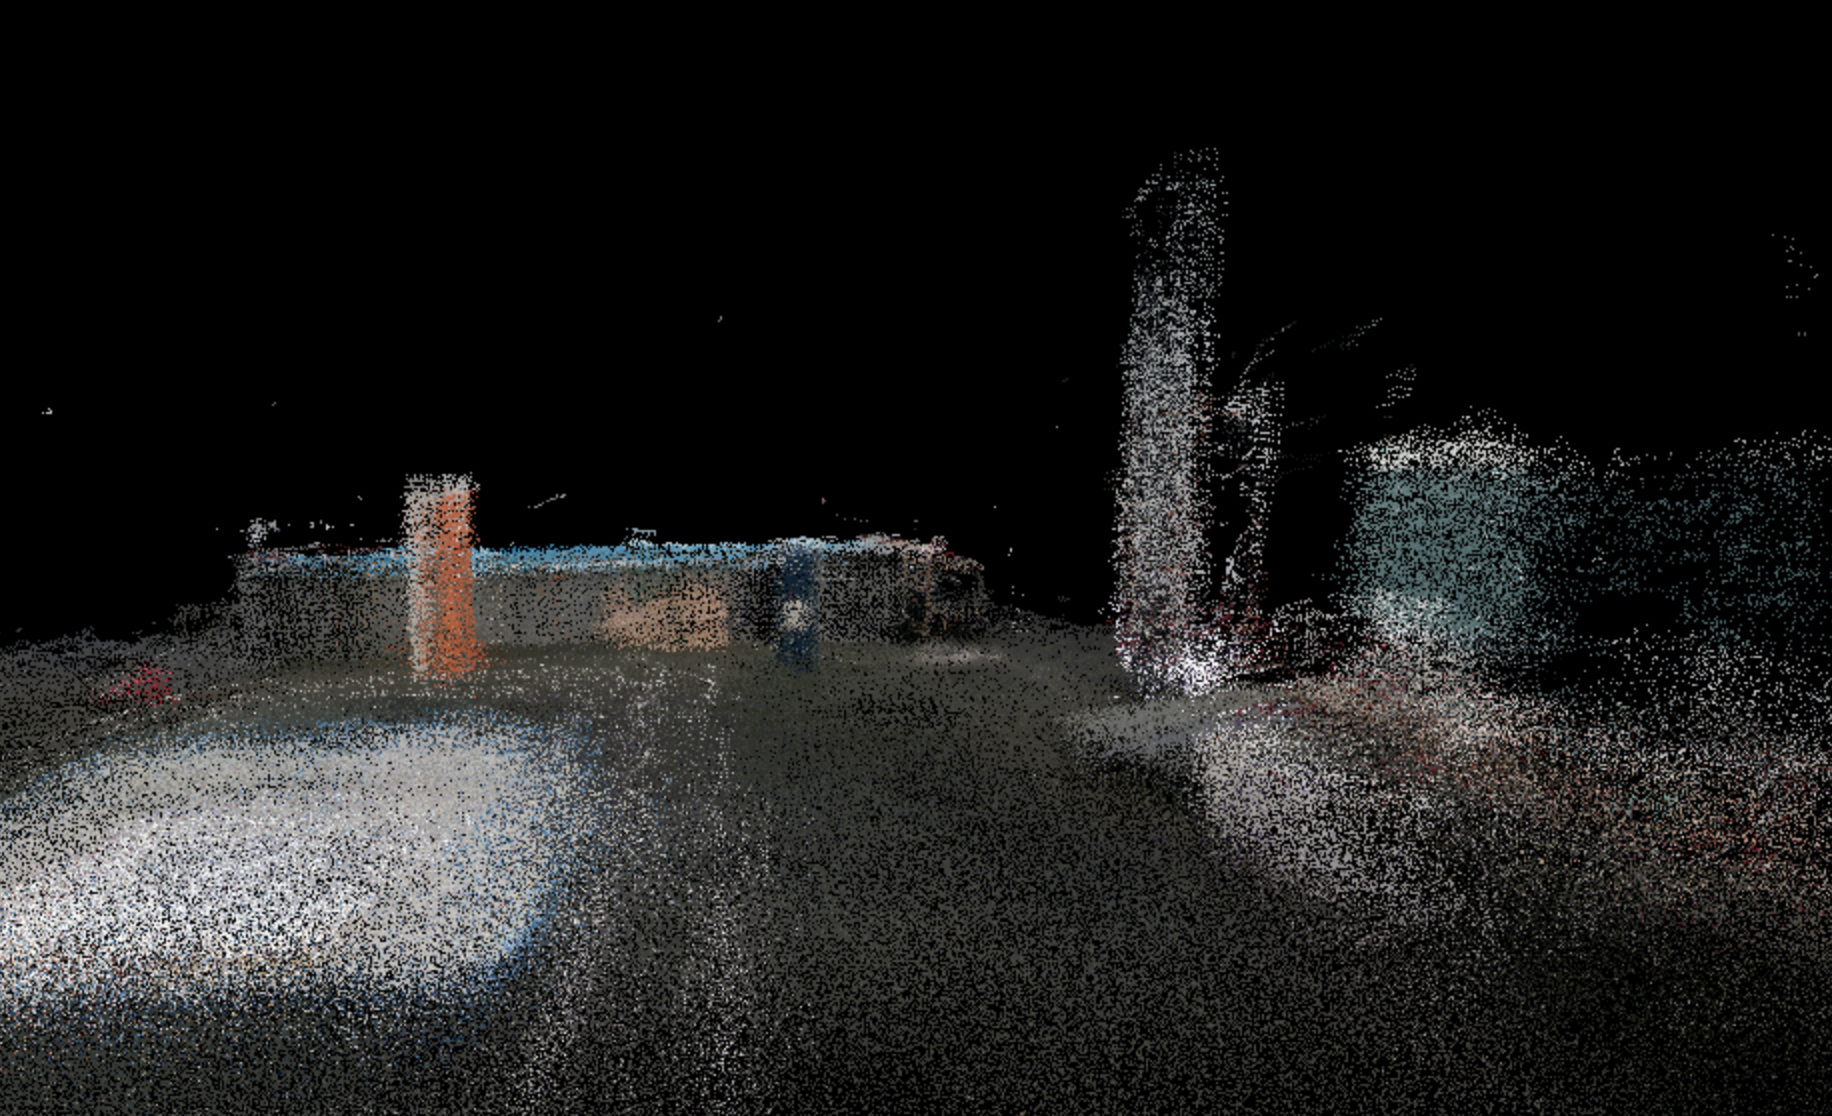
\includegraphics[width=.5\linewidth]
    {Pictures/mapping/vis_map1.png}\hfill
    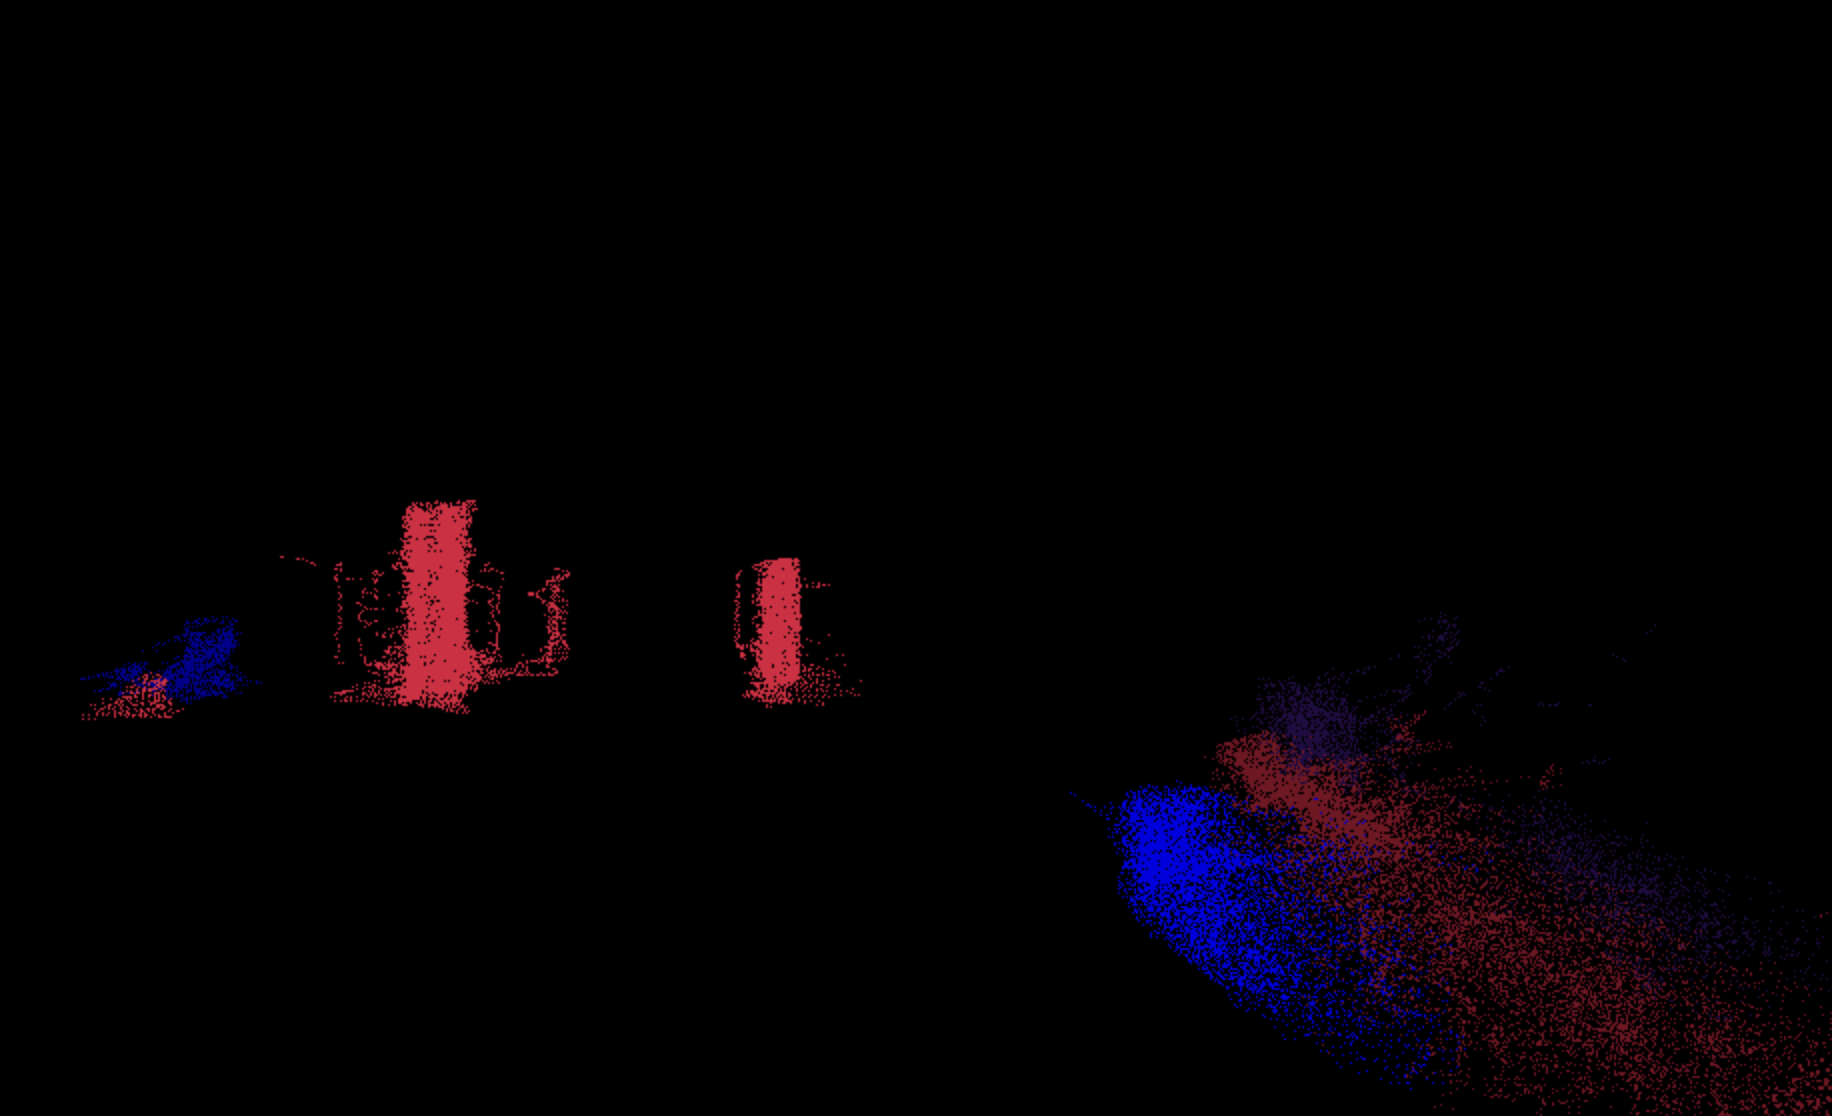
\includegraphics[width=.5\linewidth]{Pictures/mapping/vis_map2.png}
    \caption{Visualization of Frame in the Global Real Map and Semantic Map}
    \label{fig:map1}
\end{figure}

\begin{figure}[H]
    \centering
    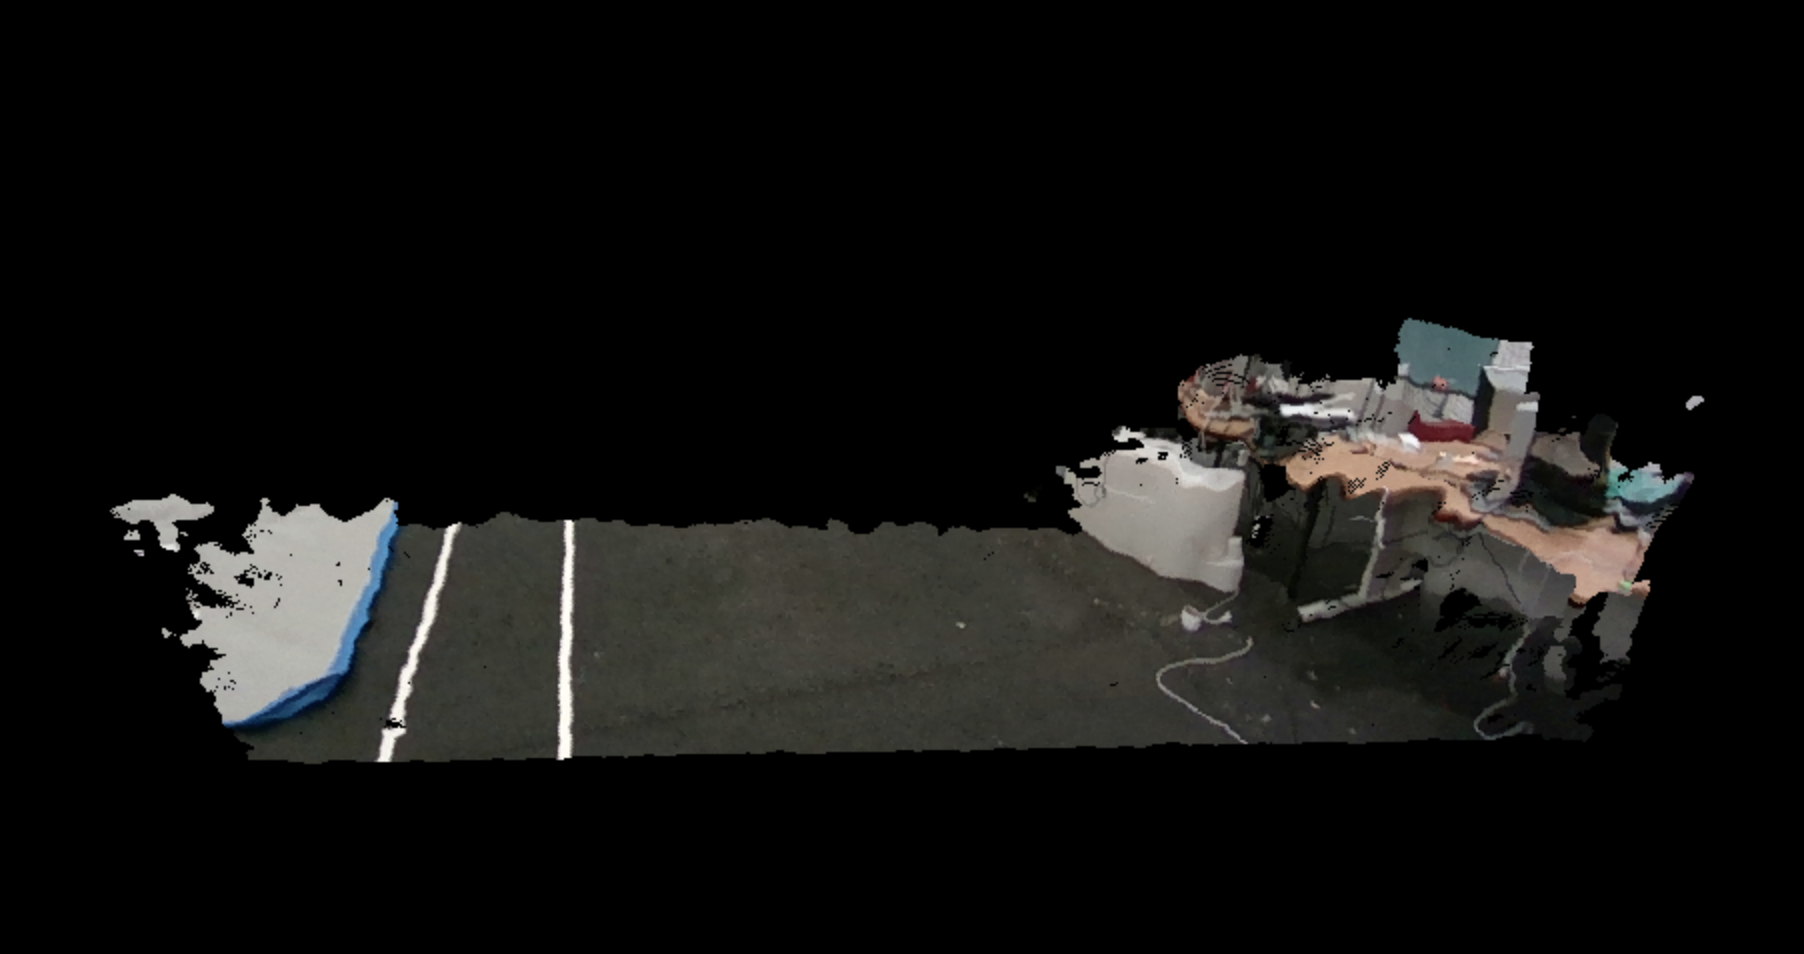
\includegraphics[width=.9\linewidth]{Pictures/mapping/vis_real.png}
    \caption{Local Point Cloud with RGB Information.}
    \label{fig:pc_real}

\textbf{Visualization of Segment Transformations:}
To provide a clear understanding of the transformation process, visualizations of local segments in both the camera frame and the world frame are presented. Left picture in Fig. \ref{fig:cam_vis} shows the segments as they appear in the camera frame, whereas right picture in Fig. \ref{fig:world_vis} displays these same segments transformed into the world frame. These visualizations underscore the transformation process, highlighting the transition of data from the drone's perspective to a global context, which is essential for accurate map generation and spatial analysis.

\end{figure}
\begin{figure}[H]
    \centering
    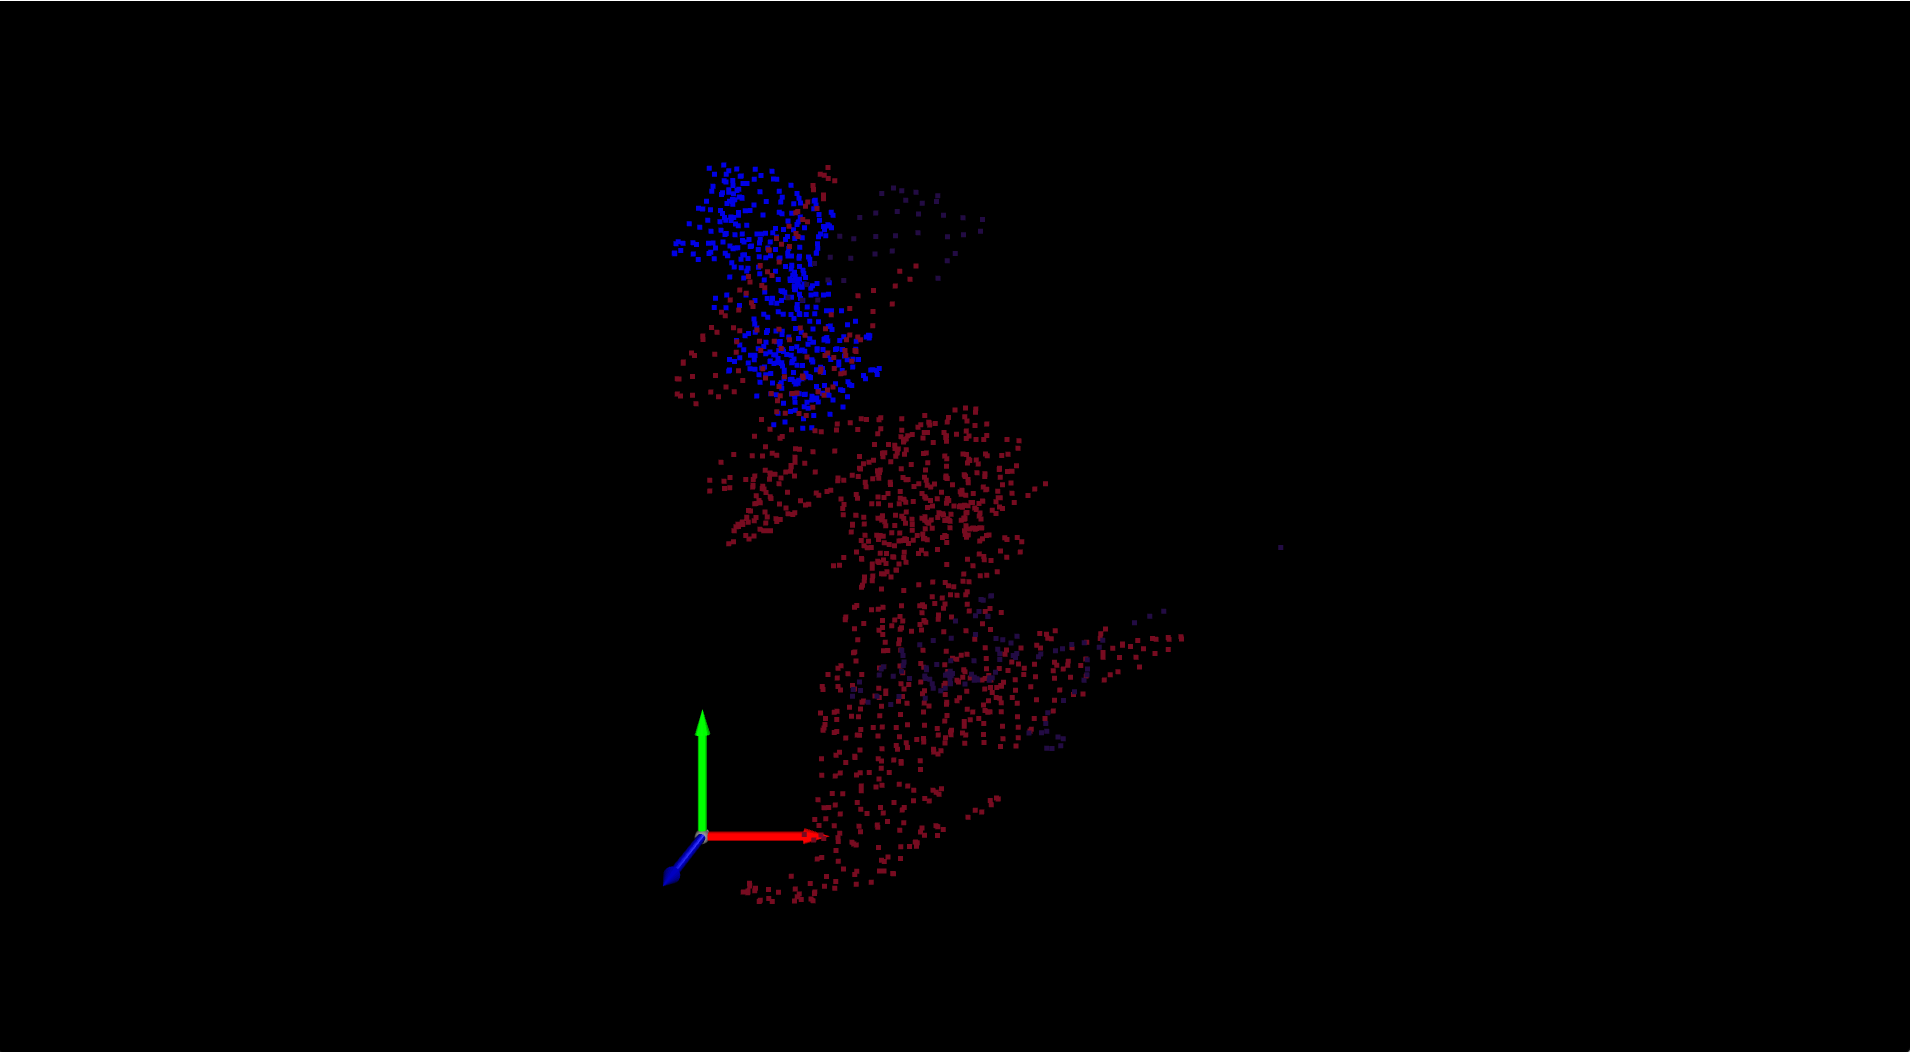
\includegraphics[width=.5\linewidth]{Pictures/mapping/vis_camframe.png}\hfill
    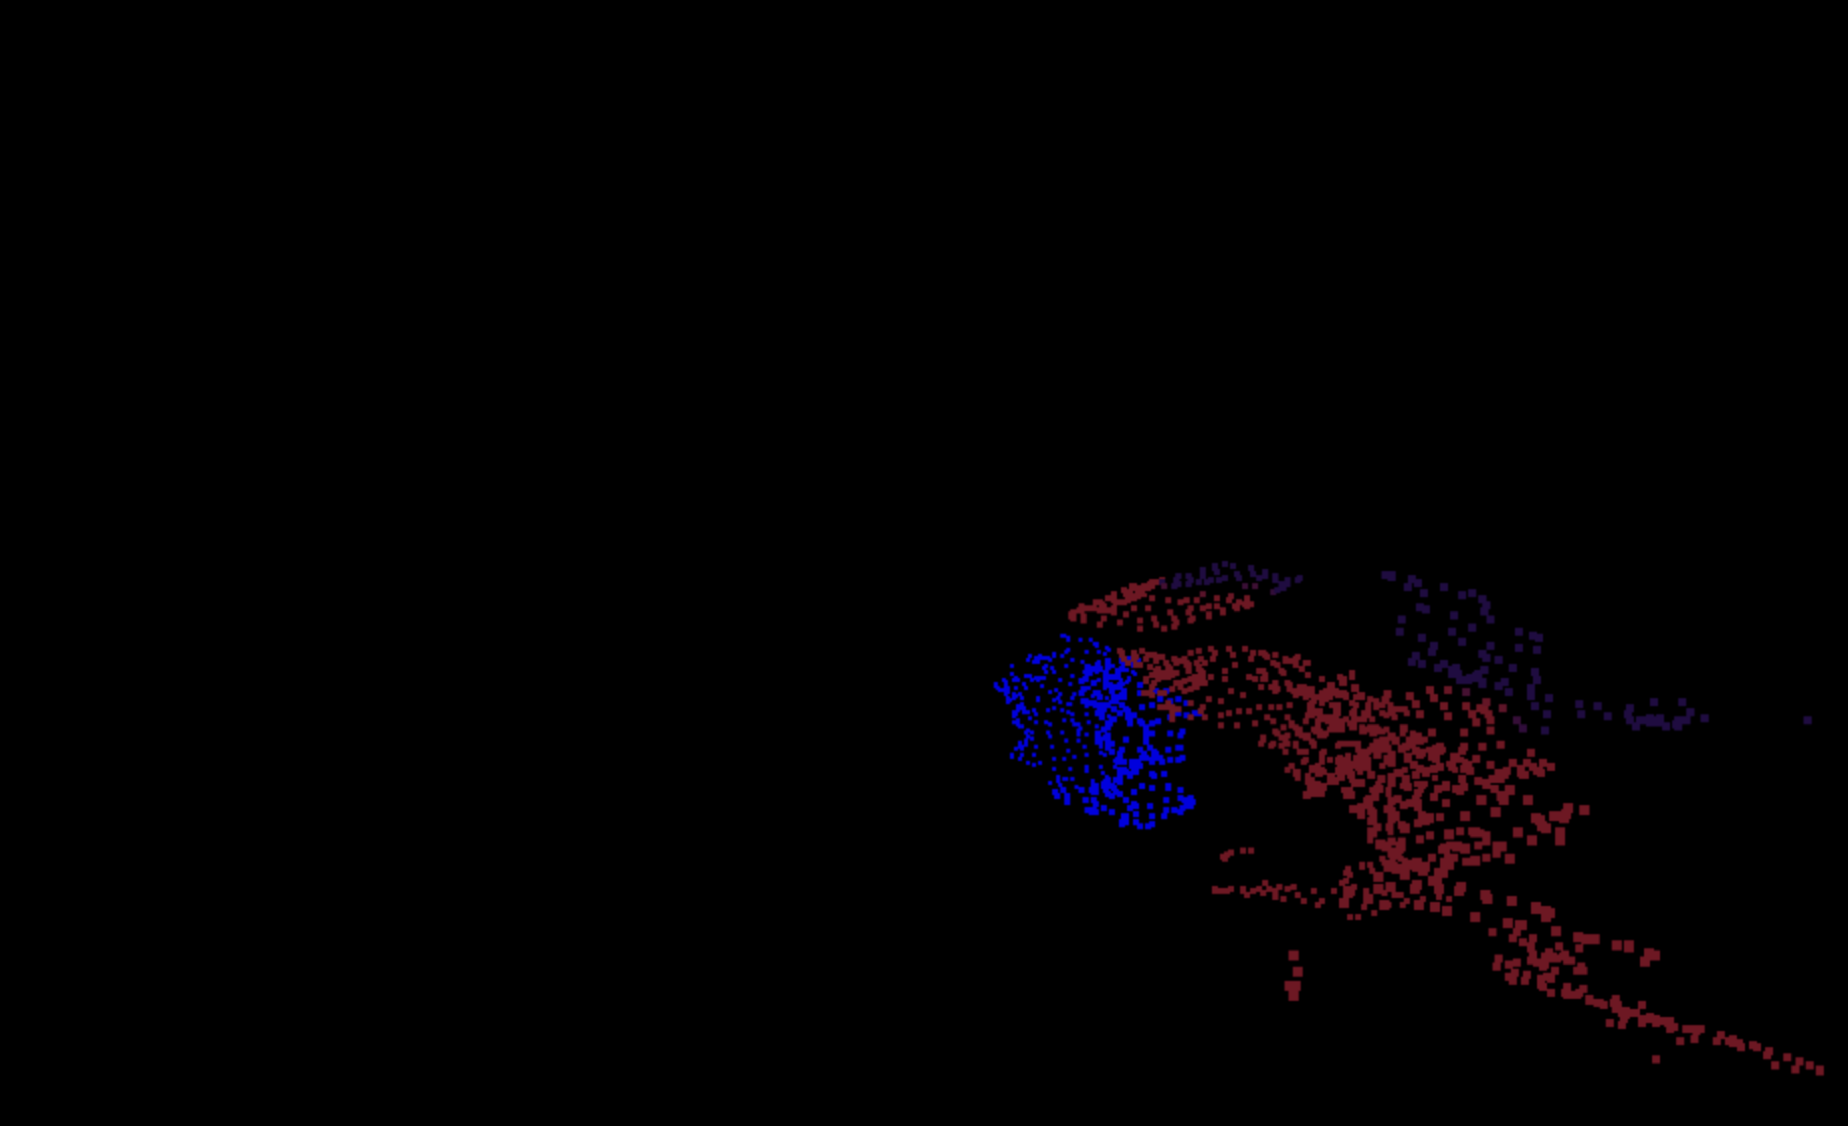
\includegraphics[width=.4\linewidth]{Pictures/mapping/vis_world.png}
    \caption{Local Segment in Camera Frame and World Frame.}
    \label{fig:cam_vis}
\end{figure}

\section{Methodology for Real-Time Pose Estimation with IMU}

Pose estimation plays a pivotal role in the field of \acrshort{uavs}, enabling critical capabilities such as autonomous navigation, obstacle avoidance, and dynamic interaction with the environment. The real-time estimation of the UAV's position and orientation, referred to as pose, is fundamental for effective operational control and autonomy.

\subsection{Challenges in Real-Time Pose Estimation} 
Real-time pose estimation in dynamic environments presents several challenges. These include the need for high accuracy and low latency in the face of limited computational resources, environmental variability, and the inherent noise in sensor data.

\subsection{Overview of the Approach} 
This section presents the approach to real-time pose estimation for UAVs, leveraging data from Inertial Measurement Units (IMUs). The method focuses on estimating the drone's position (x, y, z) and orientation (roll, pitch, yaw) in real-time, using sensor fusion and integration techniques. IMUs measure linear accelerations and angular velocities. The accelerometers measure specific force (acceleration) along three orthogonal axes, while gyroscopes measure angular velocity around these axes. These measurements are the primary inputs for estimating the UAV's pose.

\textit{Data Acquisition and Preprocessing} IMUs measure linear accelerations and angular velocities. The accelerometers measure specific force (acceleration) along three orthogonal axes, while gyroscopes measure angular velocity around these axes. These measurements are the primary inputs for estimating the UAV's pose. Preprocessing steps are crucial in enhancing the accuracy of this data. These steps include:
\begin{itemize}
    \item Bias Removal: Both accelerometers and gyroscopes exhibit biases that can significantly affect measurement accuracy. These biases are subtracted from the raw measurements to enhance data fidelity.
    \item Noise Filtering: IMU data is susceptible to noise, often necessitating the application of filtering techniques to obtain cleaner signals.
\end{itemize}

\textit{Transformation and Integration Techniques} The transformation from the IMU's coordinate system to the drone's coordinate system is achieved using transformation matrix:

\[ T_{ID} = \begin{pmatrix} R_{ID} & \vec{t}_{ID} \\ 0 & 1 \end{pmatrix} \].

Here translation vector is emply and this matrix accounts for the orientation differences between the IMU and the drone's frame of reference.
The transformation matrix from drone frame to world frame is:
\[ T_{DW} = \begin{pmatrix} R_{DW} & \vec{t}_{DW} \\ 0 & 1 \end{pmatrix} \]

Unlike the $T_{ID}$ which is predefined by user and has fix value, $T_{DW}$ needs to be calculated by using gyro to update orientation and the $R_{DW}$ and use the updated $R_{DW}$ to update velocity and position by applying the ration matrix to acceleration.

\textit{Orientation Estimation} The orientation of the UAV is estimated by integrating the angular velocity measurements from the gyroscopes. The integration process involves computing the incremental changes in orientation over time, described by the following equation:
\begin{equation}
    \Delta \text{orientation} = \text{gyro} \times dt
\end{equation}
where \(\text{gyro}\) is the angular velocity vector and \(dt\) is the time interval. The drone's orientation in terms of roll, pitch, and yaw is updated incrementally using these calculations.

\textit{Position Estimation} The position of the UAV is estimated by integrating the acceleration data to compute velocity and subsequently position. The accelerations, after being corrected for gravitational effects, are integrated to obtain velocity:
\begin{equation}
    \text{velocity}_{t} = \text{velocity}_{t-1} + \text{acceleration} \times dt
\end{equation}
The velocity is then integrated to calculate the position:
\begin{equation}
    \text{position}_{t} = \text{position}_{t-1} + \text{velocity}_{t} \times dt + 0.5 \times \text{acceleration} \times dt^2
\end{equation}

This method provides a comprehensive framework for real-time pose estimation using IMU data, which is essential for the dynamic and autonomous operation of UAVs.


\subsection{Mathematical Formulation of IMU-Based Pose Estimation}
The pose estimation algorithm integrates data from the Inertial Measurement Unit (IMU) to compute the orientation and position of the UAV in the world frame. The process involves several transformation and integration steps, abstractly formulated as follows:

\subsubsection{Coordinate Frame Definitions}

\begin{itemize}
    \item \( {f}_{I} \): The coordinate frame of the IMU.
    \item \( {f}_{D} \): The coordinate frame of the drone.
    \item \( {f}_{W} \): The world coordinate frame.
\end{itemize}

\subsubsection{Transformation Matrix and Bias Correction}
The transformation from the IMU frame to the drone frame is defined by the rotation matrix \({R}_{ID} \):
\begin{equation}
    {R}_{ID} = \begin{bmatrix}
    0 & -1 & 0 \\
    -1 & 0 & 0 \\
    0 & 0 & -1 
    \end{bmatrix}
\end{equation}

Bias is removed from the IMU measurements as follows:
\begin{align}
    gyro_{bias} &= \begin{bmatrix} 0.0020178240054855253 \\ 0.0017592206368581425 \\ 0.0017427009552286577 \end{bmatrix}, \\
    {acc}_{bias} &= \begin{bmatrix} 0.28478655780245 \\ -0.024718655019298263 \\ -9.828971270850001 \end{bmatrix}, \\
    {acc}_{corrected} &= {acc} - {acc}_{bias}, \\
    {gyro}_{corrected} &= {gyro} - {gyro}_{bias}.
\end{align}

\subsubsection{Orientation and Position Estimation}
The orientation estimation involves transforming the gyroscopic data from the IMU frame to the drone frame, and then to the world frame, followed by integration over time:
\begin{align}
    {gyro}_{W} &= {R}_{DW} \cdot {R}_{ID} \cdot {gyro}_{corrected}, \\
    {\Delta}_{orientation} &= {gyro}_{W} \times dt, \\
    {orientation}_{t} &= {orientation}_{t-1} + {\Delta}_{orientation}.
\end{align}

For position estimation, the acceleration data is similarly transformed and integrated:
\begin{align}
    {acc}_{W} &= {R}_{DW} \cdot {R}_{ID} \cdot {acc}_{corrected}, \\
    {\Delta}_{v} &= {acc}_{W} \times dt, \\
    {v}_{t} &= {v}_{t-1} + {\Delta}_{v}, \\
    {\Delta}_{position} &= {v}_{t-1} \times dt + \frac{1}{2} {acc}_{D} \times dt^2, \\
    {position}_{t} &= {position}_{t-1} + {\Delta}_{position}
\end{align}

where v, t and dt are velocity, current time and sampling time.
\subsection{Validation and Applications}
The accuracy and reliability of the pose estimation method are validated through various experiments and simulations. In IMU-based pose estimation for UAVs, two significant sources of error that affect accuracy and reliability are drift error and noise error\cite{imu_drift}.

Effective mitigation of drift and noise errors is crucial in IMU-based pose estimation systems. Approaches for addressing these errors include advanced sensor calibration techniques, implementation of filtering algorithms such as the Kalman filter, and sensor fusion methodologies that integrate data from vision-based pose estimation to enhance overall system accuracy and robustness.


\begin{figure}[H]
    \centering
    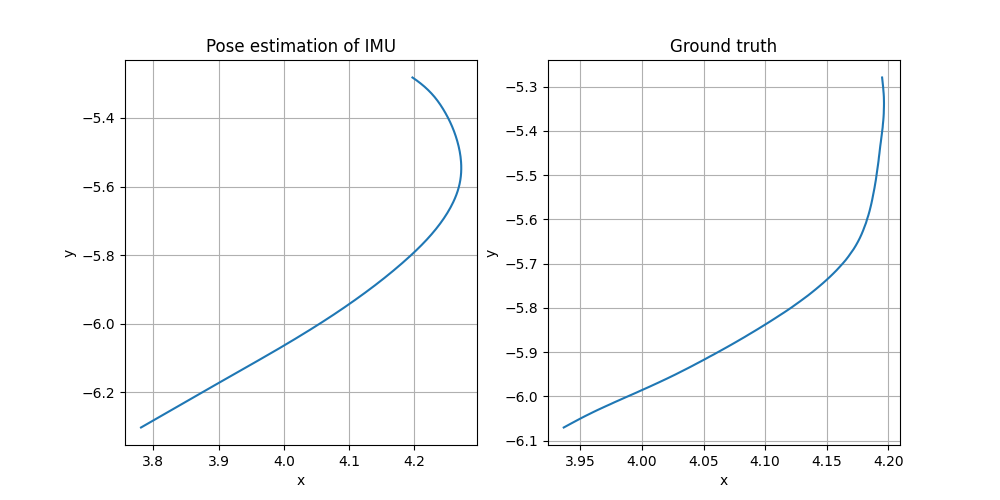
\includegraphics[width=.9\linewidth]{Pictures/pose_est/IMU_est_pose_xy.png}
    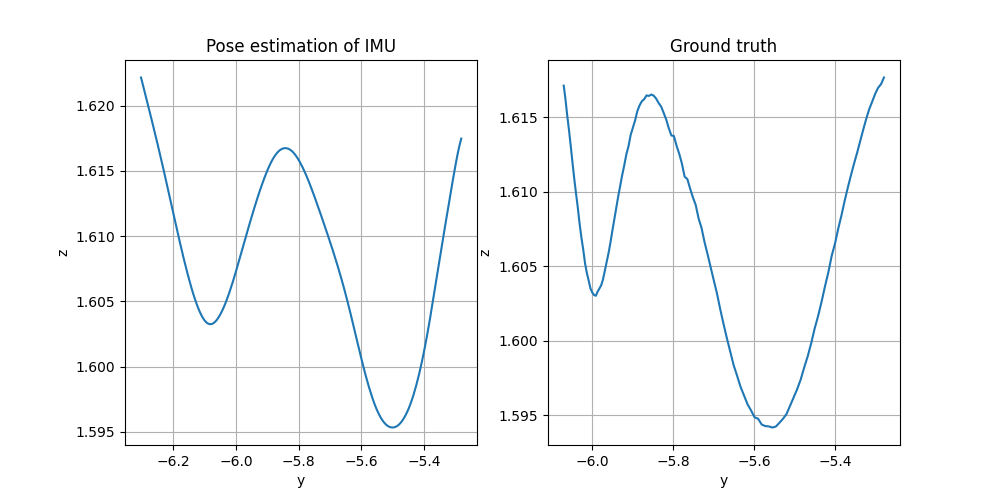
\includegraphics[width=.9\linewidth]{Pictures/pose_est/IMU_est_pose_yz.png}
    \caption{IMU-based Pose Estimation in 2D.}
    \label{fig:pos_est1}
\end{figure}

Figure \ref{fig:pos_est1} demonstrates that IMU-based pose estimation performs effectively over short intervals, such as those slightly exceeding one second. This short-term accuracy underscores the importance of precise calibration and bias correction in the estimation process. However, for real-time applications requiring continuous pose estimation, the limitations of IMU data become more apparent.

\begin{figure}[H]
    \centering
    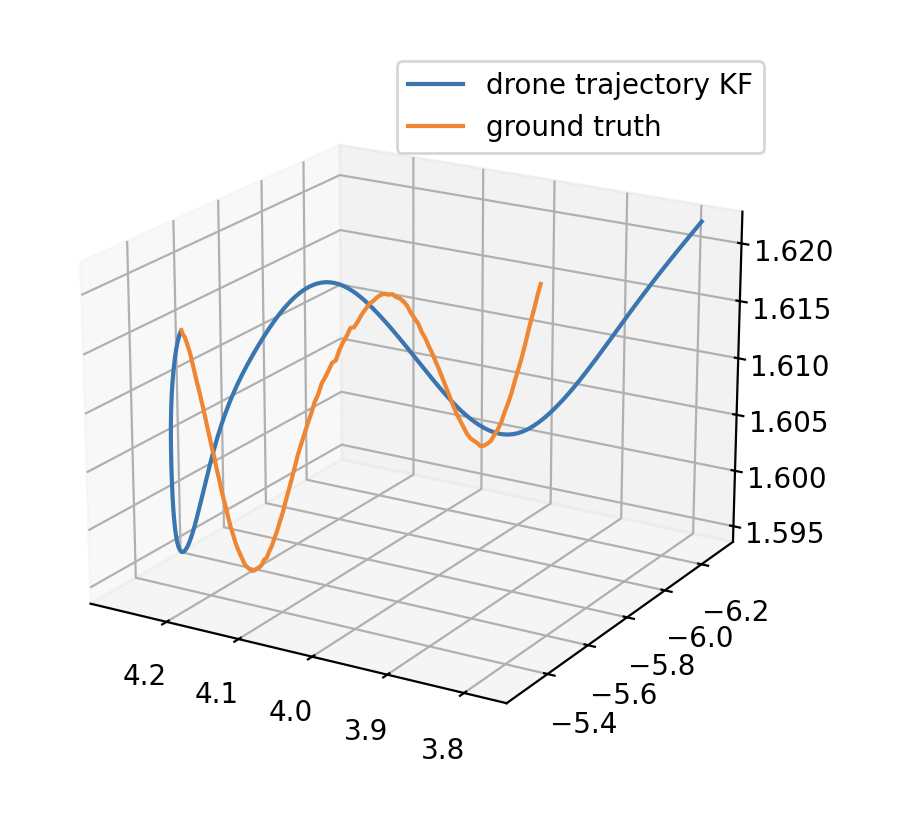
\includegraphics[width=.5\linewidth]{Pictures/pose_est/pose_est_IMU_3d.png}\hfill
    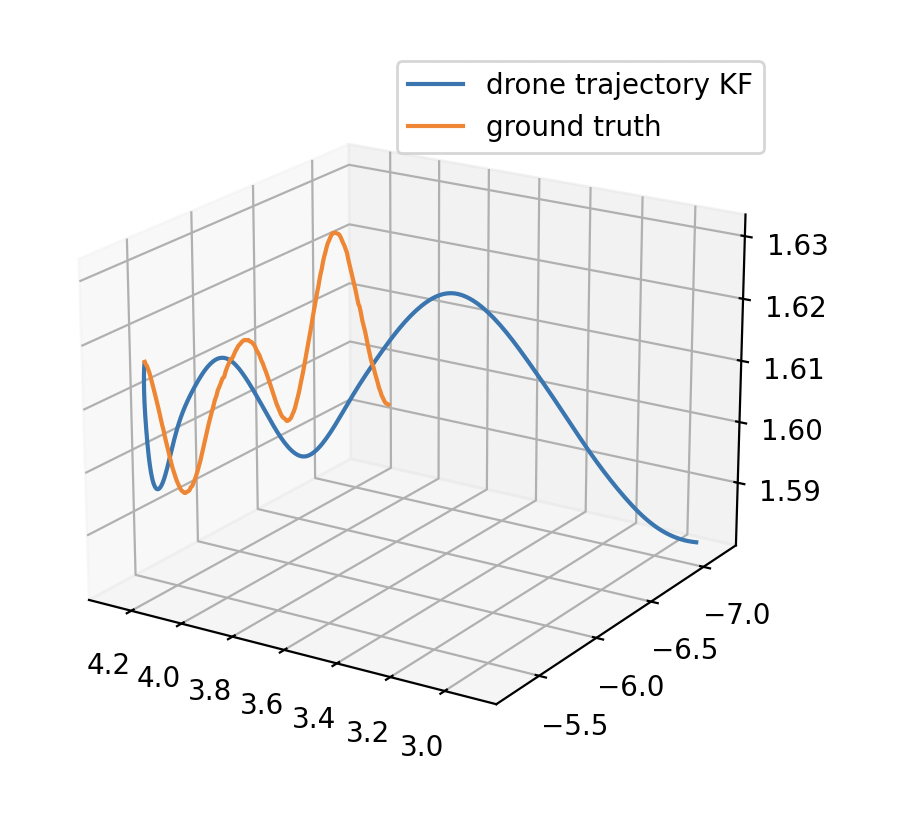
\includegraphics[width=.5\linewidth]{Pictures/pose_est/shift_error.png}
    \caption{IMU-based Pose Estimation in 3D.}
    \label{fig:pos_est2}
\end{figure}
As depicted in Figure \ref{fig:pos_est2}, while IMU data can provide a reasonable estimation in the short term, it is prone to accumulating errors over time. In scenarios requiring ongoing, real-time pose estimation, these errors can become significant. Shift error and noise error, in particular, tend to accumulate, leading to a level of inaccuracy that may be unacceptable for precise navigation tasks. This accumulation of errors is a critical challenge in utilizing IMU for long-term tracking and necessitates the consideration of additional data sources or correction methodologies to maintain accuracy in pose estimation over extended periods.

These findings highlight the inherent trade-offs in using IMU data for pose estimation: while useful for short-duration estimations due to its immediacy and relative simplicity, it lacks the long-term reliability required for sustained and precise navigation tasks. Therefore, for applications demanding continuous and accurate pose tracking, such as in advanced drone navigation or autonomous vehicle systems, it becomes necessary to either integrate additional sensing modalities or develop sophisticated algorithms to compensate for the IMU's limitations. This could involve the use of visual data or other sensor fusion techniques to correct and refine the pose estimates over time, ensuring sustained accuracy and reliability in real-world applications.



\section{Matching Strategy in a Prior Map}

Accurate localization in GNSS-denied environments is a significant challenge in autonomous navigation, necessitating advanced techniques in computer vision and sensor fusion. This section discusses the methodologies and algorithms employed for matching sensor-derived data with a pre-established map.

The proposed method combines gyroscopic and accelerometric data from IMUs with visual segment analysis. This involves extracting features from environmental landmarks, with a focus on segment-based visual data processing. Segments, which include descriptors, centroids, and labels, are extracted from the visual data and then matched against a prior map containing similar information for global segments.

The matching strategy encompasses several steps:

\textbf{IMU Data Processing}: The raw IMU data is processed to estimate real-time pose, addressing biases and noise typically associated with these sensors.

\textbf{Visual Data Segmentation}: Concurrently, visual data is segmented to obtain descriptors, labels, and estimated 3D centroids, along with 2D centers of segments.

\textbf{Data Fusion}: The IMU and visual data streams are fused, marking entries with labels like \texttt{'IMU'} or \texttt{'Visual'} to manage the differing streaming rates of the sensors. High-frequency IMU data is used for pose estimation and stored in an EKF. When lower-frequency (30Hz) visual data arrives, the estimated pose serves as a reference for generating the local map.

\textbf{Local Map Analysis}: The local map, along with descriptors, estimated 3D centroids, and labels, is analyzed using the KD-Trees algorithm for efficient nearest-neighbor searches. This step involves finding the top five matches within the prior map and retrieving the corresponding K-nearest neighbor (KNN) distances.

\textbf{Distance Calculation}: Euclidean distances between the pairs of centroids (both from the local and prior maps) are calculated.

\textbf{Combined Distance Evaluation}: A combined distance metric is computed, incorporating the KNN distance, Euclidean distance, and a score reflecting the label consistency. The segment with the smallest combined distance is identified as the match in the prior map.

This intricate process of matching segments in the local map to those in the prior map is pivotal for segment-based pose estimation. By accurately identifying corresponding segments, the system can effectively determine the device's location relative to known landmarks in the prior map. This approach is especially crucial in environments where traditional GNSS-based localization is unreliable or unavailable.

The integration of IMU and visual data, along with the sophisticated use of algorithms like KD-Trees for nearest-neighbor searches, exemplifies the advanced level of sensor fusion and data analysis required in modern autonomous navigation systems. This matching strategy not only enhances the accuracy of localization but also contributes to the overall robustness and reliability of the navigation system in dynamic and challenging environments.

The subsequent section will delve into how these matched segments are utilized for segment-based pose estimation, further advancing the capability of the system to navigate.

\section{Segment-based Pose Estimation}

Pose estimation, the process of determining the position and orientation of a device within a space, is crucial for various applications in robotics and autonomous navigation. Through the implementation of an \acrlong{ekf}, uncertainties in IMU sensor data is deal with segment-base measurement in this section.

The EKF is designed to fuse IMU data with visual information for real-time pose estimation. It maintains a state vector, potentially encompassing position, orientation, and velocity of the drone. It is configured with specific variances for these parameters, reflecting the characteristics and sensor noise of the sensor in use.

The EKF operates by predicting the next state of the system based on the current state and control inputs derived from the IMU data. It then integrates the visual data, involving the position and possible orientation information extracted from the segmented visual data. This integration is achieved through a measurement update step, where the filter combines the predicted state with the new measurements to produce an updated estimate of the drone's pose.

Result of visual pose estimation  will differ when the number of valid segments in visual data is lower than 4, which means there are not enough segments to measure pose by utilizing PnP method. In this scenario, only position will be measured and used to updates state in EKF. When there are more than 4 segments detected, pose can be estimated by using PnP method, and more segments detected, more accurate the estimation would be. 

The mathematical backbone of the EKF involves formulating both a state transition model and a measurement model. The state transition model predicts the system's future state, considering the dynamics of movement and sensor inputs. The measurement model, on the other hand, relates the actual sensor measurements to the predicted state. Through a series of update and prediction steps, the EKF continuously refines its estimate of the device's pose, minimizing the overall uncertainty by balancing the predictions with new sensor inputs. This process is crucial for achieving accurate and reliable pose estimation in dynamic environments.


\section{Evaluation of Sensor Fusion}


\begin{figure}[H]
    \centering
    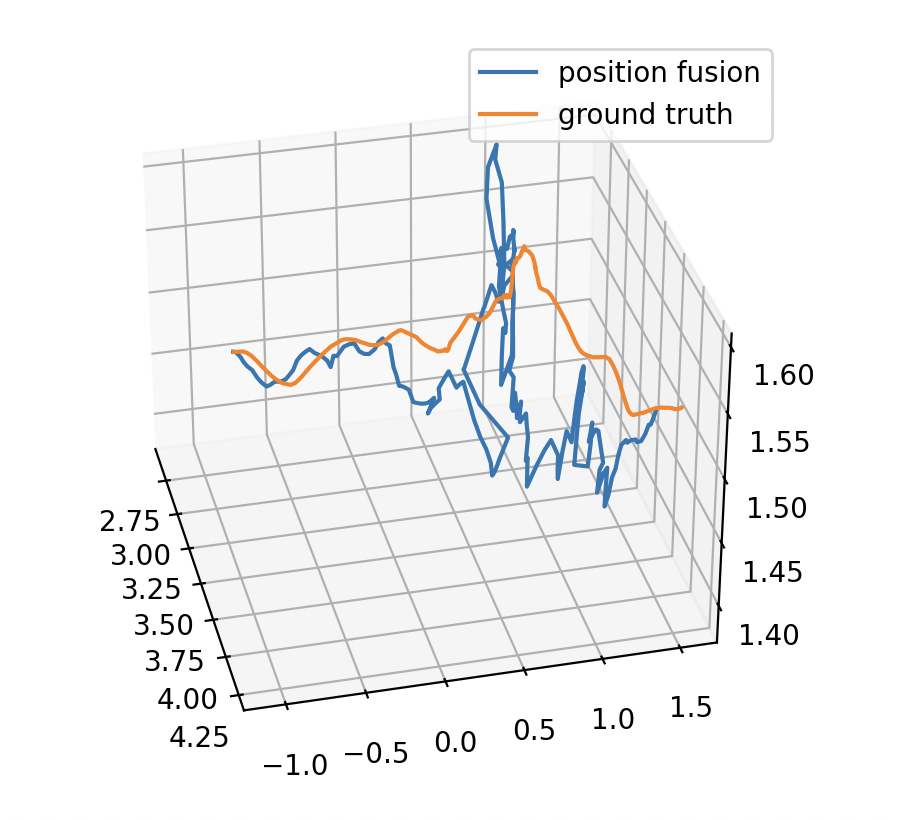
\includegraphics[width=.5\linewidth]{Pictures/sensor_fusion/10s_3d_fine.png}\hfill
    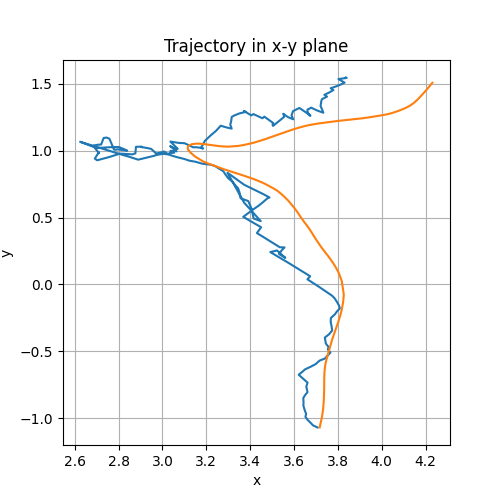
\includegraphics[width=.5\linewidth]{Pictures/sensor_fusion/xy_gt_10s_2.png}
    \caption{Comparison in 3D and Comparison in x-y Plane.}
    \label{fig:sensor_fusion_3_1}
\end{figure}

\begin{figure}
    \centering
    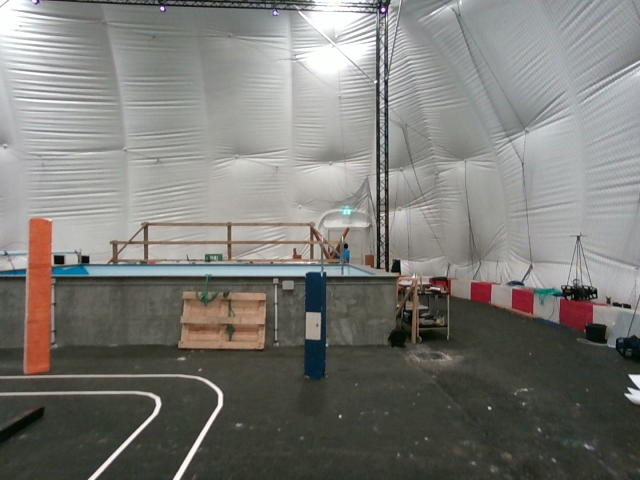
\includegraphics[width=.5\linewidth]{Pictures/sensor_fusion/rgb_1701886823.3972387.png}\hfill
    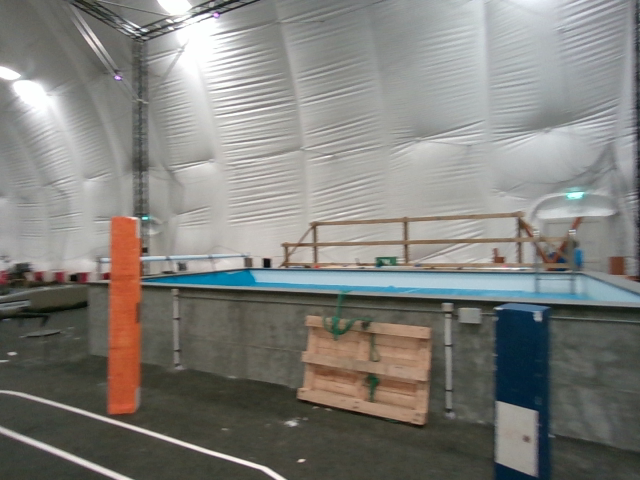
\includegraphics[width=.5\linewidth]{Pictures/sensor_fusion/rgb_1701886826.5639899.png}\hfill
    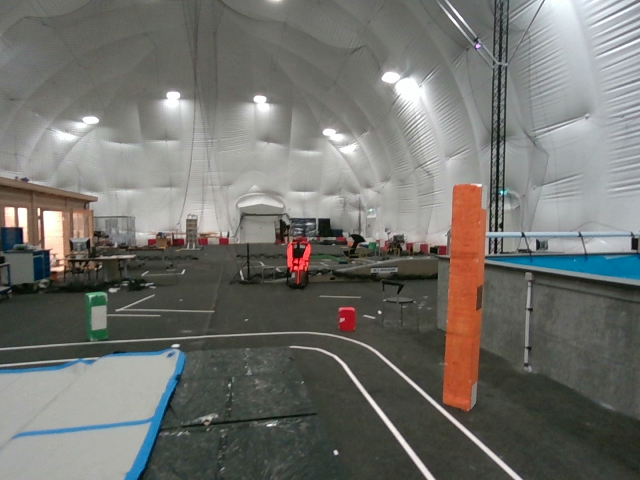
\includegraphics[width=.5\linewidth]{Pictures/sensor_fusion/rgb_1701886828.6657953.png}\hfill
    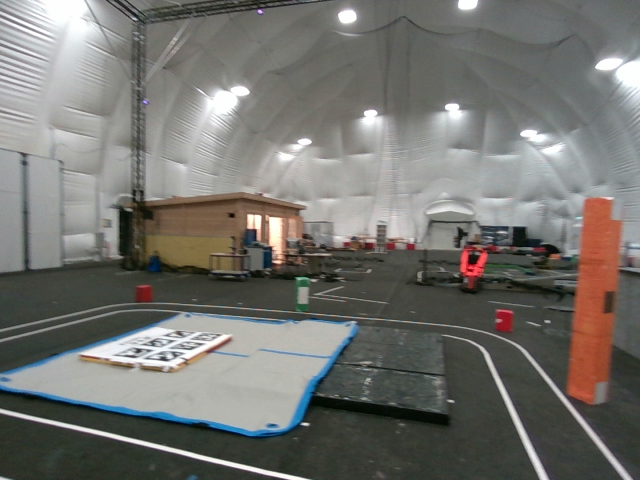
\includegraphics[width=.5\linewidth]{Pictures/sensor_fusion/rgb_1701886831.6306818.png}
    \caption{Visualization of Moving in 10 Seconds.}
    \label{fig:sensor_fusion_3_2}
\end{figure}

\begin{figure}[H]
    \centering
    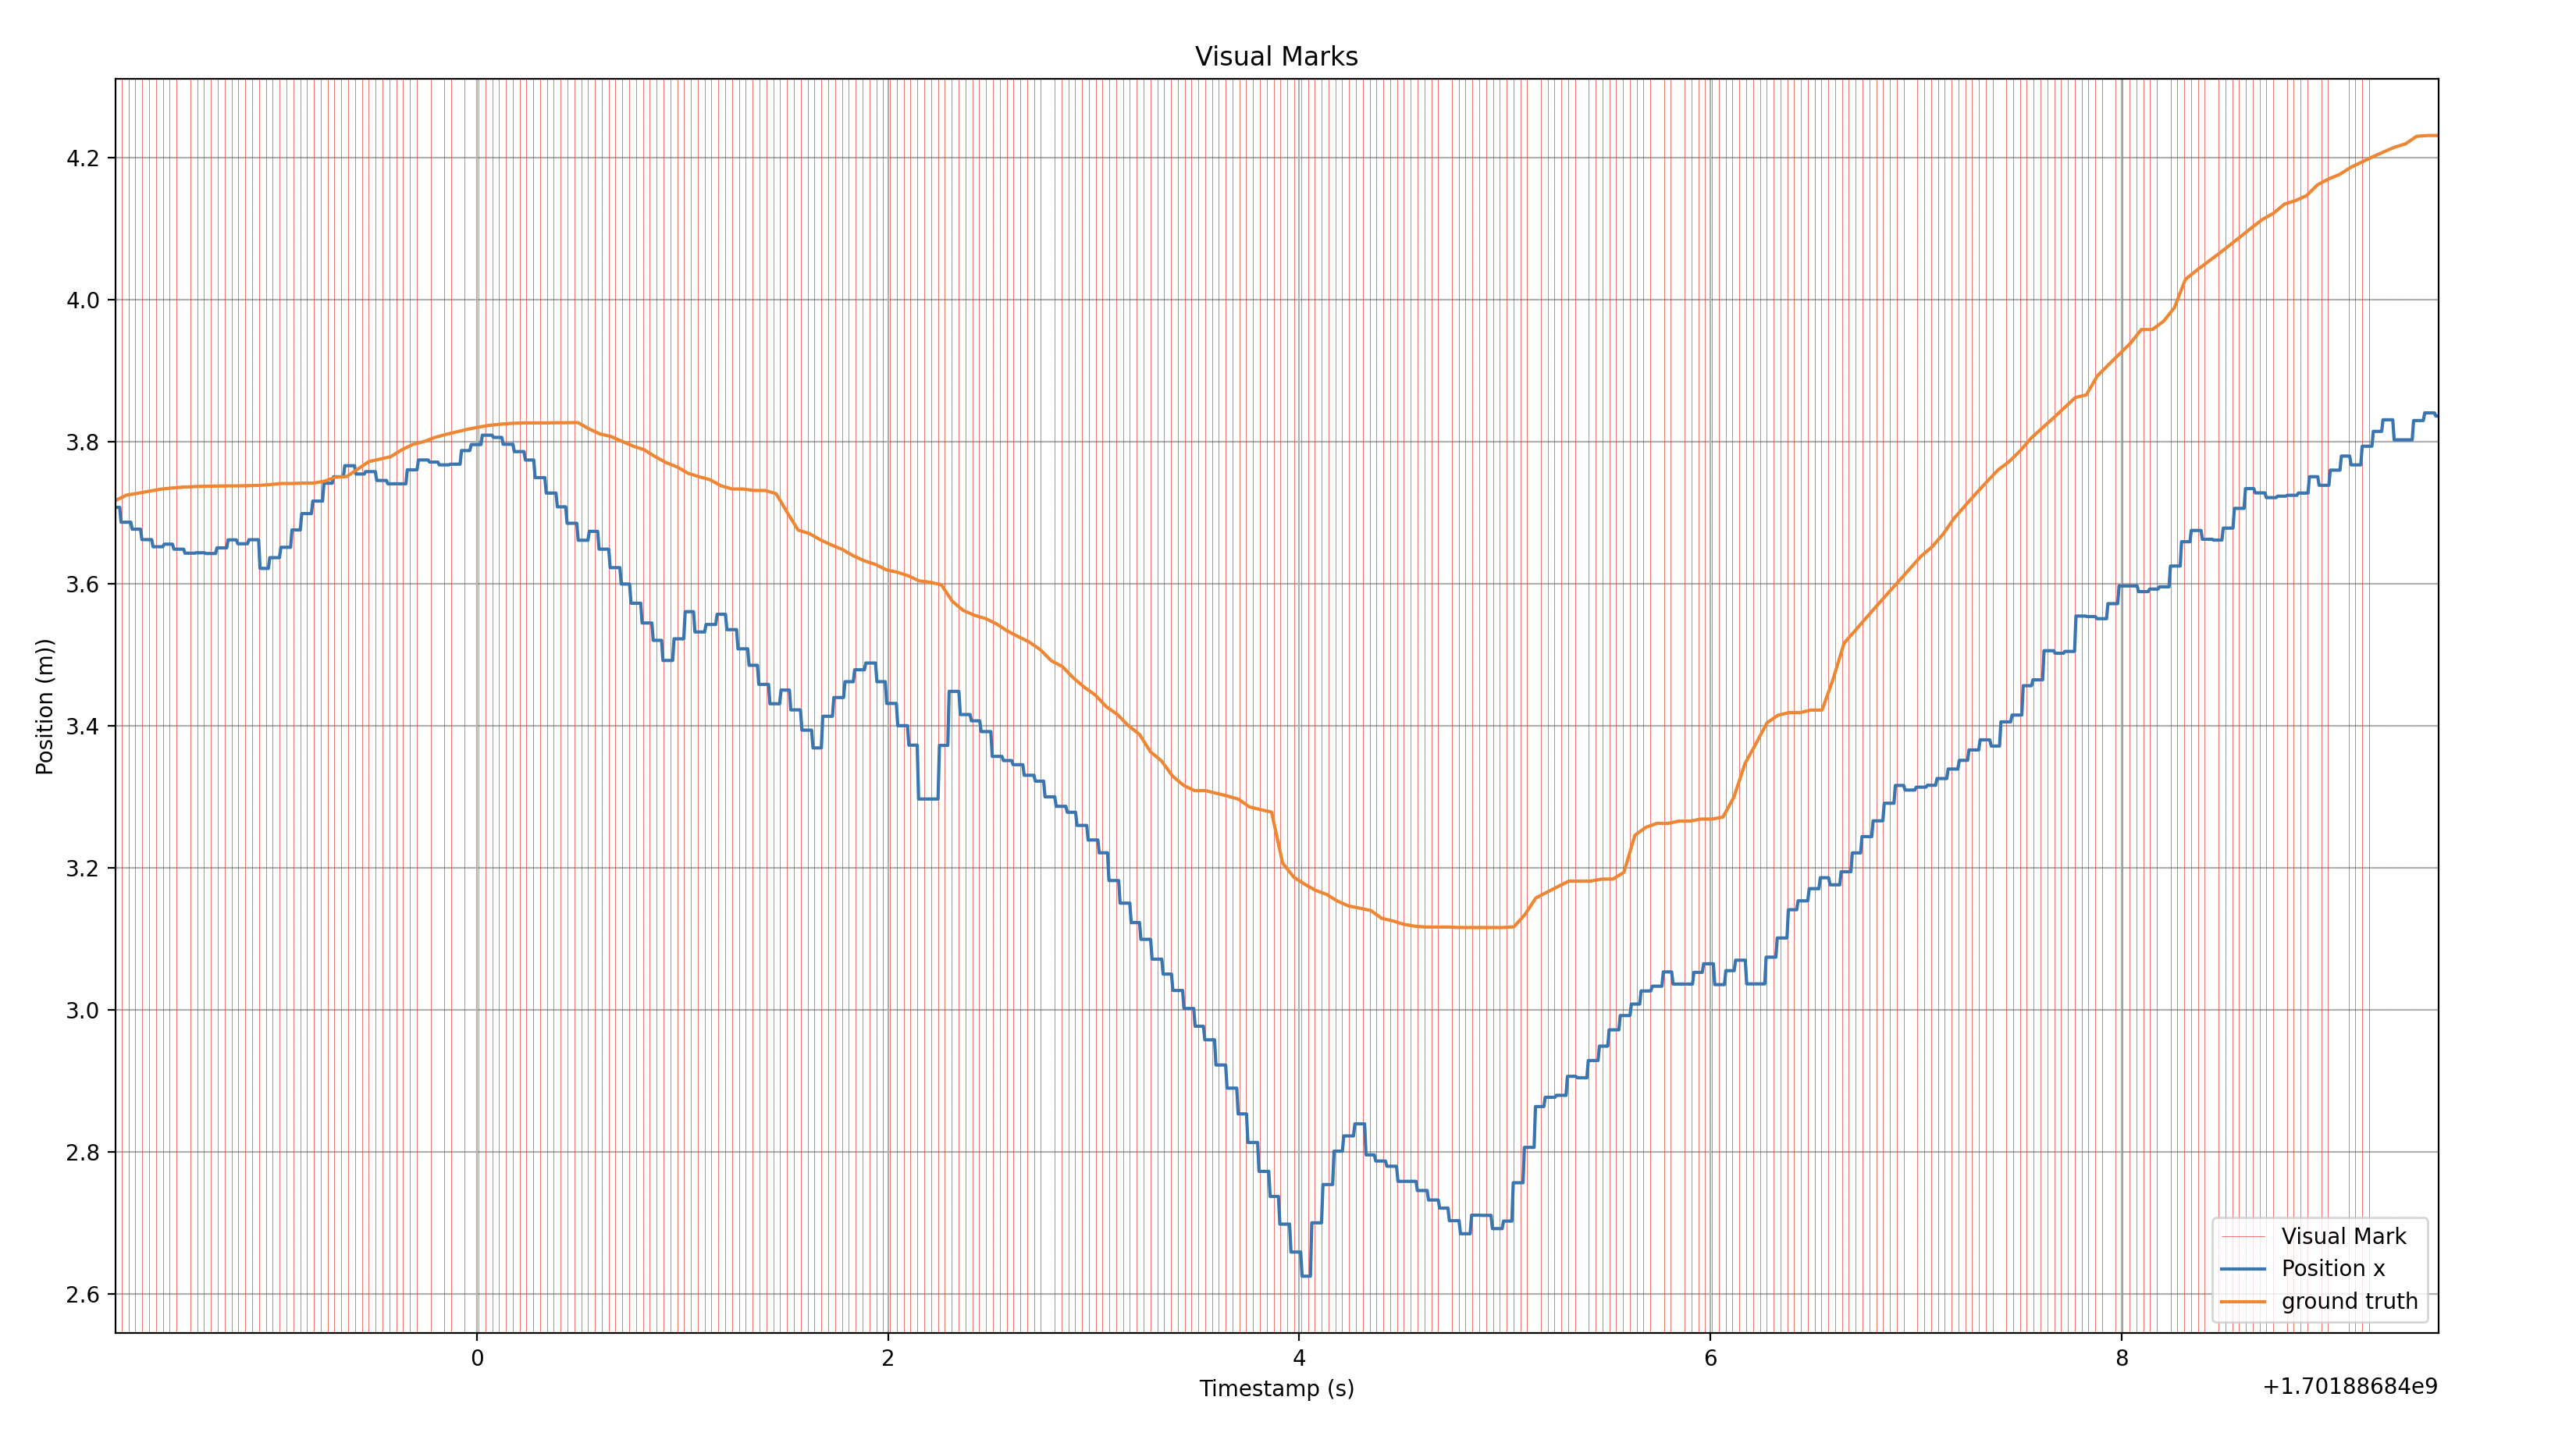
\includegraphics[width=.8\linewidth]{Pictures/sensor_fusion/Screenshot 2024-01-14 at 23.17.01.png}\hfill
    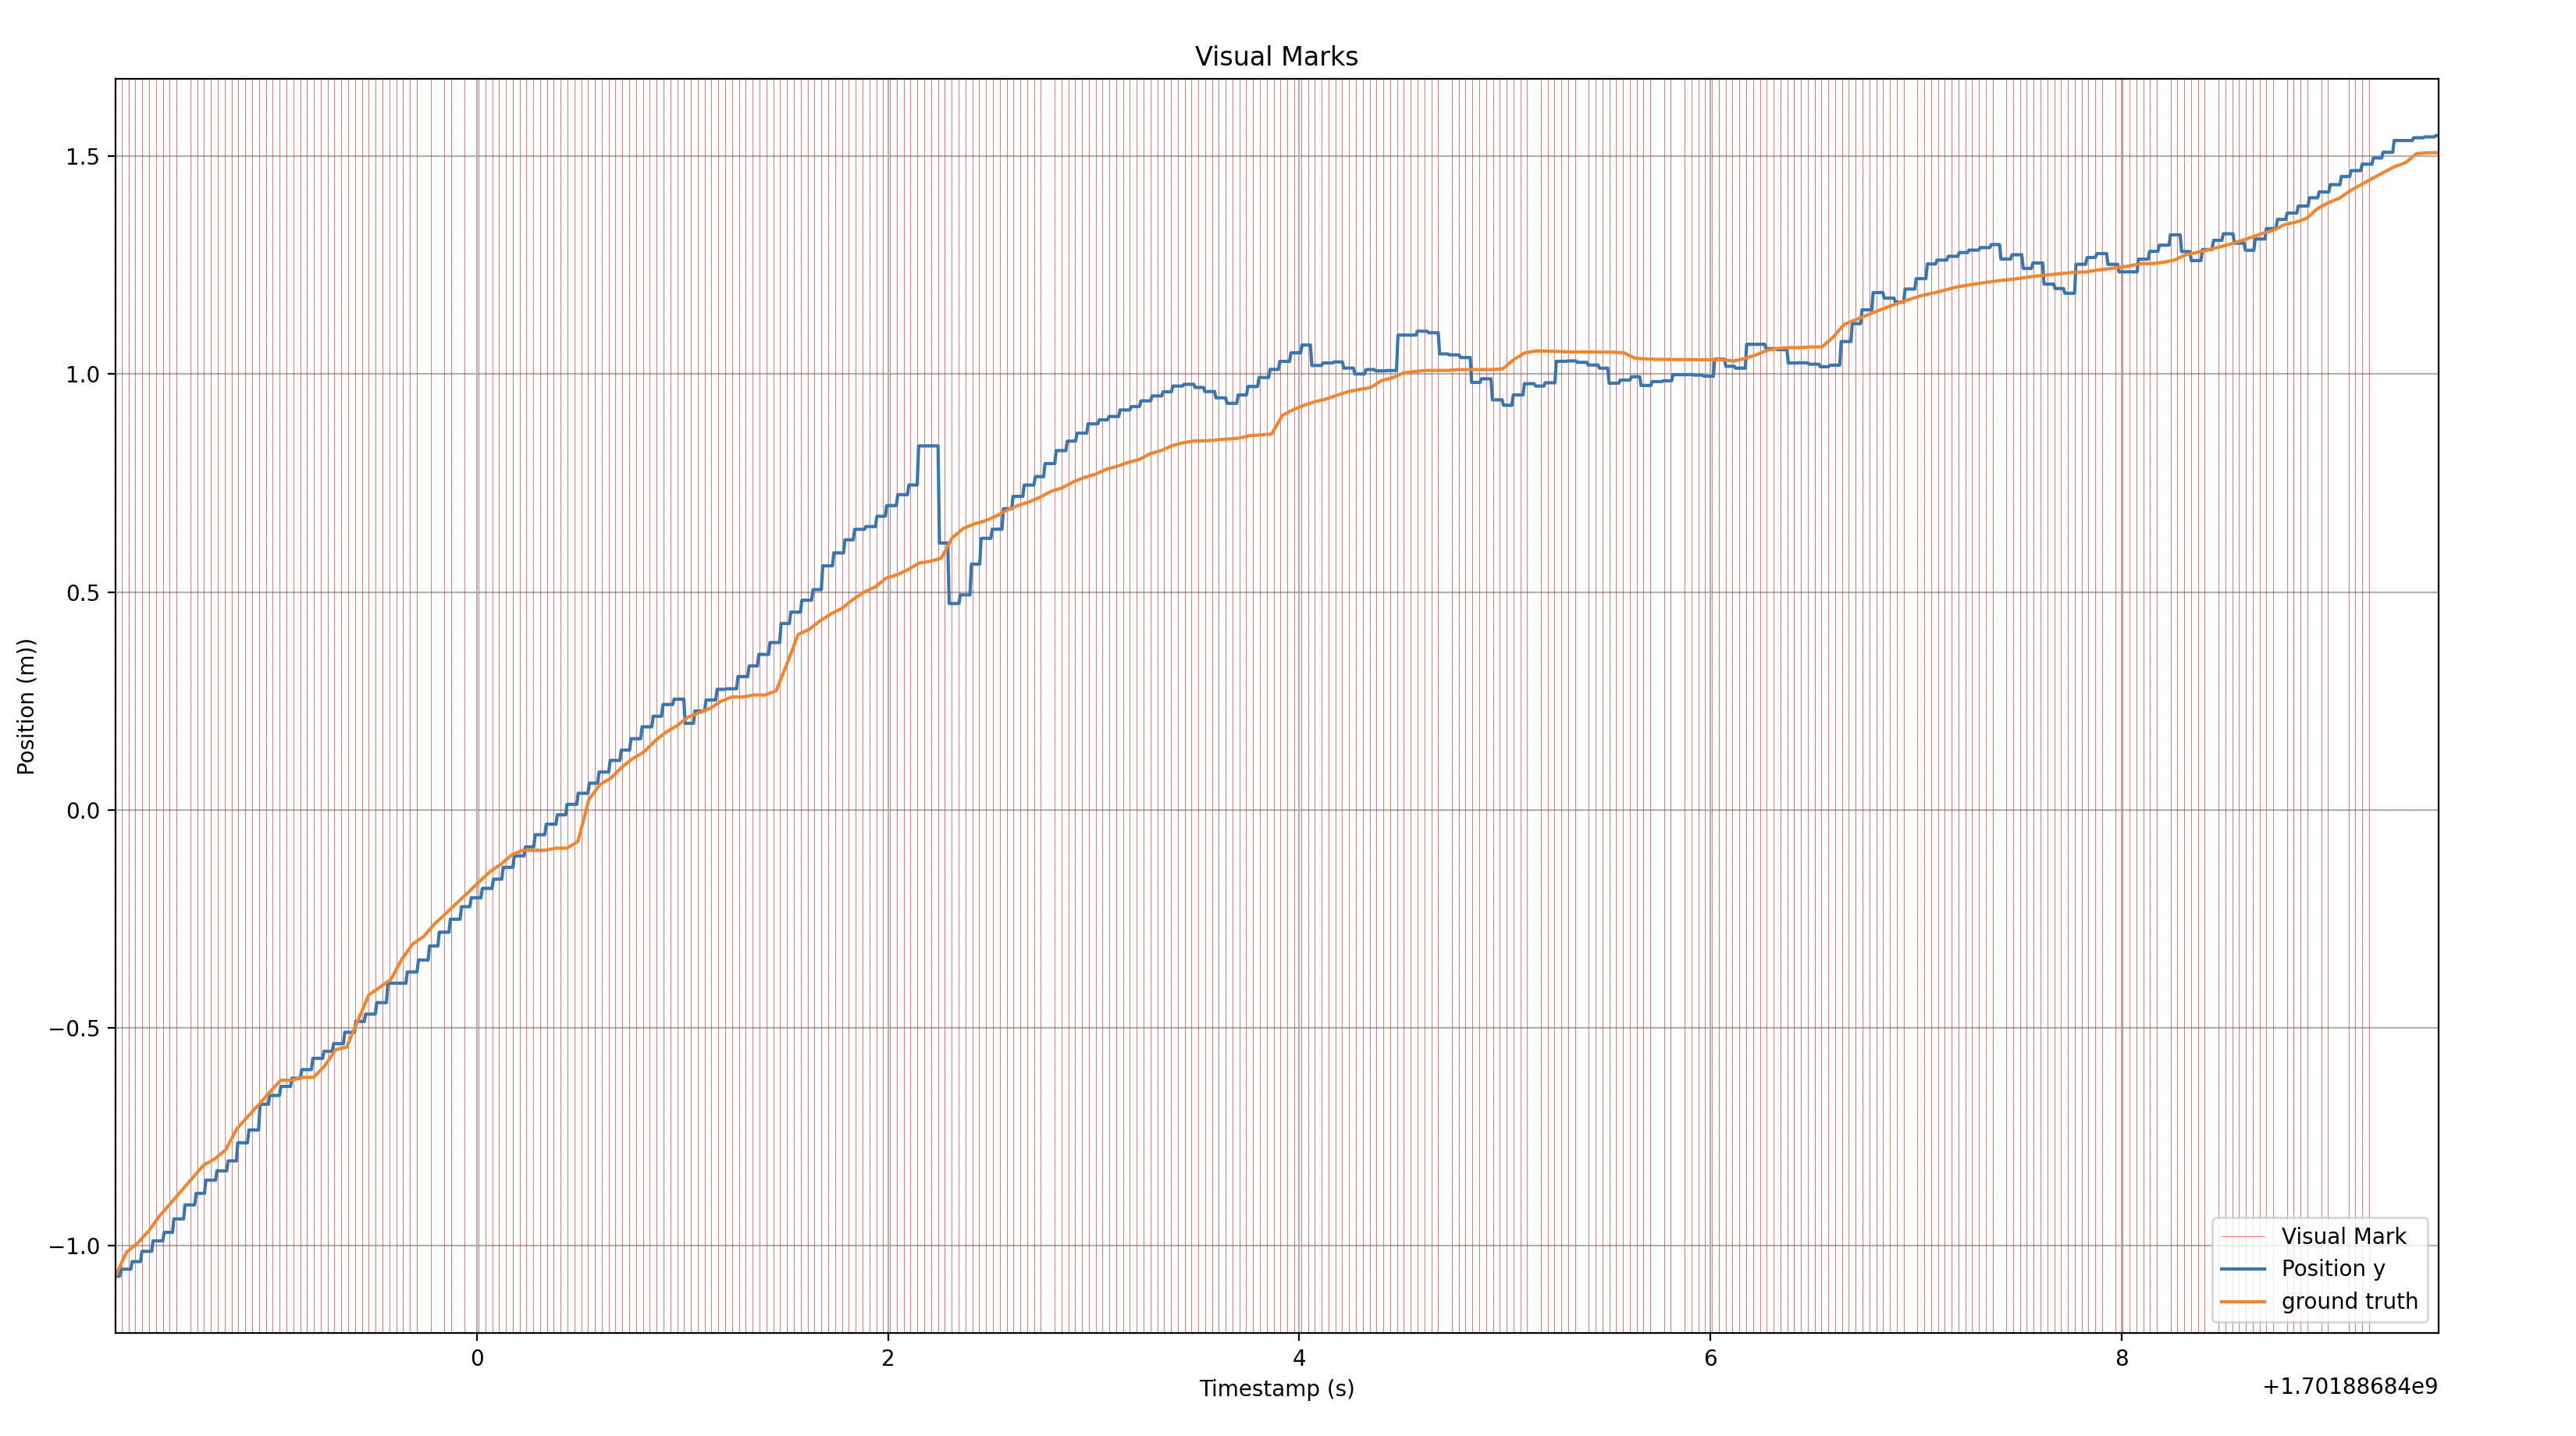
\includegraphics[width=.8\linewidth]{Pictures/sensor_fusion/Screenshot 2024-01-14 at 23.18.00.png}\hfill
    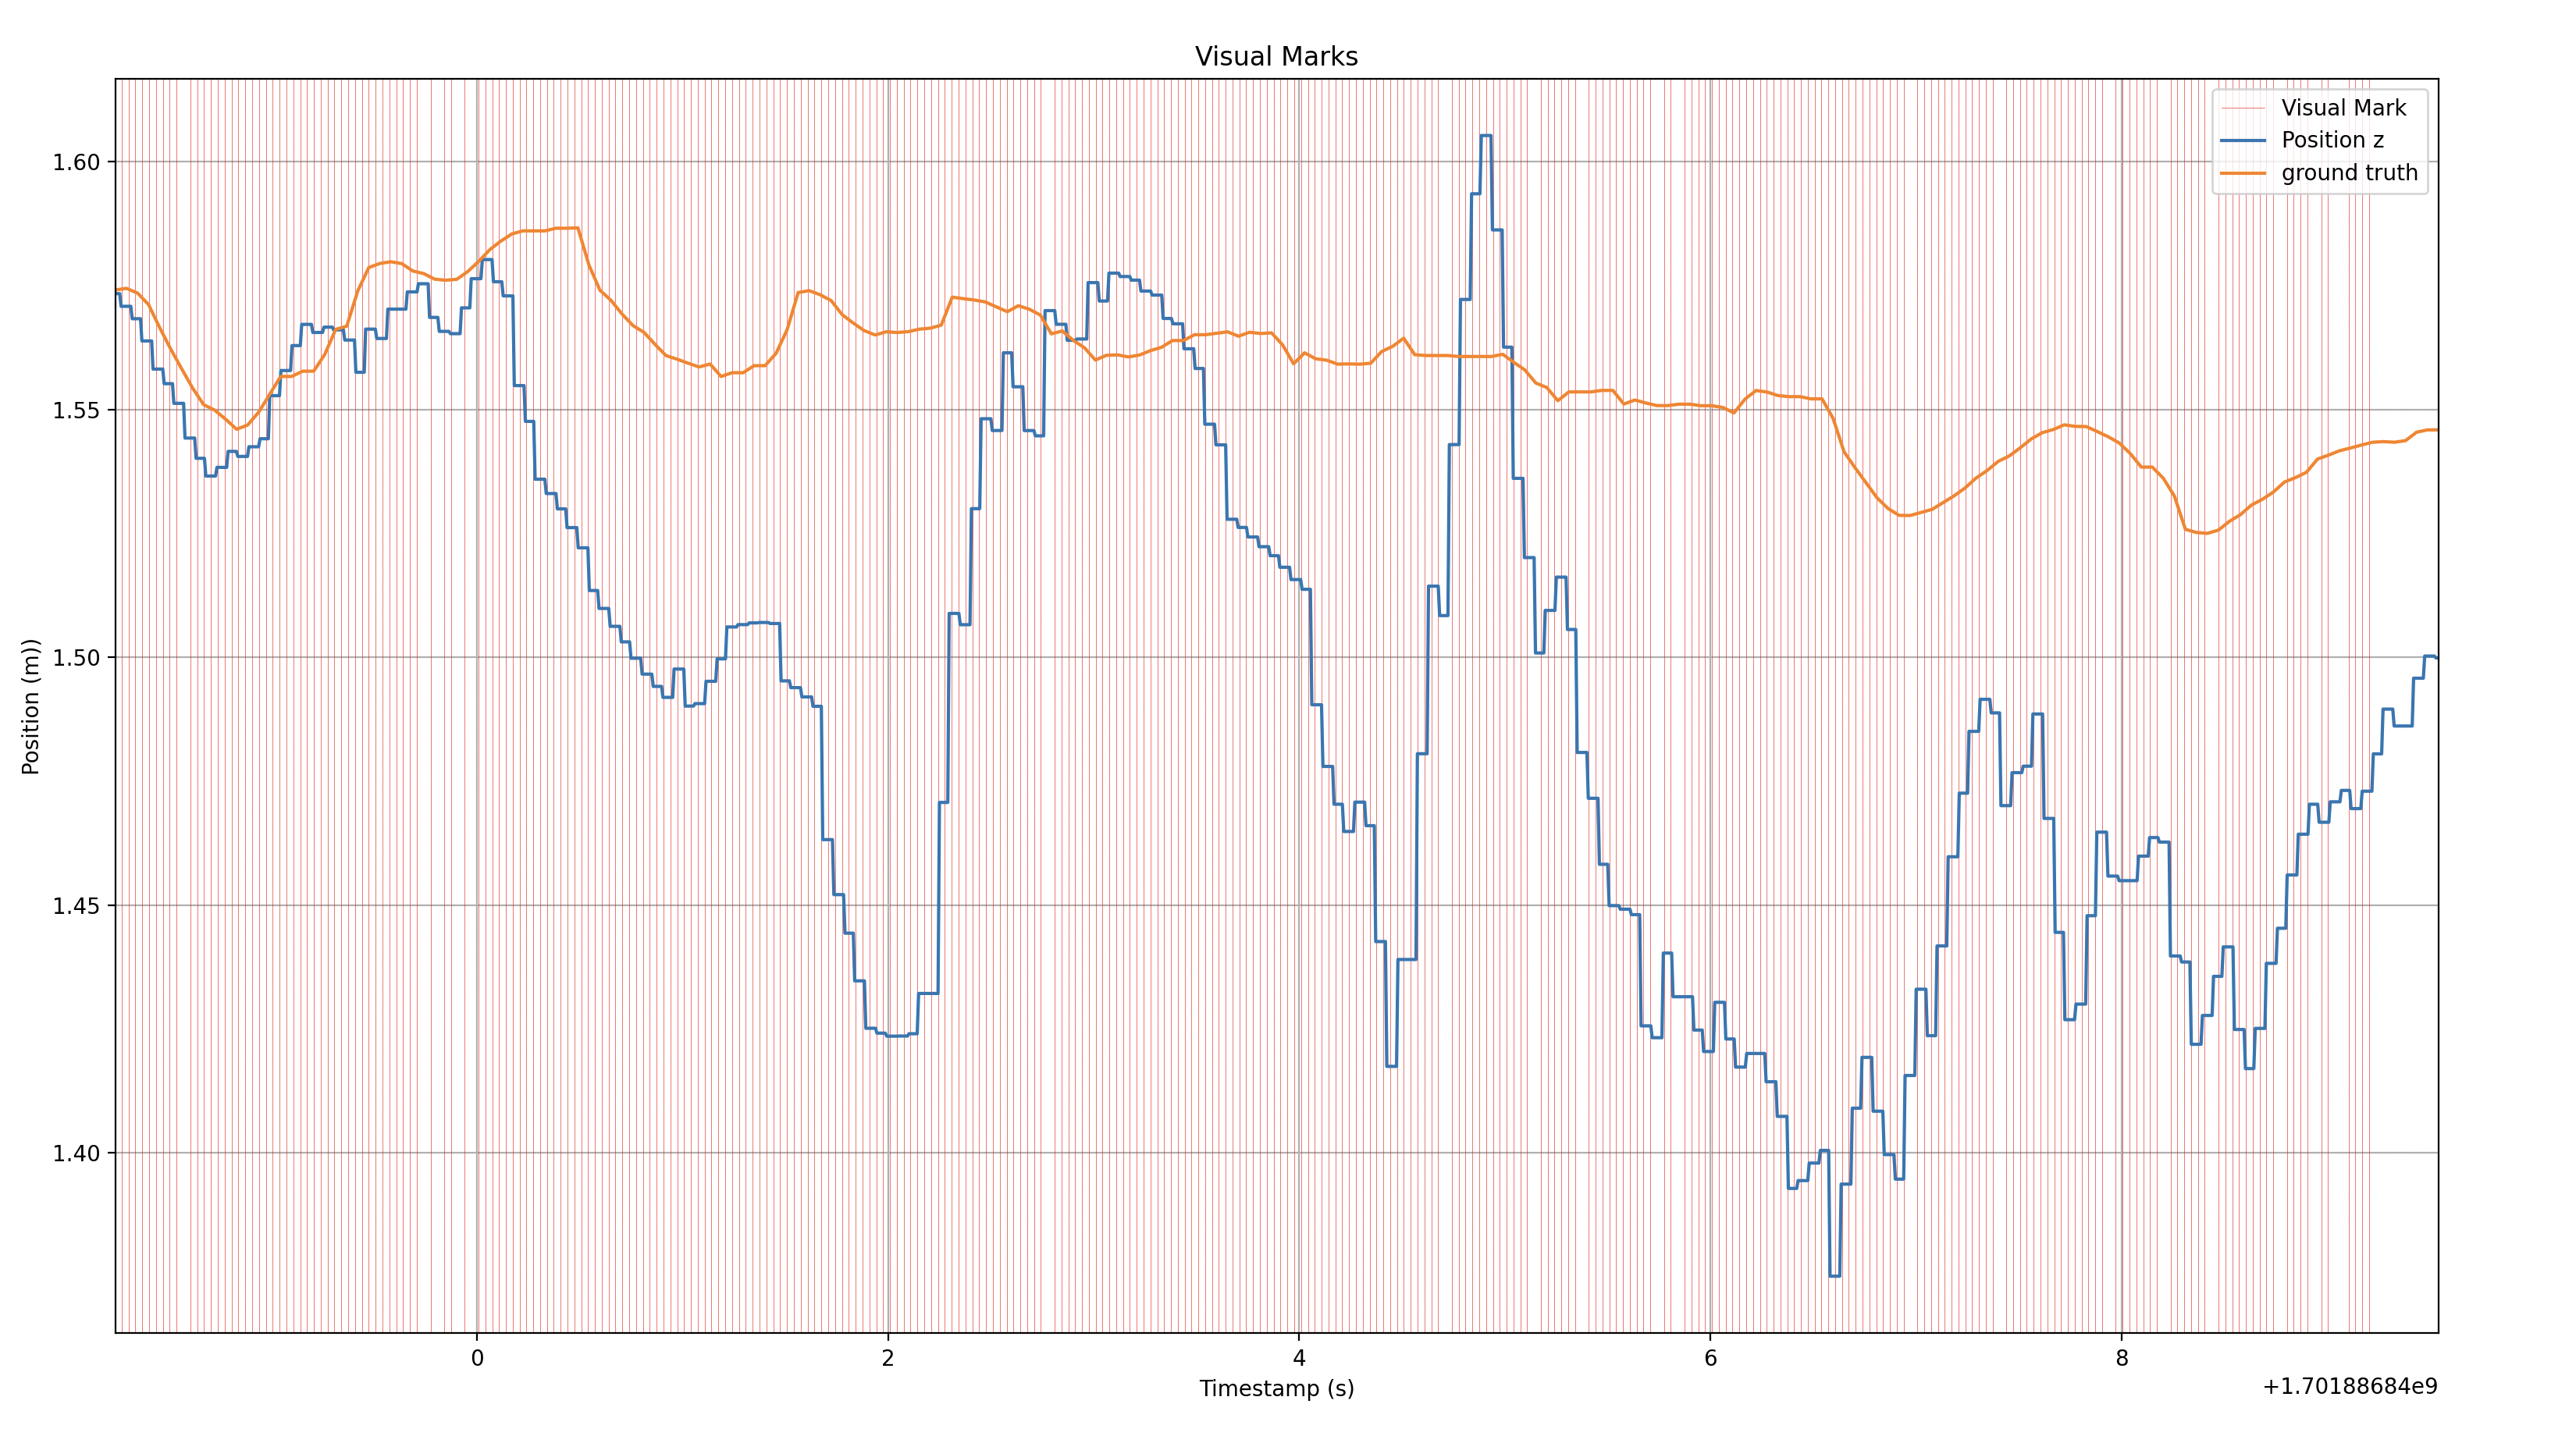
\includegraphics[width=.8\linewidth]{Pictures/sensor_fusion/Screenshot 2024-01-14 at 23.18.33.png}
    \caption{\textbf{Visual Marks of x, y or z Axis.} The red lines indicate update in EKF and its rate is 30Hz, while the IMU streaming for EKF prediction is 200Hz (IMU marks are not plotted.)}
    \label{fig:sensor_fusion_3_3}
\end{figure}


The Fig.\ref{fig:sensor_fusion_3_1} shows the trajectory of the drone in the x-y plane. There are two lines: the estimated trajectory (blue) and the ground truth (orange). The alignment between the estimated trajectory and the ground truth in the x-y plane exhibits the system's sophisticated capability to adapt and correct its path dynamically. The instances where the estimated trajectory deviates from the ground truth can be attributed to the challenging nature of segment-based localization, which relies heavily on the quality and consistency of visual data. Yet, the algorithm's ability to re-align with the ground truth path suggests a resilient matching strategy that can self-correct in response to new data inputs, a hallmark of intelligent systems.

\begin{figure}[H]
    \centering
    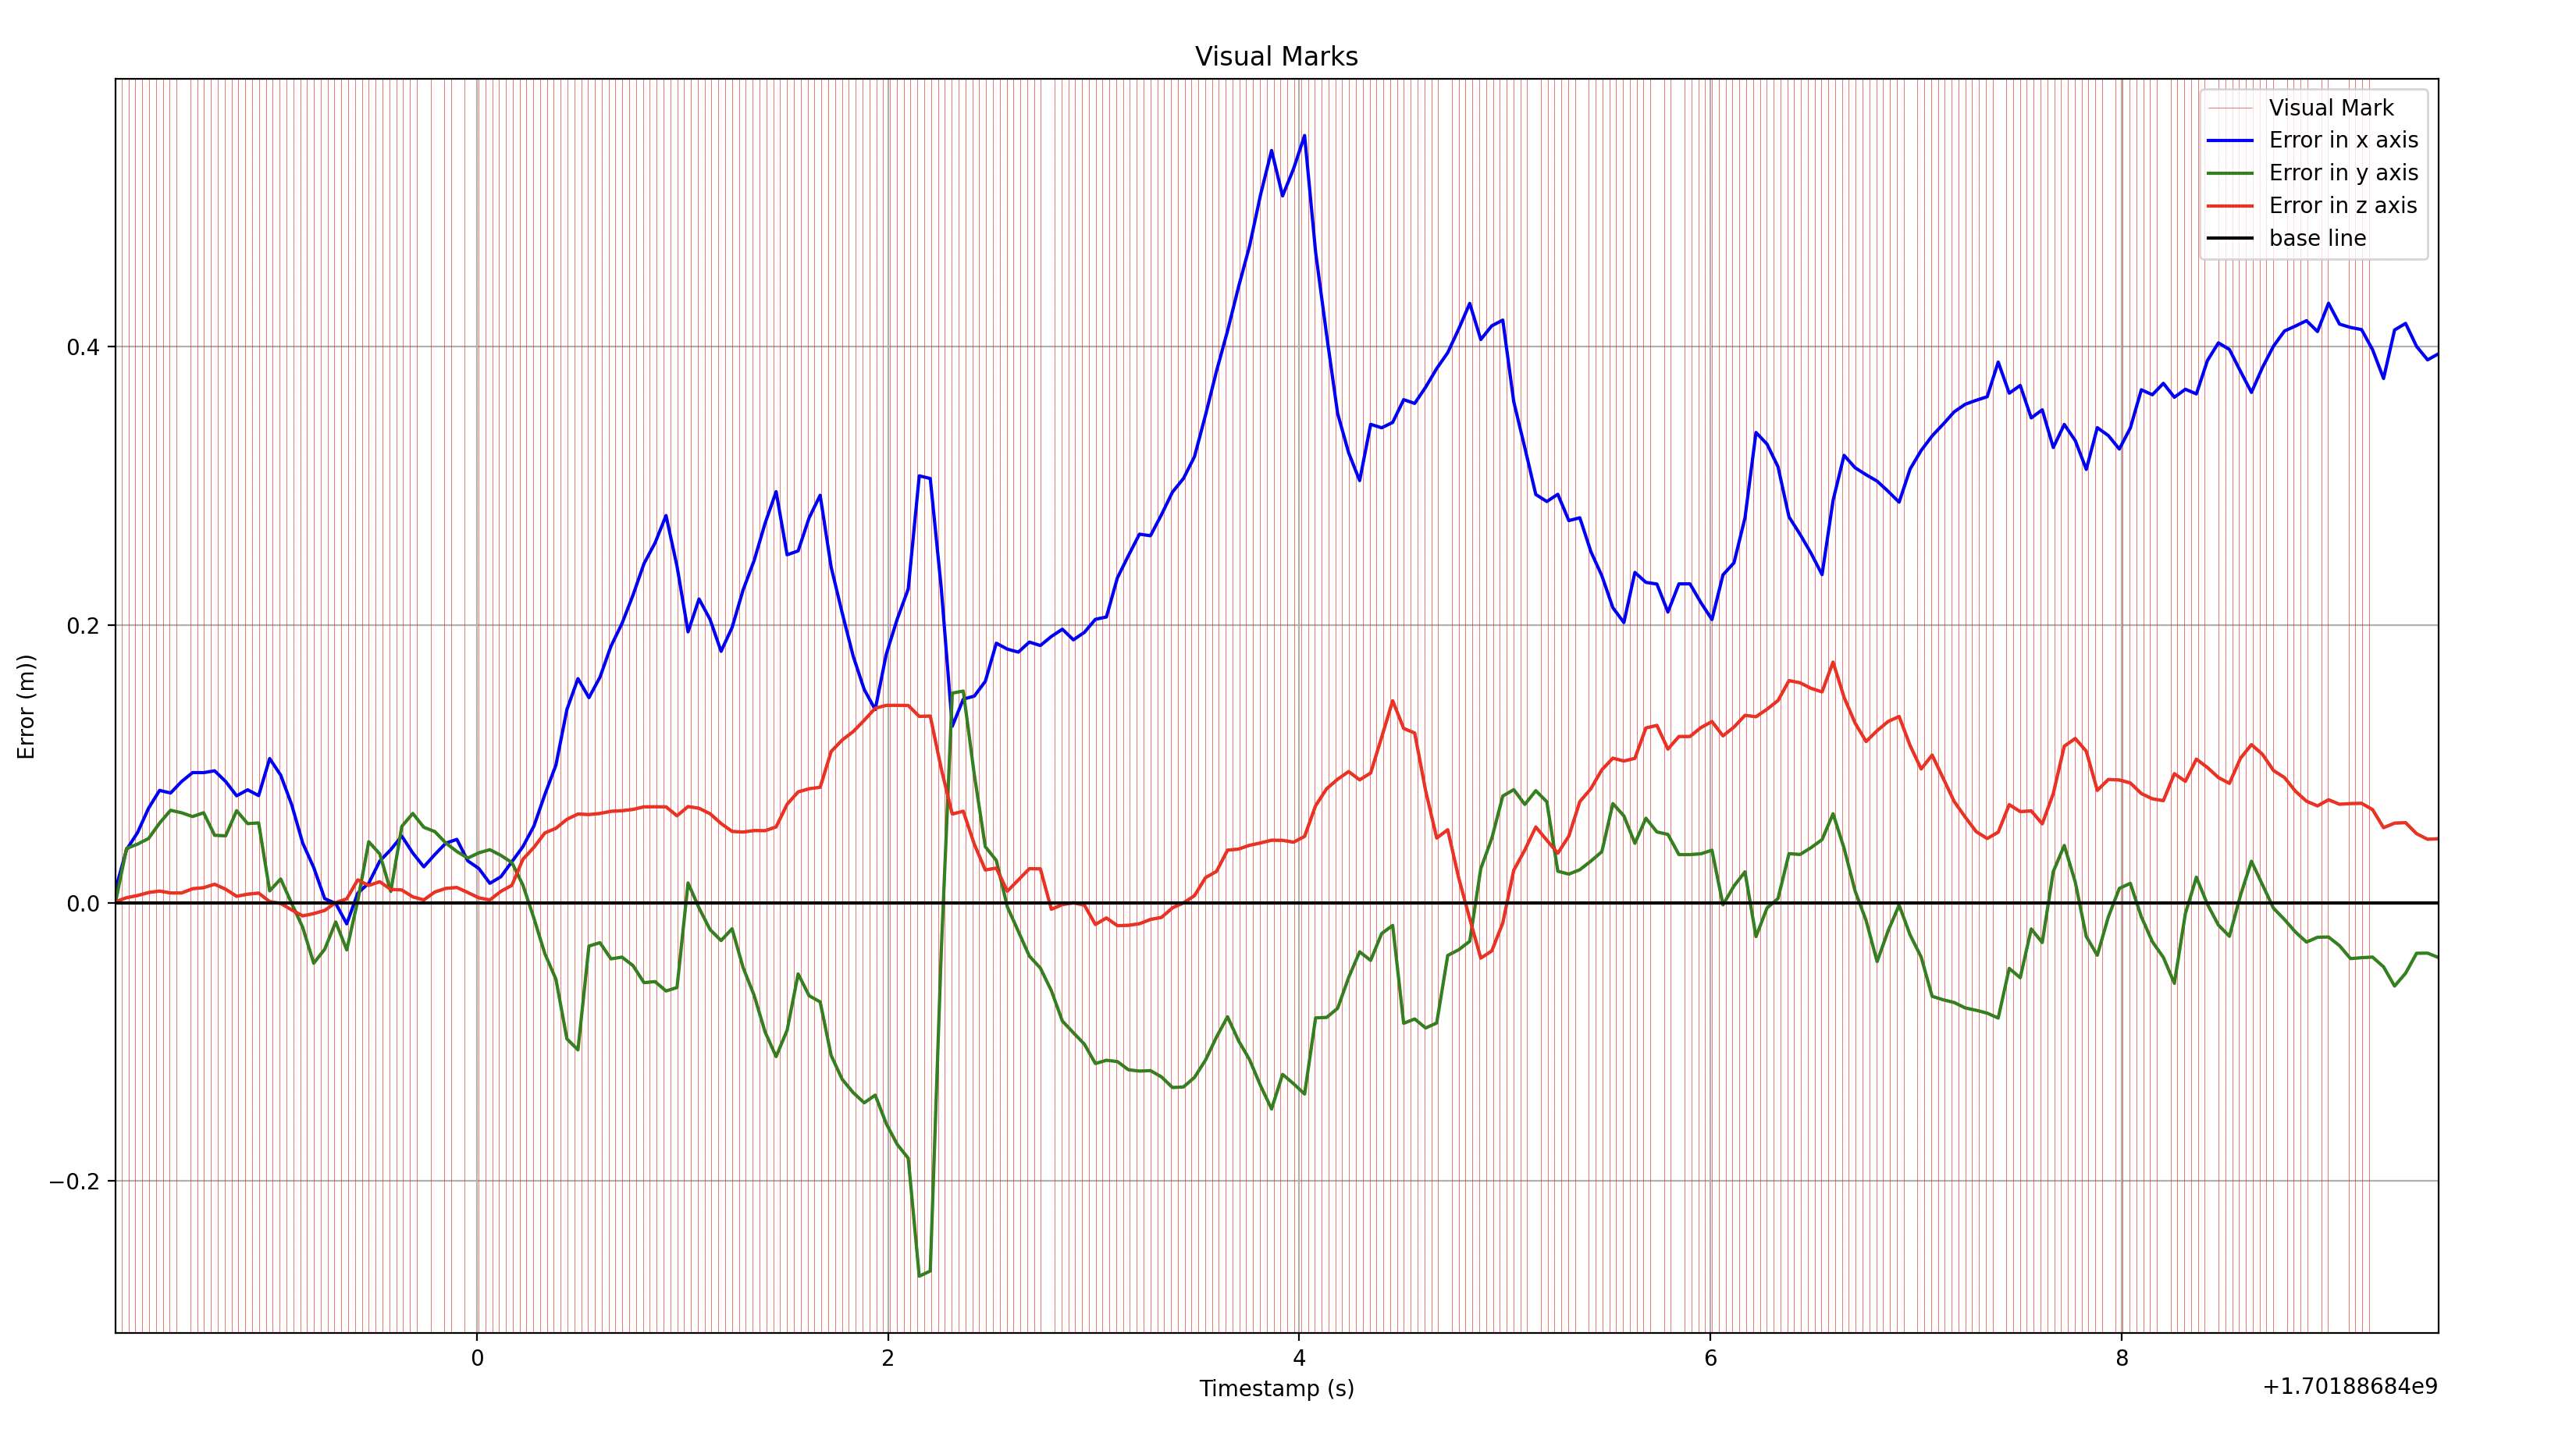
\includegraphics[width=.8\linewidth]{Pictures/sensor_fusion/Screenshot 2024-01-14 at 23.12.24.png}\hfill
    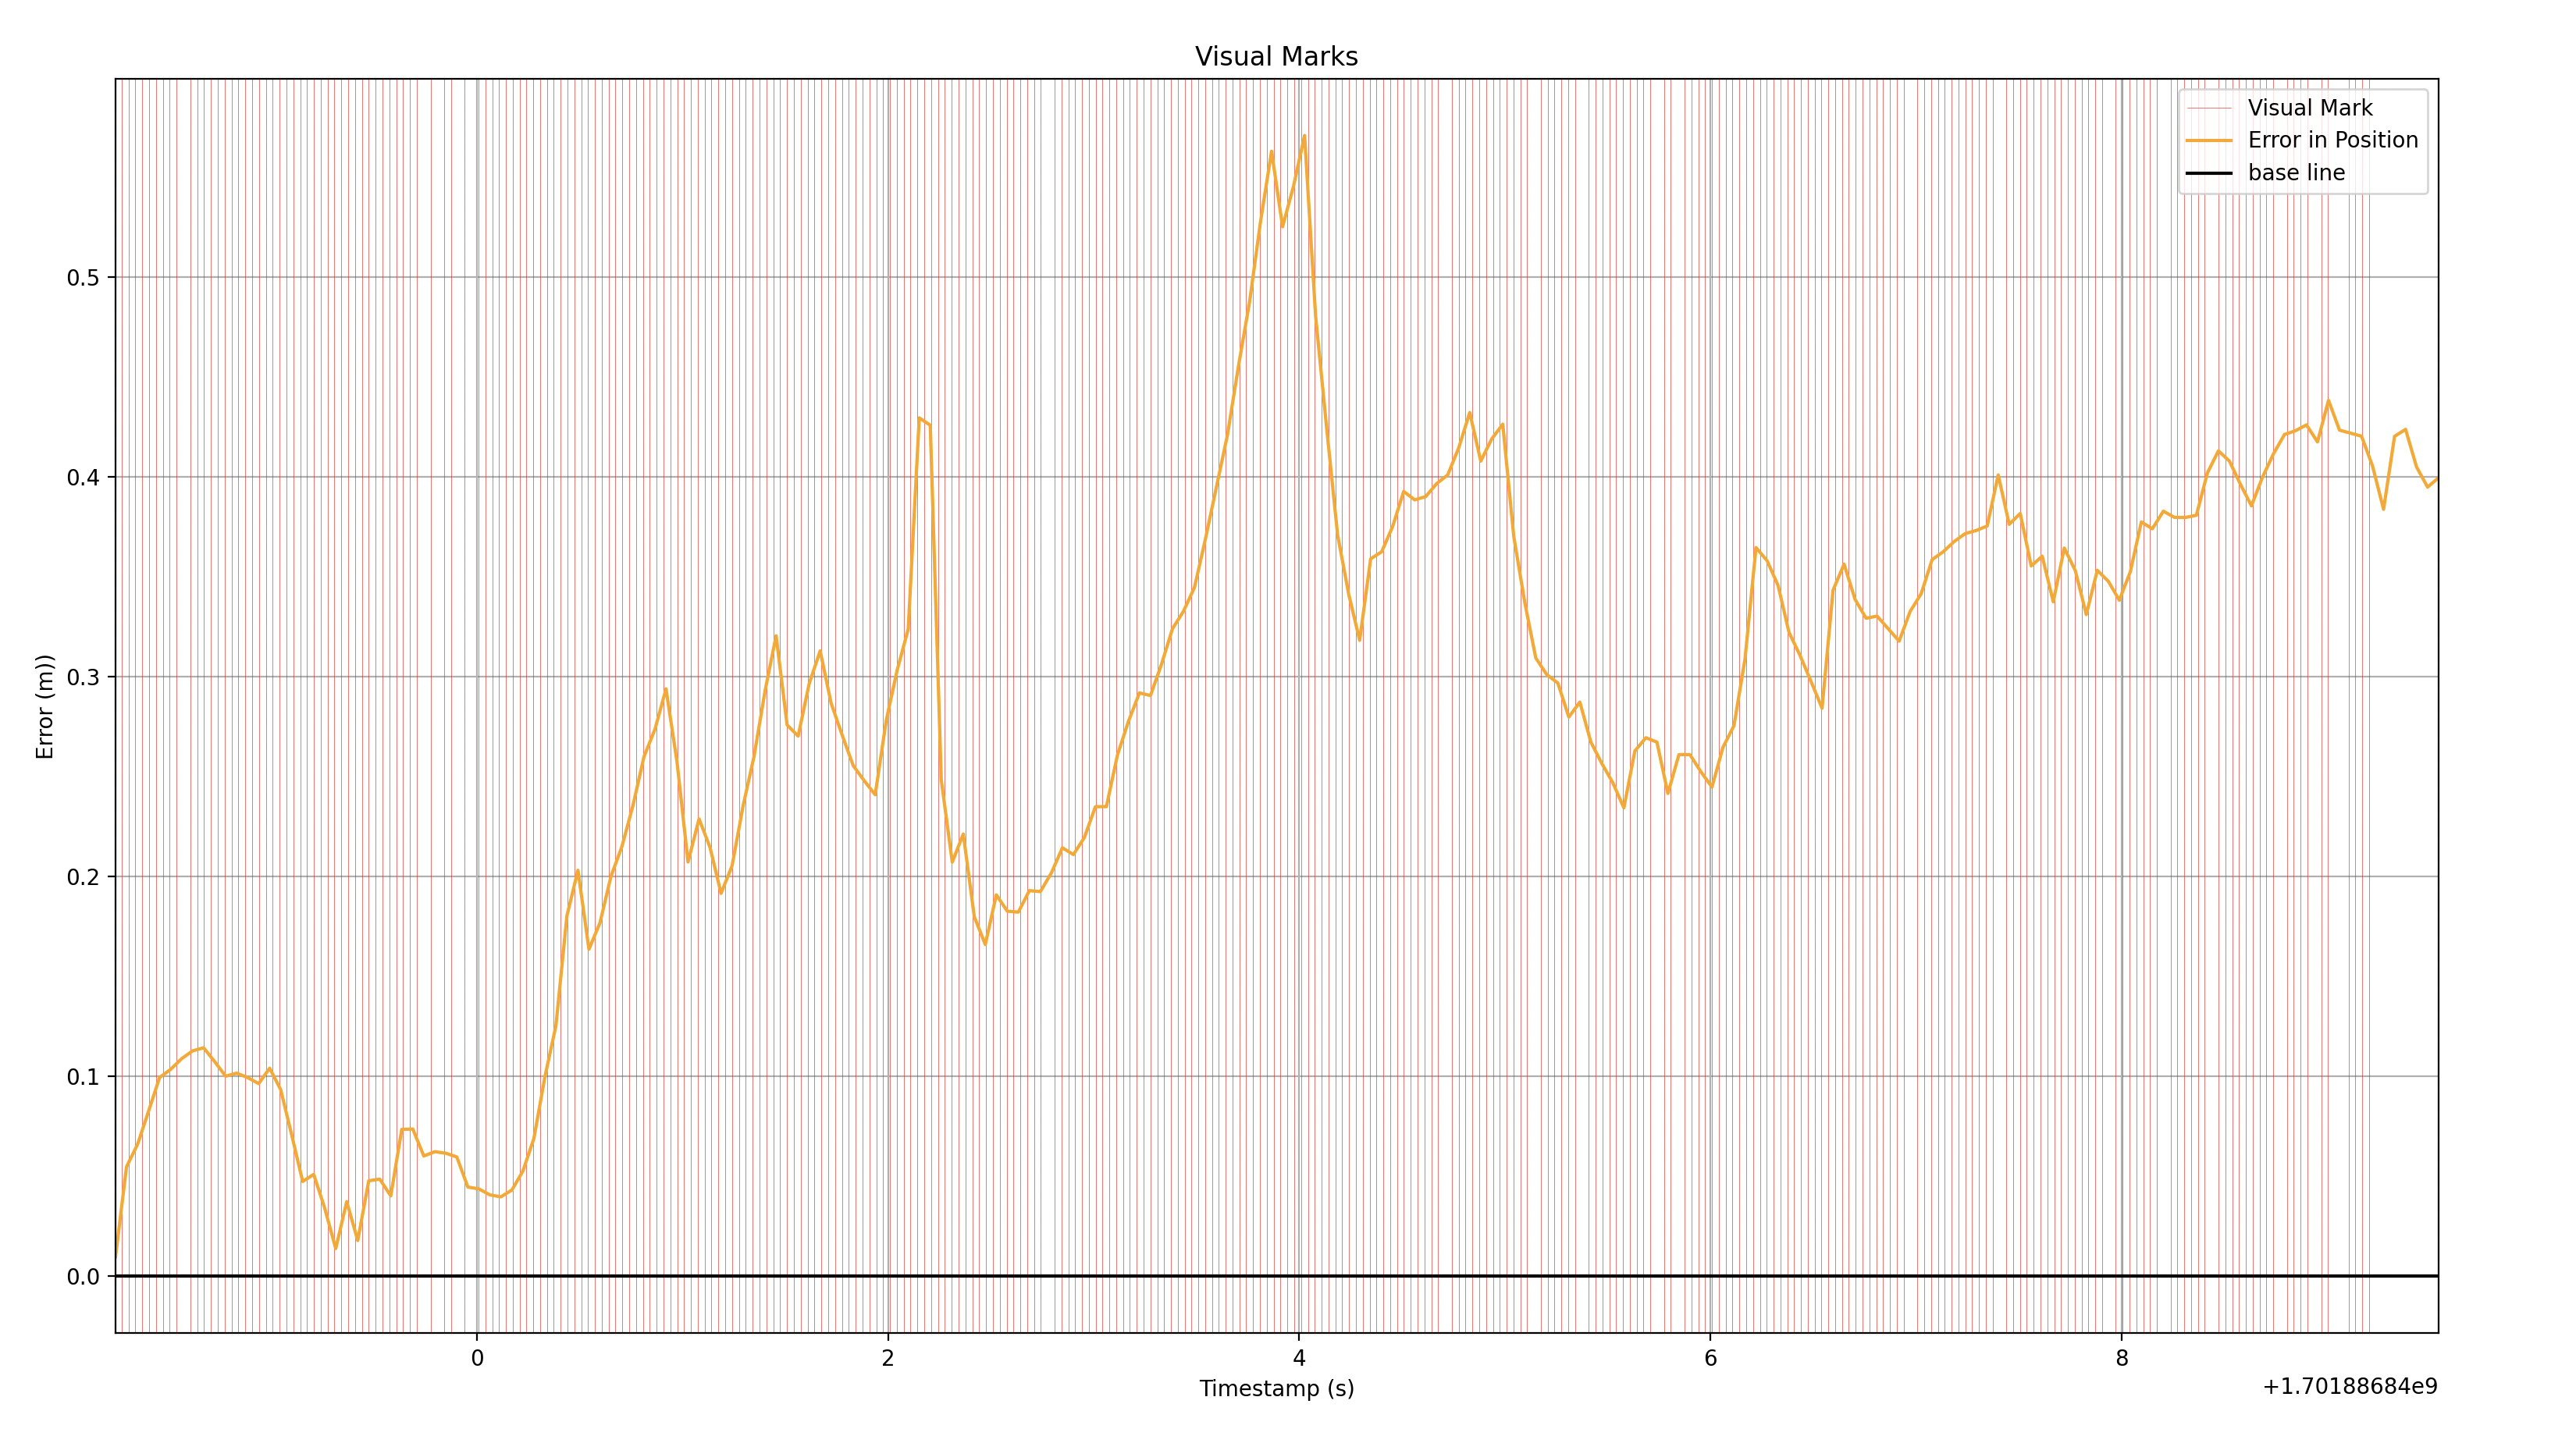
\includegraphics[width=.8\linewidth]{Pictures/sensor_fusion/Screenshot 2024-01-14 at 23.12.31.png}
    \caption{Error in x, y, z and Postion}
    \label{fig:sensor_fusion_3_4}
\end{figure}

In Fig.\ref{fig:sensor_fusion_3_3} and Fig. \ref{fig:sensor_fusion_3_4}, we examine the estimated and actual positions over time along the x, y, and z axes, including an analysis of their respective errors. The results display a commendable level of accuracy in the y and z-axis estimations, as indicated by the minimal fluctuation in these dimensions. This highlights the system's effectiveness in estimating positions along these axes.

However, a notable observation is made in the x-axis estimation. From the midpoint of the observed period to its end, there is a relative bias evident in the x-axis. This deviation can be attributed to the inherent characteristics of the 3D segments used in the pose estimation process. Specifically, the centroid of these segments, crucial for pose estimation, is influenced by the varying observation angles when segments are matched in the global map. 

This variance in observation angles can lead to discrepancies in the x-axis estimation, as the relative position of the centroid shifts depending on the drone's perspective. This effect underscores the complexity of segment-based localization and the challenges posed by the multi-dimensional nature of the task. Despite this, the overall consistency and accuracy in the y and z-axis estimations are promising, indicating that the system has a reliable performance in these aspects. The observed bias in the x-axis offers valuable insights into the limitations and areas for potential refinement in the algorithm, contributing to the ongoing development of more robust pose estimation methods.



Despite these small deviations, the overall consistency in the trajectory patterns suggests that the system is capable of stable performance under various conditions. This level of predictability is very important in real-time systems. Being able to foresee and correct errors is crucial for enhancing reliability during operations.
